\documentclass[a4paper, 11pt,reqno]{article}
\input{macro/package.tex}
\input{macro/environement}
% Header et footer

\pagestyle{fancy}
\fancyhead{}
\fancyfoot{}
\renewcommand{\headwidth}{\textwidth}
\renewcommand{\footrulewidth}{0.4pt}
\renewcommand{\headrulewidth}{0pt}
\renewcommand{\footruleskip}{5px}

\fancyfoot[R]{Olivier Glorieux}
%\fancyfoot[R]{Jules Glorieux}

\fancyfoot[C]{ Page \thepage }
\fancyfoot[L]{1BIOA - Lycée Chaptal}
%\fancyfoot[L]{MP*-Lycée Chaptal}
%\fancyfoot[L]{Famille Lapin}

\input{macro/newcommand.tex}
\geometry{hmargin=1.0cm, vmargin=2.5cm}


\newcommand{\type}{TD }
\excludecomment{correction}
%\newcommand{\type}{Correction TD }

\begin{document}

%--------------------------------------------------
%--------------------------------------------------
%-------------------------------------------------
%------------------------------------------------
\noindent\section{\large{Calculs de d\'eriv\'es}}
%-----------------------------------------------

\begin{exercice}  \; Avec des polyn\^omes.\\
	D\'eterminer le domaine de d\'efinition, le domaine de d\'erivabilit\'e et la d\'eriv\'ee des fonctions suivantes:
	\begin{enumerate}
		\begin{minipage}[t]{0.45\textwidth}
			\item $f(x)=\ddp\frac{x-1}{x+2}$
			\item $f(x)=\ddp\frac{1}{x^n}$, $n\in\N^{\star}$
			\item $f(x)=\ddp\frac{15x^4-30x^3+40x^2-20x+7}{(x-1)^5}$
		\end{minipage}
		\begin{minipage}[t]{0.45\textwidth}
			\item $f(x)=\left( \ddp\frac{3+x}{2x+1} \right)^4$
			\item $f(x)=(4-3x)^5$
			\item $f(x)=\ddp\frac{(4x-3)^3}{3x^2+1}$
		\end{minipage}
	\end{enumerate}
\end{exercice}
\begin{correction}  \; Avec des polyn\^omes.\\
	\begin{enumerate}
		\item $f(x)=\ddp\frac{x-1}{x+2}$\\
		      \noindent  La fonction $f$ est d\'efinie et d\'erivable sur $\R\setminus\lbrace -2\rbrace$. On obtient:
		      $\forall x\in\R\setminus\lbrace -2\rbrace,\quad f^{\prime}(x)=\ddp\frac{3}{(x+2)^2}$.
		\item $f(x)=\ddp\frac{1}{x^n}$, $n\in\N^{\star}$\\
		      \noindent  La fonction $f$ est d\'efinie et d\'erivable sur $\R^{\star}$ et on obtient:
		      $\forall x\in\R^{\star},\quad f^{\prime}(x)=\ddp\frac{-n}{x^{1+n}}.$
		\item $f(x)=\ddp\frac{15x^4-30x^3+40x^2-20x+7}{(x-1)^5}$ \\
		      \noindent  La fonction $f$ est d\'efinie et d\'erivable sur $\R\setminus\lbrace 1\rbrace$ et on obtient:
		      $\forall x\in\R\setminus\lbrace 1\rbrace,\quad f^{\prime}(x)=\ddp\frac{-15(x^4+2x^2+1)}{(x-1)^6}.$
		\item $f(x)=\left( \ddp\frac{3+x}{2x+1} \right)^4$\\
		      \noindent  La fonction $f$ est d\'efinie et d\'erivable sur $\R\setminus\lbrace -\ddp\demi\rbrace$ et on obtient:
		      $\forall x\not= -\ddp\demi,\quad f^{\prime}(x)=\ddp\frac{-20(3+x)^3}{(2x+1)^5}.$
		\item $f(x)=(4-3x)^5$
		      \begin{itemize}
			      \item[$\star$] Domaine de d\'efinition: La fonction $f$ est bien d\'efinie sur $\R$ et $\mathcal{D}_f=\R$.
			      \item[$\star$] Domaine de d\'erivabilit\'e: La fonction $f$ est d\'erivable sur $\R$ comme somme, compos\'ee et produit de fonctions d\'erivables.
			      \item[$\star$] Expression de la d\'eriv\'ee: pour tout $x\in\R$, $f^{\prime}(x)=-15(4-3x)^4$.
		      \end{itemize}
		\item $f(x)=\ddp\frac{(4x-3)^3}{3x^2+1}$
		      \begin{itemize}
			      \item[$\star$] Domaine de d\'efinition: La fonction $f$ est bien d\'efinie si $3x^2+1\not= 0$ ce qui est toujours vrai comme somme de deux termes positifs dont l'un est strictemlent positif. Ainsi $\mathcal{D}_f=\R$.
			      \item[$\star$] Domaine de d\'erivabilit\'e: La fonction $f$ est d\'erivable sur $\R$ comme somme, produit, compos\'ee et quotient de fonctions d\'erivables.
			      \item[$\star$] Expression de la d\'eriv\'ee: pour tout $x\in\mathcal{D}_{f^{\prime}}$, $f^{\prime}(x)=\ddp\frac{6(2x^2+3x+2)(4x-3)^2}{(3x^2+1)^2}$.
		      \end{itemize}
	\end{enumerate}
\end{correction}








\begin{exercice}   \; M\^emes questions, avec des racines et valeurs absolues.\\
	\begin{enumerate}
		\begin{minipage}[t]{0.45\textwidth}
			\item $f(x)=\sqrt{2x^2-3x+1}$
			\item $f(x)=x^n\sqrt{1-x}$, $n\in\N^{\star}$
			\item $f(x)=x\ddp\sqrt{\ddp\frac{1-x}{1+x}}$
		\end{minipage}
		\begin{minipage}[t]{0.45\textwidth}
			\item $f(x)=(\sqrt{x}+2x)^2$
			\item $f(x)=\sqrt{4x^2-1}$
			%\item $f(x)=\ddp\sqrt{\ddp\frac{x+1}{x-1}}$
			\item $f(x)=x|x|$
		\end{minipage}
	\end{enumerate}
\end{exercice}
\begin{correction}  \; Avec des racines et valeurs absolues.\\
	\begin{enumerate}
		\item $f(x)=\sqrt{2x^2-3x+1}$\\
		      \noindent La fonction $f$ est d\'efinie sur $\rbrack -\infty ,\ddp\demi\rbrack\cup\lbrack 1,+\infty\lbrack$ et d\'erivable sur $\rbrack -\infty ,\ddp\demi\lbrack\cup\rbrack 1,+\infty\lbrack$ et on obtient:
		      $\forall x\in\rbrack -\infty ,\ddp\demi\lbrack\cup\rbrack 1,+\infty\lbrack,\quad f^{\prime}(x)=\ddp\frac{4x-3}{2\sqrt{2x^2-3x+1}}.$
		\item $f(x)=x^n\sqrt{1-x}$, $n\in\N^{\star}$\\
		      \noindent  La fonction $f$ est d\'efinie sur $\rbrack -\infty,1\rbrack$ et d\'erivable sur $\rbrack -\infty,1\lbrack$ et on obtient:\\
		      \noindent $\forall x<1,\quad f^{\prime}(x)=\ddp\frac{x^{n-1}\left( x(-2n-1)+2n \right)}{2\sqrt{1-x}}.$
		\item $f(x)=x\ddp\sqrt{\ddp\frac{1-x}{1+x}}$\\
		      \noindent  La fonction $f$ est d\'efinie sur $\rbrack -1,1\rbrack$ et elle est d\'erivable sur $\rbrack -1,1\lbrack$ et on obtient:
		      $\forall x\in\rbrack -1,1\lbrack,\quad f^{\prime}(x)= \ddp\frac{-x^2-x+1}{\sqrt{1-x^2}(1+x)}.$
		\item $f(x)=(\sqrt{x}+2x)^2$\\
		      \noindent La fonction $f$ est d\'efinie sur $\R^{+}$ et elle est d\'erivable sur $\R^{+\star}$ et on obtient:\\
		      \noindent $\forall x>0,\quad f^{\prime}(x)=\ddp\frac{(2x+\sqrt{x})(1+4\sqrt{x})}{\sqrt{x}}.$
		\item $f(x)=\sqrt{4x^2-1}$
		      \begin{itemize}
			      \item[$\star$] Domaine de d\'efinition: La fonction $f$ est bien d\'efinie si $4x^2-1\geq 0$ et ainsi $\mathcal{D}_f=\left\rbrack -\infty,-\ddp\demi\right\rbrack\cup\left\lbrack \ddp\demi,+\infty\right\lbrack $.
			      \item[$\star$] Domaine de d\'erivabilit\'e: La fonction $f$ est d\'erivable sur $\left\rbrack -\infty,-\ddp\demi\right\lbrack\cup\left\rbrack \ddp\demi,+\infty\right\lbrack $ comme somme, produit et compos\'ee de fonctions d\'erivables car $f$ est d\'erivable si $4x^2-1>0$.
			      \item[$\star$] Expression de la d\'eriv\'ee: pour tout $x\in\mathcal{D}_{f^{\prime}}$, $f^{\prime}(x)=\ddp\frac{4x}{\sqrt{4x^2-1}}$.
		      \end{itemize}
		      %\item $f(x)=\ddp\sqrt{\ddp\frac{x+1}{x-1}}$
		\item  $f(x)=x|x|$\\
		      \begin{itemize}
			      \item[$\star$] Domaine de d\'efinition: La fonction $f$ est bien d\'efinie sur $\mathcal{D}_f=\R$.
			      \item[$\star$] Domaine de d\'erivabilit\'e: La fonction $f$ est d\'erivable sur $\R^{\star}$ comme compos\'ee et produit de fonctions d\'erivables car $x\not= 0$ afin que la valeur absolue soit d\'erivable.
			      \item[$\star$] Expression de la d\'eriv\'ee: pour tout $x\in\mathcal{D}_{f^{\prime}}$, $f^{\prime}(x)=\left\lbrace\begin{array}{ll}
					            -2x & \hbox{si}\ x<0\vsec \\
					            2x  & \hbox{si}\ x>0
				            \end{array}\right.$ car $f(x)=\left\lbrace\begin{array}{ll}
					            -x^2 & \hbox{si}\ x>0 \vsec \\
					            x^2  & \hbox{si}\ x<0
				            \end{array}\right.$.
		      \end{itemize}
	\end{enumerate}
\end{correction}







\begin{exercice}   \; M\^emes questions, avec des exponentielles et logarithmes.\\
	\begin{enumerate}
		\begin{minipage}[t]{0.45\textwidth}
			\item $f(x)=x^x$
			\item $f(x)=e^{-\frac{x^2}{2}}$
			\item $f(x)=\ln{|x|}$
			\item $f(x)=\ln{|(x^2+1)^3|}$
		\end{minipage}
		\begin{minipage}[t]{0.45\textwidth}
			\item $f(x)=\ln{\left(\ddp\frac{x^x-1}{x^x+1}  \right)}$
			\item $f(x)=\ddp\frac{1}{\ln{(x)}}$
			\item $f(x)=\ln{(\ln{x})}$
			\item $f(x)=|\ln{(x)}|$
		\end{minipage}
	\end{enumerate}
\end{exercice}
\begin{correction}  \; Avec des exponentielles et logarithmes.\\
	\begin{enumerate}
		\item $f(x)=x^x=e^{x\ln{x}}$\\
		      \noindent  La fonction $f$ est d\'efinie et d\'erivable sur $\R^{+\star}$ et on obtient:
		      $\forall x>0,\quad f^{\prime}(x)=x^x\left( \ln{x}+1\right).$
		\item
		      $f(x)=e^{-\frac{x^2}{2}}$\\
		      \noindent  La fonction $f$ est d\'efinie et d\'erivable sur $\R$ et on obtient:
		      $\forall x\in\R,\quad f^{\prime}(x)=-xe^{\frac{-x^2}{2}}$.
		\item $f(x)=\ln{|x|}$\\
		      \noindent  La fonction $f$ est d\'efinie et d\'erivble sur $\R^{\star}$. Comme il y a une valeur absolue, on \'etudie des cas:
		      \begin{itemize}
			      \item[$\star$] Si $x> 0$, alors $f(x)=\ln{(x)}$ et $f^{\prime}(x)=\ddp\frac{1}{x}$.
			      \item[$\star$]  Si $x< 0$, alors $f(x)=\ln{(-x)}$ et $f^{\prime}(x)=\ddp\frac{-1}{-x}=\ddp\frac{1}{x}$.
		      \end{itemize}
		      Ainsi, dans tous les cas, sur $\R^{\star}$, on obtient que: $f^{\prime}(x)=\ddp\frac{1}{x}$.
		\item
		      $f(x)=\ln{|(x^2+1)^3|}$\\
		      \noindent Comme $1+x^2>0$, la fonction $f$ est d\'efinie et d\'erivable sur $\R$ et la valeur absolue est inutile. Ainsi, on a: $\forall x\in\R,\quad f(x)=\ln{(x^2+1)^3}$ et $f^{\prime}(x)=\ddp\frac{6x}{1+x^2}$.
		\item $f(x)=\ln{\left(\ddp\frac{x^x-1}{x^x+1}  \right)}$\\
		      \noindent La fonction $f$ est d\'efinie et d\'erivable sur $\rbrack 1,+\infty\lbrack$ et on obtient:
		      $\forall x>1,\quad f^{\prime}(x)=\ddp\frac{2x^x(1+\ln{x})}{(x^x-1)(x^x+1)}.$
		\item $f(x)=\ddp\frac{1}{\ln{(x)}}$\\
		      \begin{itemize}
			      \item[$\star$] Domaine de d\'efinition: La fonction $f$ est bien d\'efinie si $x>0$ et $\ln{x}\not= 0\Leftrightarrow x\not= 1$. Ainsi $\mathcal{D}_f=\rbrack 0,1\lbrack\cup\rbrack 1,+\infty\lbrack$.
			      \item[$\star$] Domaine de d\'erivabilit\'e: La fonction $f$ est d\'erivable sur $\mathcal{D}_f$ comme quotient de fonctions d\'erivables.
			      \item[$\star$] Expression de la d\'eriv\'ee: pour tout $x\in\mathcal{D}_{f^{\prime}}$, $f^{\prime}(x)=\ddp\frac{-1}{x(\ln{(x)})^2}$.
		      \end{itemize}
		\item $f(x)=\ln{(\ln{x})}$\\
		      \begin{itemize}
			      \item[$\star$] Domaine de d\'efinition: La fonction $f$ est bien d\'efinie si $x>0$ et $\ln{(x)}>0$. Ainsi $\mathcal{D}_f=\rbrack 1,+\infty\lbrack$.
			      \item[$\star$] Domaine de d\'erivabilit\'e: La fonction $f$ est d\'erivable sur $\rbrack 1,+\infty\lbrack$ comme compos\'ee de fonctions d\'erivables.
			      \item[$\star$] Expression de la d\'eriv\'ee: pour tout $x\in\mathcal{D}_{f^{\prime}}$, $f^{\prime}(x)=\ddp\frac{1}{x\ln{(x)}}$.
		      \end{itemize}
		\item $f(x)=|\ln{(x)}|$\\
		      \begin{itemize}
			      \item[$\star$] Domaine de d\'efinition: La fonction $f$ est bien d\'efinie si $x>0$ et $\mathcal{D}_f=\R^{+\star}$.
			      \item[$\star$] Domaine de d\'erivabilit\'e: La fonction $f$ est d\'erivable sur $\R^{+\star}\setminus\lbrace 1\rbrace$ comme compos\'ee de fonctions d\'erivables et car $\ln{x}\not= 0$ pour que la valeur absolue soit bien d\'erivable.
			      \item[$\star$] Expression de la d\'eriv\'ee: pour tout $x\in\mathcal{D}_{f^{\prime}}$, $f^{\prime}(x)=\left\lbrace\begin{array}{ll}
					            -\ddp\frac{1}{x} & \hbox{si}\ x\in\rbrack 0,1\lbrack\vsec  \\
					            \ddp\frac{1}{x}  & \hbox{si}\ x\in\rbrack 1,+\infty\lbrack
				            \end{array}\right.$ car $f(x)=\left\lbrace\begin{array}{ll}
					            -\ln{(x)} & \hbox{si}\ x\in\rbrack 0,1\rbrack\vsec  \\
					            \ln{(x)}  & \hbox{si}\ x\in\rbrack 1,+\infty\lbrack
				            \end{array}\right.$.
		      \end{itemize}

	\end{enumerate}
\end{correction}




\begin{exercice}  \;  M\^emes questions, avec des fonctions trigonom\'etriques.\\
	\begin{enumerate}
		\begin{minipage}[t]{0.45\textwidth}
			\item $f(x)=\tan{\left( \ddp\frac{2x}{1+x^2} \right)}$
			\item $f(x)=\cos^4{x}$
		\end{minipage}
		\begin{minipage}[t]{0.45\textwidth}
			\item $f(x)=(\sin{(x)})e^{\cos{x}}$
			\item $f(x)=\sin{(\sin{(\sin{x})})}$
			\item $f(x)=\cos{(\sqrt{x})}$
		\end{minipage}
	\end{enumerate}
\end{exercice}
\begin{correction}  \; Avec des fonctions trigonom\'etriques.\\
	\begin{enumerate}
		\item $f(x)=\tan{\left( \ddp\frac{2x}{1+x^2} \right)}$\\
		      La fonction $f$ est d\'efinie et d\'erivable si $x$ v\'erifie: $\forall k\in\Z,\quad \ddp\frac{2x}{1+x^2}\not= \ddp\frac{\pi}{2}+k\pi$. On obtient alors sur cet ensemble: $f^{\prime}(x)=\ddp\frac{2(1-x^2)}{(1+x^2)^2}\left( 1+\tan^2{\left( \ddp\frac{2x}{1+x^2} \right)} \right)$.
		\item $f(x)=\cos^4{x}$\\
		      La fonction $f$ est d\'efinie et d\'erivable sur $\R$ et on obtient: $\forall x\in\R,\quad f^{\prime}(x)=-4\sin{(x)}\cos^3{(x)}.$
		\item $f(x)=(\sin{(x)})e^{\cos{x}}$\\
		      \begin{itemize}
			      \item[$\star$] Domaine de d\'efinition: La fonction $f$ est bien d\'efinie sur $\R$ et $\mathcal{D}_f=\R$.
			      \item[$\star$] Domaine de d\'erivabilit\'e: La fonction $f$ est d\'erivable sur $\R$ comme compos\'ee et produit de fonctions d\'erivables.
			      \item[$\star$] Expression de la d\'eriv\'ee: pour tout $x\in\mathcal{D}_{f^{\prime}}$, $f^{\prime}(x)=\left( \cos{(x)}-\sin^2{(x)}  \right)e^{\cos{x}}$.
		      \end{itemize}
		\item $f(x)=\sin{(\sin{(\sin{x})})}$\\
		      \begin{itemize}
			      \item[$\star$] Domaine de d\'efinition: La fonction $f$ est bien d\'efinie sur $\R$ et $\mathcal{D}_f=\R$.
			      \item[$\star$] Domaine de d\'erivabilit\'e: La fonction $f$ est d\'erivable sur $\R$ comme compos\'ee de fonctions d\'erivables.
			      \item[$\star$] Expression de la d\'eriv\'ee: pour tout $x\in\mathcal{D}_{f^{\prime}}$, $f^{\prime}(x)=\cos{(x)}\times \cos{(\sin{(x)})}\times \cos{(\sin{(\sin{x})})}$.
		      \end{itemize}
		\item $f(x)=\cos{(\sqrt{x})}$\\
		      \begin{itemize}
			      \item[$\star$] Domaine de d\'efinition: La fonction $f$ est bien d\'efinie si $x\geq 0$ et $\mathcal{D}_f=\R^+$.
			      \item[$\star$] Domaine de d\'erivabilit\'e: La fonction $f$ est d\'erivable sur $\R^{+\star}$ comme compos\'ee de fonctions d\'erivables car $x>0$ afin que la racine carr\'ee soit bien d\'erivable.
			      \item[$\star$] Expression de la d\'eriv\'ee: pour tout $x\in\mathcal{D}_{f^{\prime}}$, $f^{\prime}(x)=\ddp\frac{-\sin{(\sqrt{x})}}{2\sqrt{x}}$.
		      \end{itemize}
	\end{enumerate}
\end{correction}



%-----------------------------------------------
\begin{exercice}   \;
	Calculer la d\'eriv\'ee de $f:\ x\mapsto a^{\frac{1}{\sqrt{a^2-x^2}}}$ avec $a\in\R^{+\star}\setminus\lbrace 1\rbrace$.
\end{exercice}
\begin{correction}  \;
	La fonction $f$ est d\'efinie et d\'erivable sur $\rbrack -a,a\lbrack$. Le calcul de sa d\'eriv\'ee donne:
	$$f^{\prime}(x)=a^{\frac{1}{\sqrt{a^2-x^2}}}\times\ddp\frac{x\ln{a}}{(a^2-x^2)\sqrt{a^2-x^2}}.$$
\end{correction}

\begin{correction}   \;
	\textbf{Soit $x_0\in \R$ fix\'e, et soit $f$ une fonction d\'efinie au voisinage de $x_0$ et d\'erivable en $x_0$.}\vsec\\
	On reconna\^it un taux d'accroissement : $\ddp\lim\limits_{h \to 0} \frac{f(x_0+h) - f(x_0)}{h} = \lim\limits_{h \to 0} \frac{f(x_0+h) - f(x_0)}{(x_0+h)-x_0} =$ \fbox{$f'(x_0)$} car $f$ est d\'erivable en $x_0$. (On peut d\'etailler en posant par exemple le changement de variable $X=x-x_0$).\\
	On fait appara\^itre deux taux d'accroissement :
	$$\ddp \frac{f(x_0+h) - f(x_0-h)}{h} = \frac{f(x_0+h) -f(x_0)+f(x_0)-f(x_0-h)}{h} =  \frac{f(x_0+h) -f(x_0)}{(x_0+h)-x_0}+ \frac{f(x_0)-f(x_0-h)}{x_0-(x_0-h)}.$$
	Or $f$ est d\'erivable en $x_0$ donc $\ddp\lim\limits_{h \to 0} \frac{f(x_0+h) -f(x_0)}{(x_0+h)-x_0} = f'(x_0)$ et $\ddp\lim\limits_{h \to 0} \frac{f(x_0)-f(x_0-h)}{x_0-(x_0-h)} = f'(x_0)$.\\
	On en d\'eduit que \fbox{$\ddp\lim\limits_{h \to 0}  \frac{f(x_0+h) - f(x_0-h)}{h} = 2f'(x_0)$}.
\end{correction}




%-----------------------------------------------
\begin{exercice}   \;
	Soit $x_0\in \R$ fix\'e, et soit $f$ une fonction d\'efinie au voisinage de $x_0$ et d\'erivable en $x_0$.\vsec\\
	Calculer \, $\ddp\lim\limits_{h \to 0} \frac{f(x_0+h) - f(x_0)}{h}$ \, et \,  $\ddp\lim\limits_{h \to 0} \frac{f(x_0+h) - f(x_0-h)}{h}$.
\end{exercice}

%-------------------------------------------------
%------------------------------------------------
%-------------------------------------------------
%------------------------------------------------
%-------------------------------------------------
%-------------------------------------------------
%--------------------------------------------------
%-------------------------------------------------
%------------------------------------------------
\vspace{1cm}

\noindent\section{\large{\'Etude de la r\'egularit\'e d'une fonction}}
%-----------------------------------------------
\begin{exercice}  \;
	Soit $f$ la fonction d\'efinie sur $\lbrack -1,1\rbrack$ par $f(x)=\left\lbrace \begin{array}{ll}  \ddp\frac{\sqrt{1+x^2}-\sqrt{1-x^2}   }{x} &\hbox{si}\ x\not= 0\vsec\\ 0 & \hbox{si}\ x=0 \end{array}\right.$.\\
	Montrer que $f$ est de classe $\mathcal{C}^1$ sur $\rbrack -1,1\lbrack$.
\end{exercice}

\begin{correction}  \;
	\begin{itemize}
		\item[$\bullet$] La fonction $f$ est de classe $C^1$ sur $\rbrack -1,0\lbrack\cup\rbrack 0,1\lbrack$ comme compos\'ee, somme et quotient
		      dont le d\'enominateur ne s'annule pas de fonction $C^1$.
		\item[$\bullet$] \'Etude de la continuit\'e en 0, point particulier:\\
		      On doit v\'erifier que la limite de $f(x)$ quand $x$ tend vers 0, $x\not= 0$ est bien \'egale \`a $f(0)=0$. Soit $x\not= 0$, $x\in \rbrack -1,0\lbrack\cup\rbrack 0,1\lbrack$, on a en utilisant la quantit\'e conjugu\'ee (la forme est sous cette forme ind\'etermin\'ee en 0)
		      $$f(x)=\ddp\frac{1+x^2-(1-x^2)}{x\left( \sqrt{1+x^2}+\sqrt{1-x^2}\right)}=\ddp\frac{2x}{\sqrt{1+x^2}+\sqrt{1-x^2}}.$$
		      On a ainsi lev\'e l'ind\'etermination et on obtient par somme et quotient de limites: $\lim\limits_{x\to 0,\ x\not= 0} f(x)=0.$
		      Ainsi la fonction est bien continue en 0 et ainsi $f$ est continue sur $\rbrack -1,1\lbrack$.
		\item[$\bullet$] Montrons que la fonction est d\'erivable en 0. Pour cela, on revient au calcul du taux d'accroissement. On a :
		      $$\frac{f(x)-f(0)}{x-0} = \frac{\sqrt{1+x^2}-\sqrt{1-x^2}}{x^2} = \ddp\frac{2x}{\sqrt{1+x^2}+\sqrt{1-x^2}}$$
		      d'apr\`es le calcul pr\'ec\'edent. On en d\'eduit que $\lim\limits_{x\to 0} =\ddp 1$, donc $f$ est d\'erivable en $0$ et $f'(0)=1$.
		\item[$\bullet$] Montrons que la fonction $f'$ est continue en 0. Pour cela, il faut calculer $f'(x)$ pour $x \not=0$, et calculer sa limite en $0$. On a pour tout $x\in\rbrack -1,1\lbrack\setminus\lbrace 0\rbrace$
		      $$\begin{array}{lll}
				      f^{\prime}(x) & = & \ddp\frac{  x\left( \frac{x}{\sqrt{1+x^2}}+\frac{x}{\sqrt{1-x^2}}   \right)-\left( \sqrt{1+x^2}-\sqrt{1-x^2}     \right)  }{x^2}\vsec \\
				                    & = & \ddp\frac{ \sqrt{1+x^2}-\sqrt{1-x^2}  }{ x^2\sqrt{1-x^2}\sqrt{1+x^2}  } \vsec                                                         \\
				                    & = & \ddp\frac{    2   }{   \sqrt{1-x^2}\sqrt{1+x^2}\left( \sqrt{1-x^2}+\sqrt{1+x^2} \right)  }.
			      \end{array}$$
		      La d\'eriv\'ee n'est pas sous forme ind\'etermin\'ee en 0 et on obtient par somme, compos\'ee, produit et quotient de limite: $\lim\limits_{x\to 0} f^{\prime}(x)=1 = f'(0).$
		      On en d\'eduit que $f'$ est continue en $0$, donc finalement que $f$ est  $C^1$ en 0.
		      %\item[$\bullet$] Montrons que la fonction est contin\^uement d\'erivable en 0, c'est-\`a-dire montrons que la fonction est $C^1$ en 0:\\
		      %\noindent Comme on nous demande de montrer que la fonction est $C^1$ en 0, on peut utiliser le th\'eor\`eme de la limite de la d\'eriv\'ee (ou th\'eor\`eme dangereux). V\'erifions les hypoth\`eses:
		      %\begin{itemize}
		      %\item[$\star$] On a montr\'e juste au dessus que la fonction $f$ est continue sur $\rbrack -1,1\lbrack$
		      %\item[$\star$] On a aussi montr\'e que la fonction $f$ est d\'erivable sur $\rbrack -1,1\lbrack\setminus\lbrace 0\rbrace$ 
		      %\item[$\star$] Il reste donc \`a \'etudier la limite de la d\'eriv\'ee $f^{\prime}$ quand $x$ tend vers 0. Or on a pour tout $x\in\rbrack -1,1\lbrack\setminus\lbrace 0\rbrace$
		      %$$\begin{array}{lll}
		      %f^{\prime}(x)&=& \ddp\frac{  x\left( \frac{x}{\sqrt{1+x^2}}+\frac{x}{\sqrt{1-x^2}}   \right)-\left( \sqrt{1+x^2}-\sqrt{1-x^2}     \right)  }{x^2}\vsec\\
		      %&=& \ddp\frac{ \sqrt{1+x^2}-\sqrt{1-x^2}  }{ x^2\sqrt{1-x^2}\sqrt{1+x^2}  } \vsec\\
		      %&=& \ddp\frac{    2   }{   \sqrt{1-x^2}\sqrt{1+x^2}\left( \sqrt{1-x^2}+\sqrt{1+x^2} \right)  }.
		      %\end{array}$$
		      %La d\'eriv\'ee n'est pas sous forme ind\'etermin\'ee en 0 et on obtient par somme, compos\'ee, produit et quotient de limite:
		      %$$\lim\limits_{x\to 0} f^{\prime}(x)=1.$$
		      %\end{itemize}
		      %Ainsi, d'apr\`es le th\'eor\`eme de la limite de la d\'eriv\'ee, on sait que la fonction $f$ est d\'erivable en 0, que $f^{\prime}(0)=1$ et que la fonction $f^{\prime}$ est continue en 0. Ainsi, la fonction $f$ est $C^1$ en 0.
		\item[$\bullet$] La fonction $f$ est $C^1$ en 0 et elle est $C^1$ sur $\rbrack -1,0\lbrack\cup\rbrack 0,1\lbrack$, donc elle est bien $C^1$ sur $\rbrack -1,1\lbrack$.
	\end{itemize}
\end{correction}

%-----------------------------------------------
\begin{exercice}  \;
	Soit $f$ la fonction d\'efinie par: $f(x)=\ddp\frac{x^2e^x}{1-e^{-3x}}$.
	\begin{enumerate}
		\item Donner le domaine de d\'efinition et les limites aux bornes. \'Etudier la continuit\'e de $f$, et prolonger $f$ par continuit\'e lorsque c'est possible.
		\item \'Etudier la d\'erivabilit\'e de la fonction prolong\'ee.
	\end{enumerate}
\end{exercice}
\begin{correction}  \;
	\begin{enumerate}
		\item
		      \begin{itemize}
			      \item[$\bullet$] Domaine de d\'efinition: La fonction $f$ est bien d\'efinie si et seulement si $1-e^{-3x}\not= 0\Leftrightarrow x\not= 0$. Ainsi $\mathcal{D}_f=\R^{\star}$.
			      \item[$\bullet$] Limite aux bornes:
			            \begin{itemize}
				            \item[$\star$] Limite en $-\infty$: Par croissance compar\'ee: $\lim\limits_{x\to -\infty} x^2e^x=0$. Puis par propri\'et\'e sur les somme, compos\'ee et quotient de limites, on obtient que: $\lim\limits_{x\to -\infty} f(x)=0$. La courbe $\mathcal{C}_f$ admet une asymptote horizontale d'\'equation $y=0$ au voisinage de $-\infty$.
				            \item[$\star$] Limite en $+\infty$: $\lim\limits_{x\to +\infty} f(x)=+\infty$ par propri\'et\'e sur les somme, produit, compos\'ee et quotient de limites. De m\^{e}me: $\lim\limits_{x\to +\infty} \ddp\frac{f(x)}{x}=+\infty$. Et ainsi la courbe $\mathcal{C}_f$ admet une branche parabolique de direction asymptotique l'axe des ordonn\'ees.
				            \item[$\star$] Limite en 0: On utilise l'\'equivalent usuel de l'exponentielle et on obtient que: $1-e^{-3x}\underset{0}{\thicksim} 3x$. Ainsi par quotient d'\'equivalent, on a: $f(x)\underset{0}{\thicksim}\ddp\frac{x}{3}$ car $e^x\underset{0}{\thicksim} 1$. Ainsi: $\lim\limits_{x\to 0} f(x)=0$.
			            \end{itemize}
			            %---
			      \item[$\bullet$] \'Etude de la continuit\'e: la fonction $f$ est continue sur $\R^{\star}$ comme produit, compos\'ee, somme et quotient de fonctions continues.
			            %---
			      \item[$\bullet$] Prolongement par continuit\'e en $0$ : on a montr\'e que  $\lim\limits_{x\to 0} f(x)=0$, donc la fonction $f$ est prolongeable par continuit\'e en 0 en posant $f(0)=0$. Et en notant toujours $f$ la nouvelle fonction ainsi obtenue, on a pour tout $x\in\R$: $f(x)=\left\lbrace \begin{array}{ll}
					            \ddp\frac{x^2e^x}{1-e^{-3x}} & \hbox{si}\ x\not= 0\vsec \\
					            0                            & \hbox{si}\ x=0.
				            \end{array}\right.$
		      \end{itemize}
		      %------
		\item \'Etude de la d\'erivabilit\'e: La fonction $f$ est d\'erivable sur $\R^{\star}$ comme produit, compos\'ee, somme et quotient de fonctions d\'erivables.\\
		      \noindent \'Etude de la d\'erivabilit\'e en 0: On a pour tout $x\not= 0$: $\ddp\frac{f(x)-f(0)}{x}=\ddp\frac{xe^x}{1-e^{-3x}}$. Toujours en utilisant l'\'equivalent usuel de la fonction exponentielle, on a: $\ddp\frac{f(x)-f(0)}{x}\underset{0}{\thicksim} \ddp\frac{1}{3}$. Ainsi on obtient que: $\lim\limits_{x\to 0} \ddp\frac{f(x)-f(0)}{x}=\ddp\frac{1}{3}$. Ainsi la fonction $f$ est d\'erivable en 0 et $f^{\prime}(0)=\ddp\frac{1}{3}$.\\
		      \noindent On a donc que la fonction $f$ est d\'erivable sur $\R$.
	\end{enumerate}
\end{correction}



%-----------------------------------------------
\begin{exercice}  \;
	Soit $g$ la fonction d\'efinie par: $g(x)=\left\lbrace \begin{array}{ll} e^{\frac{1}{x}} &\hbox{si}\ x<0\vsec\\ 0 &\hbox{si}\ x=0\vsec\\  x^{\frac{3}{2}}\ln{(x)}&\hbox{si}\ x>0\vsec \end{array}\right.$.
	\begin{enumerate}
		\item Donner le domaine de d\'efinition et les limites aux bornes.
		\item \'Etudier la continuit\'e et la d\'erivabilit\'e de $g$.
	\end{enumerate}
\end{exercice}
\begin{correction}  \;
	\begin{enumerate}
		\item
		      \begin{itemize}
			      \item[$\bullet$] Domaine de d\'efinition: La fonction $g$ est toujours bien d\'efinie et ainsi on a: $\mathcal{D}_g=\R$.
			      \item[$\bullet$] Limite aux bornes:
			            \begin{itemize}
				            \item[$\star$] Limite en $+\infty$: Pour tout $x>0$, on a: $g(x)=x^{\frac{3}{2}}\ln{x}$. Ainsi, par propri\'et\'e sur le produit de limites, on a: $\lim\limits_{x\to +\infty} g(x)=+\infty$. De m\^{e}me: $\lim\limits_{x\to +\infty} \ddp\frac{g(x)}{x}=+\infty$. Ainsi la courbe $\mathcal{C}_g$ admet une branche parabolique de direction asymptotique l'axe des ordonn\'ees au voisinage de $+\infty$.
				            \item[$\star$] Limite en $-\infty$: Pour tout $x<0$: $g(x)=e^{\frac{1}{x}}$. Ainsi par propri\'et\'e sur la compos\'ee de limite, on a: $\lim\limits_{x\to -\infty} g(x)=1$. Ainsi la courbe $\mathcal{C}_g$ admet une asymptote horizontale d'\'equation $y=1$ au voisinage de $-\infty$.
			            \end{itemize}
		      \end{itemize}
		\item
		      \begin{itemize}
			      \item[$\bullet$] \'Etude de la continuit\'e:\\
			            \noindent La fonction $g$ est continue sur $\R^{+\star}$ comme produit de fonctions continues. Elle est aussi continue sur $\R^{-\star}$ comme compos\'ee de fonctions continues. Il reste donc \`{a} \'etudier la continuit\'e en 0: \\
			            \noindent $\lim\limits_{x\to 0^-} g(x)=\lim\limits_{x\to 0^-} e^{\frac{1}{x}}=0$ par propri\'et\'e sur la composition de limite.\\
			            \noindent $\lim\limits_{x\to 0^+} g(x)=\lim\limits_{x\to 0^+} x^{\frac{3}{2}}\ln{x}=0$ par croissance compar\'ee.\\
			            \noindent Ainsi, on a: $\lim\limits_{x\to 0^-} g(x)=\lim\limits_{x\to 0^+} g(x)=g(0)$ donc la fonction $g$ est aussi continue en 0.\\
			            \noindent Ainsi la fonction $g$ est continue sur $\R$.
			      \item[$\bullet$] \'Etude de la d\'erivabilit\'e:\\
			            \noindent La fonction $g$ est d\'erivable sur $\R^{+\star}$ comme produit de fonctions d\'erivables. Elle est aussi d\'erivable sur $\R^{-\star}$ comme compos\'ee de fonctions d\'erivables. Il reste donc \`{a} \'etudier la d\'erivabilit\'e en 0: \\
			            \noindent Pour tout $x<0$, on a: $\ddp\frac{g(x)-g(0)}{x}=\ddp\frac{e^{\frac{1}{x}}}{x}=Xe^X$ en posant $X=\ddp\frac{1}{x}$. Comme $\lim\limits_{x\to 0^-} X=-\infty$, on a par croissance compar\'ee: $\lim\limits_{X\to -\infty} Xe^X=0$. Et ainsi, on obtient que: $\lim\limits_{x\to 0^-} \ddp\frac{g(x)-g(0)}{x}=0$. Ainsi la fonction $g$ est d\'erivable \`{a} gauche en 0 et $g^{\prime}_g(0)=0$. \\
			            \noindent Pour tout $x>0$, on a: $\ddp\frac{g(x)-g(0)}{x}=\sqrt{x}\ln{x}.$ Ainsi par croissance compar\'ee: $\lim\limits_{x\to 0^+} \ddp\frac{g(x)-g(0)}{x}=0$. Et ainsi, on obtient que: $\lim\limits_{x\to 0^+} \ddp\frac{g(x)-g(0)}{x}=0$. Ainsi la fonction $g$ est d\'erivable \`{a} droite en 0 et $g^{\prime}_d(0)=0$. \\
			            \noindent La fonction $g$ est d\'erivable \`{a} gauche et \`{a} droite en 0 avec $g^{\prime}_d(0)=0=g^{\prime}_g(0)$. Donc la fonction $g$ est d\'erivable en 0 et $g^{\prime}(0)=0$.\\
			            \noindent Ainsi la fonction $g$ est d\'erivable sur $\R$.
		      \end{itemize}
	\end{enumerate}
\end{correction}




%-----------------------------------------------
\begin{exercice}  \;
	Soit l'application $f$ d\'efinie par: $f(x)=\ddp\frac{x^2e^{-x}}{1-e^{-2x}}$.
	\begin{enumerate}
		\item Donner le domaine de d\'efinition de $f$. \'Etudier la continuit\'e de $f$. La fonction est-elle prolongeable par continuit\'e en 0 ?
		\item On note encore $f$ la fonction ainsi prolong\'ee. Montrer que $f$ est de classe $C^1$ sur $\R$.
	\end{enumerate}
\end{exercice}
\begin{correction}  \;
	\textbf{Soit l'application $\mathbf{f}$ d\'efinie par: $\mathbf{f(x)=\ddp\frac{x^2e^{-x}}{1-e^{-2x}}}$.}
	\begin{enumerate}
		\item \textbf{Donner le domaine de d\'efinition. \'Etudier la continuit\'e de $\mathbf{f}$. La fonction est-elle prolongeable par continuit\'e en 0:}
		      \begin{itemize}
			      \item[$\bullet$] La fonction $f$ est bien d\'efinie si et seulement si $1-e^{-2x}\not= 0\Leftrightarrow -2x\not=0\Leftrightarrow x\not= 0$. Ainsi \fbox{$\mathcal{D}_f=\R^{\star}$.}
			      \item[$\bullet$] \fbox{La fonction $f$ est continue sur $\R^{\star}$} comme compos\'ee, somme, produit et quotient de fonctions continues.
			      \item[$\bullet$] \'Etude d'un \'eventuel prolongement par continuit\'e en 0:\\
			            \noindent On a: $x^2e^{-x}\underset{0}{\thicksim} x^2$ car $e^{-x}\underset{0}{\thicksim} 1$ car $\lim\limits_{x\to 0} e^{-x}=1$. Et par substitution, on a: $1-e^{-2x} \underset{0}{\thicksim} 2x$. Ainsi par quotient d'\'equivalents, on obtient que: $f(x)\underset{0}{\thicksim} \ddp\frac{x}{2}$. Ainsi $\lim\limits_{x\to 0} f(x)=\lim\limits_{x\to 0} \ddp\frac{x}{2}=0$.\\
			            \noindent \fbox{Donc la fonction $f$ est prolongeable par continuit\'e en posant $f(0)=0$.} On obtient alors
			            $$\fbox{$
						            f(x)=\left\lbrace\begin{array}{ll}
							            \ddp\frac{x^2e^{-x}}{1-e^{-2x}} & \hbox{si}\ x\not= 0\vsec \\
							            0                               & \hbox{si}\ x=0.
						            \end{array}\right.
					            $}$$
		      \end{itemize}
		\item \textbf{On note encore $\mathbf{f}$ la fonction ainsi prolong\'ee. Montrer que $\mathbf{f}$ est de classe $\mathbf{C^1}$ sur $\mathbf{\R}$.}
		      \begin{itemize}
			      \item[$\bullet$] La fonction $f$ est de classe $C^1$  sur $\R^{\star}$ comme compos\'ee, somme, produit et quotient de fonctions continues.
			      \item[$\bullet$] Montrons que la fonction $f$ est de classe $C^1$ en 0. Pour cela on va utiliser le th\'eor\`{e}me de la limite de la d\'eriv\'ee:
			            \begin{itemize}
				            \item[$\star$] D'apr\`{e}s la question pr\'ec\'edente, la fonction $f$ est continue sur $\R$ car elle est continue sur $\R^{\star}$ comme compos\'ee, somme, produit et quotient de fonctions continues et en 0 par prolongement.
				            \item[$\star$] La fonction $f$ est d\'erivable  sur $\R^{\star}$ comme compos\'ee, somme, produit et quotient de fonctions d\'erivables.
				            \item[$\star$] Pour tout $x\not= 0$, on a: $f^{\prime}(x)= \ddp \frac{(2x-x^2)e^{-x}(1-e^{-2x})-x^2e^{-x}2e^{-2x}}{(1-e^{-2x})^2} = \ddp\frac{xe^{-x}\left((2-x)(1-e^{-2x})-2xe^{-2x}\right)}{(1-e^{-2x})^2}$.\\
				                  Soit $f'(x) = \ddp\frac{ xe^{-x}\left( 2-x-e^{-2x}(x+2)    \right)}{(1-e^{-2x})^2}$.
				                  % = \ddp \frac{xe^{-x}(2-x)(1-e^{-2x})}{(1-e^{-2x})^2} = \frac{xe^{-x}(2-x)}{1-e^{-2x}}$. 
				                  %Soit $f'(x) = \ddp\frac{ xe^{-x}\left( 2-x-2x^2+e^{-2x}(x-2)    \right)}{(1-e^{-2x})^2}$. 
				                  Ici pour calculer la limite en 0 de $f^{\prime}$, on a une FI et on a besoin des DL (que l'on verra plus tard...) pour r\'eussir \`{a} conclure. En effet, on a: $xe^{-x}\underset{0}{\thicksim} x$ et un DL permet d'obtenir que: $2-x-2x^2+e^{-2x}(x-2) \underset{0}{\thicksim} 2x$. Ainsi on obtient par produit d'\'equivalents l'\'equivalent du num\'erateur de $f^{\prime}$ \`{a} savoir: $ xe^{-x}\left( 2-x-e^{-2x}(x+2)    \right) \underset{0}{\thicksim} 2x^2$. Par substitution et mise \`{a} la puissance, on obtient l'\'equivalent du d\'enominateur de $f^{\prime}$:
				                  % $(1-e^{-2x})^2 \underset{0}{\thicksim} 4x^2$. 
				                  $(1-e^{-2x})^2 \underset{0}{\thicksim} 4x^2$.
				                  Ainsi par quotient d'\'equivalent, on a: $f^{\prime}(x)  \underset{0}{\thicksim}  \ddp\frac{2x^2}{4x^2} =\frac{1}{2}$. Ainsi $\lim\limits_{x\to 0} f^{\prime}(x)=\ddp\frac{1}{2}$.\\
				                  De plus, on a : $\ddp \frac{f(x)-f(0)}{x-0} = \frac{xe^{-x}}{1-e^{-2x}} \underset{0}{\thicksim} \frac{x}{2x} = \frac{1}{2}$, donc $f'$ est bien continue en $0$.
			            \end{itemize}
			            %Donc d'apr\`{e}s le th\'eor\`{e}me de la limite de la d\'eriv\'ee, on obtient que $f$ est de classe $C^1$ en 0 avec $f^{\prime}(0)=1$.
			      \item[$\bullet$] Ainsi comme $f$ est aussi de classe $C^1$ sur $\R^{\star}$, on a bien montr\'e que \fbox{$f$ est de classe $C^1$ sur $\R$.}
		      \end{itemize}
	\end{enumerate}
\end{correction}




%-----------------------------------------------
\begin{exercice}  \;
	On pose $f(x)=\left\lbrace \begin{array}{ll} \exp{(x^2-3x+2)} &\hbox{si}\ 0\leq x\leq 2\vsec\\ x-1-\ddp\frac{1}{\ln{(x-2)}} &\hbox{si}\ x>2\vsec \end{array}\right.$.
	\begin{enumerate}
		\item Quel est l'ensemble de d\'efinition de $f$.
		\item La fonction $f$ est-elle continue ? D\'erivable ?
		\item \'Etudier les variations de $f$. Tracer la courbe.
		\item Montrer que $f$ est une bijection de $\left\lbrack \ddp\frac{3}{2},2\right\rbrack$ sur un intervalle \`{a} d\'eterminer.
		\item \'Etudier la fonction r\'eciproque: domaine de d\'efinition, continuit\'e, variations, d\'erivabilit\'e, courbe.
		\item D\'eterminer explicitement l'expression de la r\'eciproque.
	\end{enumerate}
\end{exercice}
\begin{correction}  \;
	\begin{enumerate}
		\item La fonction $f$ est bien d\'efinie si et seulement si: $\ln{(x-2)}\not= 0$ pour tout $x>2$. Or on a: $\ln{(x-2)}=0\Leftrightarrow x=3$. Ainsi $\mathcal{D}_f=\R^+\setminus \lbrace 3\rbrace$.
		\item
		      \begin{itemize}
			      \item[$\bullet$] Limites aux bornes
			            \begin{itemize}
				            \item[$\star$] Limite au point de raccord 2: Par continuit\'e de la fonction $x\mapsto e^{x^2-3x+2}$ qui est bien continue sur $\lbrack 0,2\rbrack$ comme somme et compos\'ee de fonctions continues, on a: $\lim\limits_{x\to 2^-} f(x)=f(2)=1$. De plus, pour tout $x>2$, on a: $f(x)=x-1-\ddp\frac{1}{\ln{(x-2)}}$. Et par propri\'et\'es sur les sommes, compos\'ee et quotient de limites, on obtient que: $\lim\limits_{x\to 2^+} f(x)=1$. Ainsi, on a: $\lim\limits_{x\to 2^-} f(x)=f(2)=1=\lim\limits_{x\to 2^+} f(x)$. Ainsi la fonction $f$ est bien continue en 2.
				            \item[$\star$] Limite en 3: Par propri\'et\'e sur les sommes, compos\'ee et quotient de limites, on obtient que: $\lim\limits_{x\to 3^-} f(x)=+\infty$ et $\lim\limits_{x\to 3^+} f(x)=-\infty$. Ainsi la courbe $\mathcal{C}_g$ admet une asymptote verticale d'\'equation $x=3$.
				            \item[$\star$] Limite en $+\infty$: pour tout $x>2$, $f(x)=x-1-\ddp\frac{1}{\ln{(x-2)}}$. Ainsi par propri\'et\'e sur les sommes, compos\'ee et quotient de limites, on obtient que: $\lim\limits_{x\to +\infty} f(x)=+\infty$. On peut alors \'etudier la branche infinie. On a: $\lim\limits_{x\to +\infty} f(x)-(x-1)=\lim\limits_{x\to +\infty} -\ddp\frac{1}{\ln{(x-2)}}=0$ par propri\'et\'e sur les somme, compos\'ee et quotient de limites. Ainsi la courbe $\mathcal{C}_f$ admet la droite $y=x-1$ comme asymptote oblique au voisinage de $+\infty$.
			            \end{itemize}
			      \item[$\bullet$] \'Etude de la continuit\'e de $f$: \\
			            \noindent La fonction $f$ est continue sur $\lbrack 0,2\lbrack$ comme somme et compos\'ee de fonctions continues. La fonction $f$ est continue sur $\rbrack 2,+\infty\lbrack\setminus\lbrace 3\rbrace$ comme sommes, compos\'ee et quotient de fonctions continues. De plus, on a montr\'e que la fonction $f$ est aussi continue en 2. Ainsi la fonction $f$ est continue sur $\R^+\setminus\lbrace 3\rbrace$.
			      \item[$\bullet$] La fonction $f$ est d\'erivable sur $\lbrack 0,2\lbrack$ comme somme et compos\'ee de fonctions d\'erivables. La fonction $f$ est d\'erivable sur $\rbrack 2,+\infty\lbrack\setminus\lbrace 3\rbrace$ comme sommes, compos\'ee et quotient de fonctions d\'erivables. \'Etudions la d\'erivabilit\'e en 2:
			            \begin{itemize}
				            \item[$\star$] La fonction $f$ est d\'erivable sur $\lbrack 0,2\rbrack$ comme somme et compos\'ee de fonctions d\'erivables. Ainsi elle est d\'erivable \`{a} gauche en 2 et $f^{\prime}_g(2)=(4-3)\times e^0=1$.
				            \item[$\star$] \'Etude de la d\'erivabilit\'e \`{a} droite en 2: pour tout $x>2$, on a: $\ddp\frac{f(x)-f(2)}{x-2}=1-\ddp\frac{1}{(x-2)\ln{(x-2)}}$. En posant $X=x-2$, on a par croissance compar\'ee que: $\lim\limits_{X\to 0^+} X\ln{X}=0^+$. Ainsi par propri\'et\'e sur les compos\'ee, quotient et somme de limites, on obtient que: $\lim\limits_{x\to 2^+} \ddp\frac{f(x)-f(2)}{x-2}=-\infty$. Ainsi la fonction $f$ ,n'est pas d\'erivable \`{a} droite en 2 et elle n'est donc pas d\'erivable en 2. De plus le point d'abscisse 2 est un point anguleux avec \`{a} droite une demi-tangente verticale.
			            \end{itemize}
			            Ainsi la fonction $f$ est d\'erivable sur $\R^+\setminus\lbrace 2,3\rbrace$.
		      \end{itemize}
		\item
		      \begin{itemize}
			      \item[$\bullet$] On vient de voir que la fonction $f$ est d\'erivable sur $\R^+\setminus\lbrace 2,3\rbrace$. Le calcul donne pour tout $x>0$, $x\not= 2$ et $x\not= 3$: $f^{\prime}(x)=\left\lbrace\begin{array}{ll}
					            (2x-3)e^{x^2-3x+2}                              & \hbox{si}\ 0\leq x< 2\vsec \\
					            \sqrt{x}\left(  \ddp\frac{3}{2}\ln{x}+1 \right) & \hbox{si}\ x>2.
				            \end{array}\right.$ Pour tout $x>2$: $f^{\prime}(x)>0$ comme somme de deux termes strictements positifs car $\ln{x}>0$ car $x>2$ et comme produit de deux termes strictement positifs. Il reste \`{a} \'etudier le signe de $f^{\prime}$ sur $\lbrack 0,2\lbrack$. Comme une exponentielle est toujours strictement positive, le signe de $f^{\prime}$ ne d\'epend donc que du signe de $2x-3$. On obtient ainsi le tableau de variation suivant:
			            \begin{center}
				            \begin{tikzpicture}
					            \tkzTabInit{ $x$          /1,
						            $f^{\prime}(x)$    /1,
						            $f$            /2}%
					            { $0$ , $\frac{3}{2}$ ,$2$, $+\infty$}%
					            \tkzTabLine {,$-$,0,$+$,d,+,}%
					            \tkzTabVar{
						            +/ $e^2$        /,
						            -/$e^{-\frac{1}{4}}$           /,%
						            R/             /,
						            +/ $+\infty$          /
					            }
				            \end{tikzpicture}
			            \end{center}
			      \item[$\bullet$] \`{A} faire.
		      \end{itemize}
		\item
		      On a
		      \begin{itemize}
			      \item[$\bullet$] La fonction $f$ est continue sur $\lbrack \frac{3}{2},2\rbrack$ comme somme et compos\'ee de fonctions
			            continues.
			      \item[$\bullet$] La fonction $f$ est strictement croissante sur $\lbrack \frac{3}{2},2\rbrack$
			      \item[$\bullet$] $f(\frac{3}{2})=e^{-\frac{1}{4}}$ et $f(2)=1$
		      \end{itemize}
		      Ainsi d'apr\`{e}s le th\'eor\`{e}me de la bijection, la fonction $f$ est bijective de $\lbrack \frac{3}{2},2\rbrack$ sur $\lbrack e^{-\frac{1}{4}}, 1\rbrack$.
		\item
		      \begin{itemize}
			      \item[$\bullet$] On a: $f^{-1}: \lbrack e^{-\frac{1}{4}}, 1\rbrack \rightarrow \lbrack \frac{3}{2},2\rbrack$.
			      \item[$\bullet$] La fonction $f^{-1}$ est continue sur $\lbrack e^{-\frac{1}{4}}, 1\rbrack$ comme bijection r\'eciproque d'une fonction continue.
			      \item[$\bullet$] Tableau de variation:
			            \begin{center}
				            \begin{tikzpicture}
					            \tkzTabInit{ $x$          /1,%
						            $f^{-1}$            /2}%
					            { $e^{-\frac{1}{4}}$ , $1$}%
					            \tkzTabVar{
						            -/$\frac{3}{2}$           /,%
						            +/ $2$          /
					            }
				            \end{tikzpicture}
			            \end{center}
			      \item[$\bullet$] \'Etude de la d\'erivabilit\'e de $f^{-1}$: Pour cela on va utiliser le th\'eor\`{e}me de la d\'erivabilit\'e d'une fonction r\'eciproque et il faut donc commencer par regarder les points d'annulation de $f^{\prime}$. Or on a sur $ \lbrack \frac{3}{2},2\rbrack$: $f^{\prime}(x)=0\Leftrightarrow x=\ddp\frac{3}{2}$. De plus on a: $f(\frac{3}{2})=e^{-\frac{1}{4}}$.
			            Ainsi, on a
			            \begin{itemize}
				            \item[$\star$] La fonction $f$ est d\'erivable sur $\rbrack \frac{3}{2},2\rbrack$ comme somme et compos\'ee de fonctions d\'erivables.
				            \item[$\star$] Pour tout $x\in \rbrack \frac{3}{2},2\rbrack$: $f^{\prime}(x)\not= 0$.
			            \end{itemize}
			            Ainsi d'apr\`{e}s le th\'eor\`{e}me de d\'erivabilit\'e d'une fonction r\'eciproque, $f^{-1}$ est d\'erivable sur $\rbrack e^{-\frac{1}{4}}, 1\rbrack$.
			      \item[$\bullet$] \`{A} faire.
		      \end{itemize}
		\item Comme on a d\'ej\`{a} montr\'e que la fonction $f$ est bijective de $\lbrack \frac{3}{2},2\rbrack$ sur $\lbrack e^{-\frac{1}{4}}, 1\rbrack$, on sait que:
		      $$\forall x\in \lbrack \frac{3}{2},2\rbrack, \forall y\in \lbrack e^{-\frac{1}{4}}, 1\rbrack: y=f(x)\Leftrightarrow x=f^{-1}(y).$$
		      Or on a: $y=f(x)\Leftrightarrow x^2-3x+2-\ln{y}=0$ car la fonction logarithme n\'ep\'erien est strictement croissante sur $\R^{+\star}$. Ainsi, on doit r\'esoudre une \'equation du second degr\'e en $x$. On a $\Delta=1+4\ln{y}$. Or $y\in \lbrack e^{-\frac{1}{4}}, 1\rbrack$ donc $0\leq \Delta\leq 1$ et en particulier il existe deux solutions qui sont: $x_1=\ddp\frac{3+\sqrt{1+4\ln{y}}}{2}$ et $x_2=\ddp\frac{3-\sqrt{1+4\ln{y}}}{2}$. Mais comme $x\in \lbrack \frac{3}{2},2\rbrack$ et que $0\leq \Delta \leq 1$, on a que $\ddp\frac{3}{2}\leq x_1\leq 2$ et $1\leq x_2\leq \ddp\frac{3}{2}$. Ainsi seule la solution $x_1$ convient. Ainsi, on vient de montrer que: $y=f(x)\Leftrightarrow x=\ddp\frac{3+\sqrt{1+4\ln{y}}}{2}$. Et ainsi, on a pour tout $y\in \lbrack e^{-\frac{1}{4}}, 1\rbrack$: $f^{-1}(y)=\ddp\frac{3+\sqrt{1+4\ln{y}}}{2}$.
	\end{enumerate}
\end{correction}


%-------------------------------------------------
%------------------------------------------------
%-------------------------------------------------
%------------------------------------------------
%-------------------------------------------------
%-------------------------------------------------
%--------------------------------------------------
%-------------------------------------------------
%------------------------------------------------
\vspace{1cm}

\noindent\section{\large{Utilisation des th\'eor\`emes li\'es \`a la d\'erivation}}
%-----------------------------------------------
\begin{exercice}  \;
	Montrer que si $f$ est d\'erivable $n$ fois sur $\lbrack a,b\rbrack$ et admet $n+1$ z\'eros sur $\rbrack a,b\lbrack$ alors il existe $c\in \; \rbrack a,b\lbrack$ tel que: $f^{(n)}(c)=0$.
\end{exercice}
\begin{correction}  \; Th\'eor\`eme de Rolle:\\
	Ici l'id\'ee est de voir que gr\^ace au th\'eor\`eme de Rolle appliqu\'e entre chacun des z\'eros, on arrive \`a trouver un z\'ero de moins \`a chaque d\'eriv\'ee de la fonction. On raisonne par r\'ecurrence : montrons par r\'ecurrence sur $k \in \{0, \ldots, n\}$ la propri\'et\'e $P_k : f^{(k)}$ s'annule au moins $n+1-k$ fois.
	\begin{itemize}
		\item[$\bullet$] Initialisation : par hypoth\`ese, $f^{(0)}=f$ s'annule $n+1-0$ fois donc $P_0$ est vraie.
		\item[$\bullet$] H\'er\'edit\'e : soit $k \in \{0, \ldots, n-1\}$ fix\'e, on suppose $P_k$ vraie, montrons $P_{k+1}$ vraie.
		      \noindent
		      %Soit une fonction $f$ non constante, d\'erivable $n$ fois sur $\lbrack a,b\rbrack$ et qui admet $n+1$ z\'eros sur $\rbrack a,b\lbrack$. 
		      Par hypoth\`es de r\'ecurrence, $f^{(k)}$ s'annule $n+1-k$ fois : on note $x_0,x_1,\dots, x_{n+1-k}$ les z\'eros distincts de $f^{(k)}$ sur $\rbrack a,b\lbrack$ dans l'ordre croissant $x_0<x_1<\dots<x_{n+1-k}$.
		      %\begin{itemize}
		      %\item[$\bullet$] 
		      Pour tout $i\in\lbrace 0,\dots,n-k\rbrace$, on note $I_i$ l'intervalle $I_i=\lbrack x_i,x_{i+1}\rbrack$. D'apr\`es le hypoth\`eses \'enonc\'ees sur $f$, on sait que, pour tout $i\in\lbrace 0,\dots,n-k\rbrace$, on a:
		      \begin{itemize}
			      \item[$\star$] $f^{(k)}$ est continue sur $I_i=\lbrack x_i,x_{i+1}\rbrack$
			      \item[$\star$]  $f^{(k)}$ est d\'erivable sur $\rbrack x_i,x_{i+1}\lbrack$
			      \item[$\star$]  $f(x_i)=f(x_{i+1})$ (et cela vaut 0)
		      \end{itemize}
		      Ainsi, d'apr\`es le th\'eor\`eme de Rolle appliqu\'e \`a la fonction $f^{(k)}$ sur l'intervalle $I_i$, on sait qu'il existe $c_i\in\rbrack x_i,x_{i+1}\lbrack$ tel que $(f^{(k)})'(c_i) = f^{(k+1)}(c_i)=0$. Comme le th\'eor\`eme s'applique \`a tous les intervalles $I_i$ avec $i\in\lbrace 0,\dots n-k\rbrace$ et que tous ces intervalles sont disjoints, on obtient que la fonction $f^{(k+1)}$ admet $n-k=n+1-(k+1)$ z\'eros distincts dans l'intervalle $\rbrack a,b\lbrack$.
		      Donc $P_{k+1}$ est vraie.
	\end{itemize}
	%\item[$\bullet$]  On refait exactement le m\^eme raisonnement pour la fonction $f^{\prime}$ sur $\rbrack a,b\lbrack$. On obtient alors que la fonction $f^{(2)}$ admet $n-1$ z\'eros distincts sur $\rbrack a,b\lbrack$.
	%\item[$\bullet$]  En it\'erant le processus, on obtient que $f^{(n-1)}$ poss\`ede deux z\'eros distincts sur $\rbrack a,b\lbrack$. Soit $c$ et $d$ ces deux z\'eros distincts sur $\rbrack a,b\lbrack$. On applique alors le th\'eor\`eme de Rolle \`a la fonction $f^{(n-1)}$ sur $\lbrack c,d\rbrack$. En effet, on a
	%\begin{itemize}
	%\item[$\star$] $f^{(n-1)}$ est continue sur $\lbrack c,d\rbrack$ car par hypoth\`ese $f$ est $n$ fois d\'erivable sur $\lbrack a,b\rbrack$ donc en particulier la fonction $f^{(n-1)}$ est d\'erivable une fois sur $\lbrack a,b\rbrack$ et donc en particulier elle est continue sur $\lbrack a,b\rbrack$.
	%\item[$\star$]  $f^{(n-1)}$ est d\'erivable sur $\rbrack c,d\lbrack$ pour les m\^emes raisons que pr\'ec\'edement
	%\item[$\star$]  $f^{(n-1)}(c)=f^{(n-1)}(d)$
	%\end{itemize}
	%Ainsi, on peut appliquer le th\'eor\`eme de Rolle \`a la fonction $f^{(n-1)}$ sur l'intervalle $\lbrack c,d\rbrack$. Et on obtient ainsi l'existence de $Y\in\rbrack c,d\lbrack$ tel que $f^{(n)}(Y)=0$.
	%\end{itemize}
	Ainsi on a montr\'e que $P_k$ est vraie pour tout $k \in \{0, \ldots, n\}$, en particulier $P_n$ est vraie, et on a bien montr\'e que la fonction $f^{(n)}$ admet un z\'ero.
\end{correction}





%-----------------------------------------------
\begin{exercice}  \;
	\noindent Soit $P\in\R\lbrack X\rbrack$ un polyn\^ome non constant dont toutes les racines sont r\'eelles et simples. Montrer que toutes les racines de $P^{\prime}$ sont r\'eelles et simples.
\end{exercice}
\begin{correction}  \;
	Supposons que $P$ soit un polyn\^{o}me de degr\'e $n$. Comme toutes ses racines sont r\'eelles et simples, on sait qu'il existe $x_1<x_2<\dots<x_n$ tel que pour tout $i\in\intent{ 1,n}$: $P(x_i)=0$. Il s'agit alors d'appliquer le th\'eor\`{e}me de Rolle sur chaque intervalle $\lbrack x_i, x_{i+1}\rbrack$. Faisons le par exemple pour $\lbrack x_1,x_2\rbrack$:
	\begin{itemize}
		\item[$\bullet$] La fonction $P$ est continue sur $\lbrack x_1,x_2\rbrack$ comme fonction polyn\^{o}me.
		\item[$\bullet$] La fonction $P$ est d\'erivable sur $\rbrack x_1,x_2\lbrack$ comme fonction polyn\^{o}me.
	\end{itemize}
	Ainsi d'apr\`{e}s le th\'eor\`{e}me de Rolle, on sait qu'il existe $y_1\in\rbrack x_1,x_2\lbrack$ tel que $P^{\prime}(y_1)=0$. Ainsi on a trouv\'e une racine r\'eelle de $P^{\prime}$. En it\'erant le raisonnement sur chaque intervalle $\lbrack x_i,x_{i+1}\rbrack$, on trouve ainsi: $y_1<y_2<\dots <y_{n-1}$ racines r\'eelles de $P^{\prime}$. Ainsi on a trouv\'e $n-1$ racines r\'eelles dinstinctes de $P^{\prime}$. Or comme $\deg{P}=n$, on a $\deg{P^{\prime}}=n-1$ et on a donc trouv\'e toutes les racines de $P^{\prime}$. Ainsi les racines de $P^{\prime}$ sont bien toutes r\'eelles et simples.
\end{correction}




%-----------------------------------------------
\begin{exercice}  \;
	Soient $p$ et $q$ \'el\'ements de $\R$ et $n$ entier non nul. Montrer que l'\'equation $x^n+px+q=0$ ne peut avoir plus de deux racines si $n$ est pair, plus de trois si $n$ est impair.
\end{exercice}
\begin{correction}  \;
	On pose la fonction $f(x)=x^n+px+q$ et on \'etudie les z\'eros de $f$.
	\begin{itemize}
		\item[$\bullet$] Cas 1: $n$ est pair:\\
		      \noindent  On suppose par l'absurde que $f$ admet au moins trois racines distinctes sur $\R$. Soit par exemple $a,\ b$ et $c$ trois de ses racines distinctes avec $a<b<c$. On applique alors le th\'eor\`eme de Rolle \`a la fonction $f$ sur les intervalles $\lbrack a,b\rbrack$ et $\lbrack b,c\rbrack$. En effet, on a:
		      \begin{itemize}
			      \item[$\star$] la fonction $f$ est continue sur $\lbrack a,b\rbrack$ (respectivement sur $\lbrack b,c\rbrack$) comme fonction polyn\^ome
			      \item[$\star$] la fonction $f$ est d\'erivable sur $\rbrack a,b\lbrack$ (respectivement sur $\rbrack b,c\lbrack$) comme fonction polyn\^ome
			      \item[$\star$]  $f(a)=f(b)$ (respectivement $f(b)=f(c)$)
		      \end{itemize}
		      Ainsi, d'apr\`es le th\'eor\`eme de Rolle appliqu\'e \`a la fonction $f$ sur l'intervalle $\lbrack a,b\rbrack$ puis $\lbrack b,c\rbrack$, on sait qu'il existe $A\in\rbrack a,b\lbrack$ et $C\in\rbrack b,c\lbrack$ tel que $f^{\prime}(A)=0=f^{\prime}(C)$. Ainsi, on vient de montrer que si $f$ a au moins trois z\'eros alors $f^{\prime}$ a au moins deux z\'eros. Or, on a
		      $$\forall x\in\R,\quad f^{\prime}(x)=nx^{n-1}+p.$$
		      Ainsi, on a
		      $$f^{\prime}(x)=0\Leftrightarrow x^{n-1}=-\ddp\frac{p}{n}.$$
		      Or, si $n$ est pair alors $n-1$ est impair. De plus, la fonction $x\mapsto x^{n-1}$ avec $n-1$ impair est bijective sur $\R$ tout entier donc l'\'equation $x^{n-1}=-\ddp\frac{p}{n}$ admet une unique solution. Ainsi, $f^{\prime}$ ne peut pas avoir au moins deux z\'eros. Contradiction. Ainsi, on a bien montr\'e que $f$ a au plus deux racines.
		\item[$\bullet$]  Cas 2: $n$ est impair:\\
		      \noindent On refait le m\^eme type de raisonnement. On suppose par l'absurde que $f$ admet au moins quatre racines not\'ees par exemple $a<b<c<d$. On applique alors le th\'eor\`eme de Rolle \`a la fonction $f$ respectivement sur les intervalles $\lbrack a,b\rbrack$, $\lbrack b,c\rbrack$ et $\lbrack c,d\rbrack$. Ce th\'eor\`eme nous donne ainsi l'existence de trois racines $A\in\rbrack a,b\lbrack$, $B\in\rbrack b,c\lbrack$ et $C\in\rbrack c,d\lbrack$ distinctes (car les intervalles sont disjoints) de $f^{\prime}$: $f^{\prime}(A)=f^{\prime}(B)=f^{\prime}(C)=0$. Or une racine de $f^{\prime}$ v\'erifie: $x^{n-1}=-\ddp\frac{p}{n}$ avec $n-1$ pair car $n$ est impair. Ainsi, on a
		      \begin{itemize}
			      \item[$\bullet$] Si $p>0$ alors $-p<0$ et comme $n-1$ est pair, il n'y a aucune solution.
			      \item[$\bullet$]  Si $p=0$ alors il y a une unique solution qui est 0.
			      \item[$\bullet$]  Si $p<0$ alors $-p>0$ et il y a alors exactement deux solutions sur $\R$.
		      \end{itemize}
		      Ainsi, dans tous les cas, il y a au plus deux solutions. Contradiction avec nos trois solutions. Ainsi, ce raisonnement par l'absurde prouve bien que l'\'equation $x^n+px+q=0$ a au plus trois solutions si $n$ est impair.
	\end{itemize}
\end{correction}


%-----------------------------------------------
\begin{exercice}   \;
	Soit $f$ de classe $C^1$ sur l'intervalle $\lbrack 0,1\rbrack$. On suppose que $f^{\prime}$ est strictement positive sur $\lbrack 0,1\rbrack$.
	\begin{enumerate}
		\item Montrer qu'il existe un r\'eel $a$ strictement positif tel que : $\forall x\in\lbrack 0,1\rbrack,\quad f^{\prime}(x)\geq a.$
		\item En d\'eduire que si $f(0)=0$ alors pour tout $x$ de $\lbrack 0,1\rbrack$ on a : $f(x)\geq ax.$
	\end{enumerate}
\end{exercice}
\begin{correction}  \;
	Un exemple d'utilisation du th\'eor\`eme d'une fonction continue sur un segment.
	\begin{enumerate}
		\item D'apr\`es les hypoth\`eses sur la fonction $f$, on sait que $f^{\prime}$ est continue sur le segment $\lbrack 0,1\rbrack$ car $f$ est
		      $C^1$ sur ce segment. Ainsi, d'apr\`es le th\'eor\`eme sur les fonctions continues sur un segment, on sait que $f^{\prime}$ est born\'ee et atteint ses bornes. En particulier, on sait donc qu'il existe un r\'eel $d\in\lbrack 0,1\rbrack$ tel que $f^{\prime}(d)$ est le minimum de la fonction $f^{\prime}$ sur $\lbrack 0,1\rbrack$. On a donc par d\'efinition d'un minimum:
		      $$\forall x\in\lbrack 0,1\rbrack,\quad f^{\prime}(x)\geq f^{\prime}(d).$$
		      Mais par hypoth\`ese sur $f^{\prime}$, on sait que $f^{\prime}$ est strictement positive sur $\lbrack 0,1\rbrack$ et ainsi, on en d\'eduit que $f^{\prime}(d)>0$. Donc en posant $a=f^{\prime}(d)$, on a bien $a>0$ et on a bien aussi:
		      $$\forall x\in\lbrack 0,1\rbrack,\quad f^{\prime}(x)\geq a.$$
		\item Soit $x\in\lbrack 0,1\rbrack$ fix\'e.\\
		      \noindent On applique le th\'eor\`eme des accroissements finis \`a la fonction $f$ sur l'intervalle $\lbrack 0,x\rbrack$. On v\'erifie les hypoth\`eses:
		      \begin{itemize}
			      \item[$\bullet$] La fonction $f$ est continue sur $\lbrack 0,x\rbrack$ (par hypoth\`ese)
			      \item[$\bullet$] La fonction $f$ est d\'erivable sur $\rbrack 0,x\lbrack$ (par hypoth\`ese)
		      \end{itemize}
		      Ainsi, d'apr\`es le th\'eor\`eme des accroissements finis, on sait qu'il existe un r\'eel $c\in\rbrack 0,x\lbrack$ tel que
		      $$f(x)-f(0)=xf^{\prime}(c).$$
		      Comme $f(0)=0$, cela revient \`a: $f(x)=xf^{\prime}(c)$. Or, on sait de plus que: $f^{\prime}(c)\geq a$ et comme $x\geq 0$, on obtient bien que:
		      $$f(x)\geq ax.$$
	\end{enumerate}
\end{correction}





%-----------------------------------------------
\begin{exercice}  \;
	Soient $a>b$ et deux fonctions $f$ et $g$ d\'efinies sur $\lbrack a,b\rbrack$ et de classe $\mathcal{C}^2$ sur cet ensemble. On suppose que l'on a
	$$f(a)=g(a)\qquad f(b)=g(b)\qquad\hbox{et}\qquad f^{(2)}\leq g^{(2)}.$$
	En \'etudiant $g-f$, montrer que: $g\leq f$.
\end{exercice}
\begin{correction}  \;
	\noindent On pose la fonction $h=g-f$. D'apr\`es les hypoth\`eses faites sur $f$ et sur $g$, on a
	\begin{itemize}
		\item[$\bullet$] $h$ est $C^2$ sur $\lbrack a,b\rbrack$
		\item[$\bullet$]  $h(a)=h(b)=0$
		\item[$\bullet$]  $h^{(2)}\geq 0$.
	\end{itemize}
	On veut montrer que $h$ est toujours n\'egative sur $\lbrack a,b\rbrack$. Pour cela, on cherche \`a \'etudier les variations de $h$.\\
	\noindent Comme $h^{(2)}$ est positive sur $\lbrack a,b\rbrack$, on sait que la fonction $h^{\prime}$ est croissante sur $\lbrack a,b\rbrack$. De plus, on a:
	\begin{itemize}
		\item[$\bullet$] $h$ est continue sur $\lbrack a,b\rbrack$
		\item[$\bullet$]  $h$ est d\'erivable sur $\rbrack a,b\lbrack$
		\item[$\bullet$]  $h(a)=h(b)$.
	\end{itemize}
	Donc d'apr\`es le th\'eor\`eme de Rolle, on sait qu'il existe $c\in\rbrack a,b\lbrack$ tel que $h^{\prime}(c)=0$. Comme $h^{\prime}$ est croissante, on a donc: $h^{\prime}$ est n\'egative sur $\lbrack a,c\rbrack$ et $h^{\prime}$ est positive sur $\lbrack c,b\rbrack$.\\
	\noindent Ainsi, on obtient les variations suivantes pour la fonction $h$:
	\begin{center}
		\begin{tikzpicture}
			\tkzTabInit{ $x$          /1,%
				$h^{\prime}(x)$    /1,
				$h$            /2}%
			{ $a$ , $c$ ,$b$}%
			\tkzTabLine {,$-$,0,$+$,}%
			\tkzTabVar{
				+/ $0$        /,
				-/           /,%
				+/ $0$          /
			}
		\end{tikzpicture}
	\end{center}
	Donc la fonction $h$ est bien toujours n\'egative sur $\lbrack a,b\rbrack$ et on a donc bien d\'emontr\'e que:
	$$\forall x\in\lbrack a,b\rbrack,\quad g(x) \leq f(x).$$
\end{correction}
%-----------------------------------------------
\begin{exercice}  \;
	Montrer les in\'egalit\'es suivantes
	\begin{enumerate}
		\item Pour tous r\'eels $a,\ h$ tels que $0<a<a+h<\ddp\frac{\pi}{2}$, $\sin{(a+h)}<\sin{a}+h\cos{a}$.
		\item $\forall x>-1,\quad \ln{(1+x)}\leq x$.
		\item $\forall x\geq 0,\quad (1+x)^{\alpha}\geq 1+\alpha x$ avec $\alpha >1$.
		      %\item Pour tous $a\geq 0$ et $b\geq 0$, $\ddp\frac{b-a}{1+b^2}\leq \arctan{b}-\arctan{a}\leq \ddp\frac{b-a}{1+a^2}$.
		\item $\forall x\in\left\rbrack 0,\ddp\frac{\pi}{2}\right\lbrack$, $x<\tan{x}<\ddp\frac{x}{\cos^2{x}}$.
		\item $\forall (x,y)\in \, \rbrack -\infty,0\rbrack^2,\quad |e^x-e^y|\leq |x-y|$.
	\end{enumerate}
\end{exercice}
\begin{correction}  \;
	Pour montrer des in\'egalit\'es une des m\'ethodes possibles est d'utiliser le th\'eor\`eme des accroissements finis.
	\begin{enumerate}
		\item On fixe $a$ et $h$ deux r\'eels tels que $0<a<a+h<\ddp\frac{\pi}{2}$. On applique le th\'eor\`eme des accroissements finis \`a la fonction $f:\ x\mapsto f(x)=\sin{(x)}$ sur l'intervalle $\lbrack a,a+h\rbrack$. On v\'erifie les hypoth\`eses:
		      \begin{itemize}
			      \item[$\bullet$] La fonction $f$ est continue sur $\lbrack a,a+h\rbrack$ car elle est $C^{\infty}$ sur $\R$
			      \item[$\bullet$]  La fonction $f$ est d\'erivable sur $\rbrack a,a+h\lbrack$ car elle est $C^{\infty}$ sur $\R$
		      \end{itemize}
		      Ainsi, d'apr\`es le th\'eor\`eme des accroissements finis, il existe $c\in\rbrack a,a+h\lbrack$ tel que
		      $$f(a+h)=f(a)+(a+h-a)f^{\prime}(c)\Leftrightarrow \sin{(a+h)}-\sin{(a)}=hf^{\prime}(x)\Leftrightarrow \sin{(a+h)}-\sin{(a)}=h \cos{(c)}.$$
		      Mais on sait de plus que $0<a<c<a+h<\ddp\frac{\pi}{2}$ et la fonction cosinus est strictement d\'ecroissante sur cet intervalle ainsi on obtient que
		      $$\cos{(c)}< \cos{(a)}.$$
		      Finalement, comme $h>0$, on obtient bien que: \fbox{$\sin{(a+h)}<\sin{(a)}+h \cos{(a)}.$}
		      %---------
		\item \textbf{Montrons que $\mathbf{\forall x>-1,\quad \ln{(1+x)}\leq x}$:}\\
		      \noindent Soit $x>-1$ fix\'e. On applique le th\'eor\`eme des accroissements finis \`a la fonction $f:\ t\mapsto \ln{(1+t)}$ sur l'intervalle $\lbrack 0,x\rbrack$ ou $\lbrack x,0\rbrack$. On v\'erifie les hypoth\`eses:
		      \begin{itemize}
			      \item[$\bullet$] La fonction $f$ est continue sur $\lbrack 0,x\rbrack$ ou $\lbrack x,0\rbrack$ car elle est $C^{\infty}$ sur $\rbrack -1,+\infty\lbrack$
			      \item[$\bullet$]  La fonction $f$ est d\'erivable sur $\rbrack 0,x\lbrack$ ou $\rbrack x,0\lbrack$ car elle est $C^{\infty}$ sur $\rbrack -1,+\infty\lbrack$
		      \end{itemize}
		      Ainsi, d'apr\`es le th\'eor\`eme des accroissements finis, il existe $c$ compris entre 0 et $x$ tel que
		      $$f(x)-f(0)=x\times f^{\prime}(c)\Leftrightarrow \ln{(1+x)}=\ddp\frac{x}{1+c}.$$
		      On doit alors distinguer deux cas selon que $x>0$ ou $-1<x<0$ (le cas o\`{u} $x=0$ marche car: $\ln{(1+x)}=\ln{(1)}=0$ et $0\leq 0$).
		      \begin{itemize}
			      \item[$\bullet$] CAS 1: si $x>0$:\\
			            \noindent On a alors que: $0<c<x\Leftrightarrow 1<1+c<1+x$ et donc en particulier on a: $1<1+c\Leftrightarrow \ddp\frac{1}{1+c}<1$ car la fonction inverse est strictement d\'ecroissante sur $\R^{+\star}$ et tous les termes sont bien strictement positifs. Enfin comme $x>0$, on obtient en multipliant l'in\'egalit\'e par $x$: $\ddp\frac{x}{1+c}<x\Leftrightarrow \ln{(1+x)}\leq x$ car d'apr\`{e}s le th\'eor\`{e}me des accroissements finis, on sait que: $\ln{(1+x)}=\ddp\frac{x}{1+c}$.
			      \item[$\bullet$] CAS 2: si $-1<x<0$:\\
			            \noindent On a alors que: $x<c<0\Leftrightarrow 1+x<1+c<1$ et donc en particulier on a: $1+c<1\Leftrightarrow \ddp\frac{1}{1+c}>1$ car la fonction inverse est strictement d\'ecroissante sur $\R^{+\star}$ et tous les termes sont bien strictement positifs (car $1+c>1+x>0$ car par hypoth\`{e}se $x>-1$). Enfin comme $x<0$, on obtient en multipliant l'in\'egalit\'e par $x$: $\ddp\frac{x}{1+c}<x\Leftrightarrow \ln{(1+x)}\leq x$ car d'apr\`{e}s le th\'eor\`{e}me des accroissements finis, on sait que: $\ln{(1+x)}=\ddp\frac{x}{1+c}$.
		      \end{itemize}
		      Ainsi on a bien montr\'e que dans tous les cas, on a: \fbox{$\ln{(1+x)}\leq x$.}
		      %---------
		\item \textbf{Montrons que $\mathbf{\forall x\geq 0,\quad (1+x)^{\alpha}\geq 1+\alpha x}$ avec $\mathbf{\alpha >1}$:}\\
		      \noindent Soit $x\geq 0$ fix\'e.\\
		      \noindent On applique le th\'eor\`eme des accroissements finis \`a la fonction $f: t\mapsto (1+t)^{\alpha}$ sur l'intervalle $\lbrack 0,x\rbrack$. On v\'erifie les hypoth\`eses:
		      \begin{itemize}
			      \item[$\bullet$] La fonction $f$ est continue sur $\lbrack 0,x\rbrack$ car elle est $C^{\infty}$ sur $\rbrack -1,+\infty\lbrack$.
			      \item[$\bullet$]  La fonction $f$ est d\'erivable sur $\rbrack 0,x\lbrack$ car elle est $C^{\infty}$ sur $\rbrack -1,+\infty\lbrack$.
		      \end{itemize}
		      Ainsi, d'apr\`es le th\'eor\`eme des accroissements finis, il existe $c\in\rbrack 0,x\lbrack$ tel que
		      $$f(x)-f(0)=xf^{\prime}(c)\Leftrightarrow (1+x)^{\alpha}-1=\alpha x (1+c)^{\alpha-1}.$$
		      On encadre alors la d\'eriv\'ee $f^{\prime}(c)$ et on a: $0<c<x\Leftrightarrow 1<1+c<1+x$ donc en particulier on obtient que: $1+c>1$. De plus la fonction $t\mapsto t^{\alpha-1}$ est strictement croissante sur $\R^{+\star}$ car $\alpha>1$ (en effet cette fonction est d\'erivable et sa d\'eriv\'ee est la fonction: $t\mapsto (\alpha-1)t^{\alpha-2}$ qui est bien strictement positive sur $\R^{+\star}$ comme produit de deux termes strictement positifs car $\alpha>1$). On obtient donc que: $(1+t)^{\alpha-1}>1$ par composition par une fonction strictement croissante. Puis comme $\alpha x>0$, on obtient que: $\alpha x (1+c)^{\alpha-1}>\alpha x$. Ainsi, comme d'apr\`{e}s le th\'eor\`{e}me des accroissements finis on a: $(1+x)^{\alpha}-1=\alpha x (1+c)^{\alpha-1}$, on vient donc de montrer que:
		      $(1+x)^{\alpha}-1>\alpha x$ et ainsi on a bien que: \fbox{$(1+x)^{\alpha}\geq 1+\alpha x$.}
		      %---------
		\item On fixe $x\in\left\rbrack 0,\ddp\frac{\pi}{2}\right\lbrack$.\\
		      \noindent On applique le th\'eor\`eme des accroissements finis \`a la fonction $f:\ t\mapsto f(t)=\tan{(t)}$ sur l'intervalle $\lbrack 0,x\rbrack$. On v\'erifie les hypoth\`eses:
		      \begin{itemize}
			      \item[$\bullet$] La fonction $f$ est continue sur $\lbrack 0,x\rbrack$ car elle est $C^{\infty}$ sur $\left\lbrack 0,\ddp\frac{\pi}{2}\right\lbrack$
			      \item[$\bullet$]  La fonction $f$ est d\'erivable sur $\rbrack 0,x\lbrack$ car elle est $C^{\infty}$ sur $\left\lbrack 0,\ddp\frac{\pi}{2}\right\lbrack$
		      \end{itemize}
		      Ainsi, d'apr\`es le th\'eor\`eme des accroissements finis, il existe $c\in\rbrack 0,x\lbrack$ tel que
		      $$f(x)-f(0)=xf^{\prime}(c)\Leftrightarrow \tan{(x)}=x(1+\tan^2{(c)})=\ddp\frac{x}{\cos^2{(c)}}.$$
		      On a tout de suite: $1+\tan^2{(c)}> 1$ et comme $x>0$, on obtient d\'ej\`a que
		      $$x<\tan{(x)}.$$
		      De plus, on sait que $0<c<x<\ddp\frac{\pi}{2}$. Comme la fonction cosinus est strictement d\'ecroissante sur $\left\lbrack 0,\ddp\frac{\pi}{2}\right\rbrack$, on obtient que
		      $$\cos{(c)}>\cos{(x)}.$$
		      Comme les deux termes sont positifs car le cosinus est positif sur $\left\lbrack 0,\ddp\frac{\pi}{2}\right\rbrack$, on a: $\cos^2{(c)}>\cos^2{(x)}$ puis $\ddp\frac{1}{\cos^2{(c)}}<\ddp\frac{1}{\cos^2{(x)}}$. Comme $x>0$, on obtient ainsi
		      $$\tan{(x)}<\ddp\frac{x}{\cos^2{(x)}}.$$
		      On a donc bien finalement que: \fbox{$0<\tan{(x)}<\ddp\frac{x}{\cos^2{(x)}}$.}
		      %---------
		\item \textbf{Montrons que $\mathbf{\forall (x,y)\in\rbrack -\infty,0\rbrack^2,\quad |e^x-e^y|\leq |x-y|}$:}\\
		      \noindent Soit $(x,y)\in\rbrack -\infty,0\rbrack^2$ fix\'e.\\
		      \noindent On applique le th\'eor\`eme des accroissements finis \`a la fonction $f:\ t\mapsto e^t$ sur l'intervalle $\lbrack x,y\rbrack$ ou $\lbrack y,x\rbrack$. On v\'erifie les hypoth\`eses:
		      \begin{itemize}
			      \item[$\bullet$] La fonction $f$ est continue sur $\lbrack x,y\rbrack$ ou $\lbrack y,x\rbrack$ car elle est $C^{\infty}$ sur $\R$
			      \item[$\bullet$]  La fonction $f$ est d\'erivable sur $\rbrack x,y\lbrack$ ou $\rbrack y,x\lbrack$ car elle est $C^{\infty}$ sur $\R$
		      \end{itemize}
		      Ainsi, d'apr\`es le th\'eor\`eme des accroissements finis, il existe $c$ compris entre $x$ et $y$ tel que
		      $$f(x)-f(y)=(x-y)f^{\prime}(c)\Leftrightarrow e^x-e^y=(x-y)e^c.$$
		      On passe alors \`{a} la valeur absolue et cette in\'egalit\'e devient:
		      $$\left| e^x-e^y \right|= \left| x-y \right|\times |e^c|\Leftrightarrow \left| e^x-e^y \right|= \left| x-y \right|\times e^c$$
		      car $e^c>0$.\\
		      \noindent Il reste alors \`{a} encadrer la d\'eriv\'ee. Comme $(x,y)\in\rbrack -\infty,0\rbrack^2$ et que $c$ est compris entre $x$ et $y$, on  en d\'eduit en particulier que: $c<0\Leftrightarrow e^c<1$ en utilisant le fait que la fonction exponentielle est strictement croissante sur $\R$. Puis en multipliant par $\left| x-y\right|\geq 0$, on obtient que: $ \left| x-y \right|\times e^c \leq  \left| x-y \right|$. Or le th\'eor\`{e}me des accroissements finis nous a permis de montrer que: $\left| e^x-e^y \right|= \left| x-y \right|\times e^c$. Ainsi on vient bien de prouver que: \fbox{$|e^x-e^y|\leq |x-y|$.}
	\end{enumerate}
\end{correction}




%-----------------------------------------------
\begin{exercice} S\'erie exponentielle.
	\begin{enumerate}
		\item Soit $x\in\R^+$. Appliquer la formule de Taylor-Lagrange \`a la fonction exponentielle de 0 \`a $x$ \`a l'ordre 2 puis \`a l'ordre 3.
		\item Montrer que, pour tout $n\in\N$, on a
		      $$1+x+\dots+\ddp\frac{x^n}{n!}\leq e^x\leq 1+x+\dots+\ddp\frac{x^n}{n!}+\ddp\frac{x^{n+1}}{(n+1)!}e^x.$$
		\item En d\'eduire que la suite de terme g\'en\'eral $u_n=\sum\limits_{k=0}^n \ddp\frac{x^k}{k!}$ converge et d\'eterminer sa limite.
	\end{enumerate}
\end{exercice}
\begin{correction}
	\'Etude de la s\'erie exponentielle:
	\begin{enumerate}
		\item
		      \begin{enumerate}
			      \item Soit $x\geq 0$ fix\'e. On applique la formule de Taylor-Lagrange \`a la fonction $f:\ t\mapsto e^t$ \`a l'ordre 2 sur l'intervalle $\lbrack 0,x\rbrack$. On v\'erifie les hypoth\`eses:
			            \begin{itemize}
				            \item[$\bullet$] La fonction $f$ est $C^2$ sur $\lbrack 0,x\rbrack$ car elle est $C^{\infty}$ sur $\R$
				            \item[$\bullet$] La fonction $f$ est 3 fois d\'erivable sur $\rbrack 0,x\lbrack$ car elle est $C^{\infty}$ sur $\R$
			            \end{itemize}
			            Ainsi, d'apr\`es la formule de Taylor-Lagrange appliqu\'ee \`a la fonction $f$ sur l'intervalle $\lbrack 0,x\rbrack$ \`a l'ordre 2, on sait qu'il existe $c\in\rbrack 0,x\lbrack$ tel que
			            $$e^x=e^0+xf^{\prime}(0)+\ddp\frac{x^2}{2}f^{(2)}(0)+\ddp\frac{x^3}{3!}f^{(3)}(c).$$
			            Comme pour tout $t\in\R$, on a: $f^{(k)}(t)=e^t$, on obtient que
			            $$e^x=1+x+\ddp\frac{x^2}{2}+\ddp\frac{x^3}{3!}e^c.$$
			      \item Soit $x\geq 0$ fix\'e. On applique la formule de Taylor-Lagrange \`a la fonction $f:\ t\mapsto e^t$ \`a l'ordre 3 sur l'intervalle $\lbrack 0,x\rbrack$. On v\'erifie les hypoth\`eses:
			            \begin{itemize}
				            \item[$\bullet$] La fonction $f$ est $C^3$ sur $\lbrack 0,x\rbrack$ car elle est $C^{\infty}$ sur $\R$
				            \item[$\bullet$] La fonction $f$ est 4 fois d\'erivable sur $\rbrack 0,x\lbrack$ car elle est $C^{\infty}$ sur $\R$
			            \end{itemize}
			            Ainsi, d'apr\`es la formule de Taylor-Lagrange appliqu\'ee \`a la fonction $f$ sur l'intervalle $\lbrack 0,x\rbrack$ \`a l'ordre 3, on sait qu'il existe $c\in\rbrack 0,x\lbrack$ tel que
			            $$e^x=e^0+xf^{\prime}(0)+\ddp\frac{x^2}{2}f^{(2)}(0)+\ddp\frac{x^3}{3!}f^{(3)}(0)+\ddp\frac{x^4}{4!} f^{(4)}(c).$$
			            Comme pour tout $t\in\R$, on a: $f^{(k)}(t)=e^t$, on obtient que
			            $$e^x=1+x+\ddp\frac{x^2}{2}+\ddp\frac{x^3}{3!}+\ddp\frac{x^4}{4!}e^c.$$
		      \end{enumerate}
		\item Soit $n\in\N$ fix\'e et soit $x\in\R^+$ fix\'e.\\
		      \noindent
		      On applique la formule de Taylor-Lagrange \`a la fonction $f:\ t\mapsto e^t$ \`a l'ordre $n$ sur l'intervalle $\lbrack 0,x\rbrack$. On v\'erifie les hypoth\`eses:
		      \begin{itemize}
			      \item[$\bullet$] La fonction $f$ est $C^n$ sur $\lbrack 0,x\rbrack$ car elle est $C^{\infty}$ sur $\R$
			      \item[$\bullet$] La fonction $f$ est $n+1$ fois d\'erivable sur $\rbrack 0,x\lbrack$ car elle est $C^{\infty}$ sur $\R$
		      \end{itemize}
		      Ainsi, d'apr\`es la formule de Taylor-Lagrange appliqu\'ee \`a la fonction $f$ sur l'intervalle $\lbrack 0,x\rbrack$ \`a l'ordre $n$, on sait qu'il existe $c\in\rbrack 0,x\lbrack$ tel que
		      $$e^x=e^0+xf^{\prime}(0)+\ddp\frac{x^2}{2}f^{(2)}(0)+\dots+\ddp\frac{x^n}{n!} f^{(n)}(0)+\ddp\frac{x^{n+1}}{(n+1)!}f^{(n+1)}(c).$$
		      Comme pour tout $t\in\R$, on a: $f^{(k)}(t)=e^t$, on obtient que
		      $$e^x=1+x+\ddp\frac{x^2}{2}+\ddp\frac{x^3}{3!}+\dots+\ddp\frac{x^n}{n!}+\ddp\frac{x^{n+1}}{(n+1)!}e^c.$$
		      De plus, on sait que: $0<c<x$ et comme la fonction exponentielle est strictement croissante sur $\R$, on obtient: $1<e^c<e^x$. Comme $\ddp\frac{x^{n+1}}{(n+1)!}$ est positif, on a
		      $$1+x+\ddp\frac{x^2}{2}+\ddp\frac{x^3}{3!}+\dots+\ddp\frac{x^n}{n!}+\ddp\frac{x^{n+1}}{(n+1)!}<e^x<1+x+\ddp\frac{x^2}{2}+\ddp\frac{x^3}{3!}+\dots+\ddp\frac{x^n}{n!}+\ddp\frac{x^{n+1}}{(n+1)!}e^x.$$
		      Et en particulier cela implique que
		      $$1+x+\ddp\frac{x^2}{2}+\ddp\frac{x^3}{3!}+\dots+\ddp\frac{x^n}{n!}<e^x<1+x+\ddp\frac{x^2}{2}+\ddp\frac{x^3}{3!}+\dots+\ddp\frac{x^n}{n!}+\ddp\frac{x^{n+1}}{(n+1)!}e^x.$$
		\item L'in\'egalit\'e pr\'ec\'edente se r\'e\'ecrit en posant $u_n=\sum\limits_{k=0}^n \ddp\frac{x^k}{k!}$:
		      $$0 <  e^x-u_n < \ddp\frac{x^{n+1}}{(n+1)!}e^x.$$
		      Or, on sait que: $\lim\limits_{n\to +\infty} \ddp\frac{x^{n+1}}{(n+1)!}=0$. Ainsi, comme $e^x$ est une constante par rapport \`a $n$, on obtient que: $\lim\limits_{n\to +\infty} \ddp\frac{x^{n+1}}{(n+1)!}e^x=0$. Ainsi, d'apr\`es le th\'eor\`eme des gendarmes, on sait que la suite $(e^x-u_n)_{n\in\N}$ converge vers 0, c'est-\`a-dire que la suite $\suiteu$ converge vers $e^x$. On vient donc de montrer que
		      $$e^x=\lim\limits_{n\to +\infty}\left( \sum\limits_{k=0}^n \ddp\frac{x^k}{k!}  \right).$$
	\end{enumerate}
\end{correction}



%-----------------------------------------------
\begin{exercice}
	Montrer les encadrements suivants
	\begin{enumerate}
		\item $\forall x>0,\quad x-\ddp\frac{x^2}{2} +\ddp\frac{x^3}{3(1+x)^3} \leq\ln{(1+x)}<x-\ddp\frac{x^2}{2}+\ddp\frac{x^3}{3}$.
		\item $\forall x>0,\quad 0<\sqrt{1+x}-1-\ddp\frac{x}{2}+\ddp\frac{x^2}{8}<\ddp\frac{x^3}{16}$
		\item $\forall x\in\R^+,\quad x-\ddp\frac{x^3}{6}\leq \sin{x}\leq x$.
	\end{enumerate}
\end{exercice}



\begin{correction}
	Quand on nous demande de d\'emontrer des encadrements faisant intervenir des polyn\^omes, on peut penser \`a utiliser la formule de Taylor-Lagrange.
	\begin{enumerate}
		\item Ici la forme de l'in\'egalit\'e nous dit qu'il faut utiliser la formule de Taylor-Lagrange \`a la fonction $f:\ t\mapsto \ln{(1+t)}$ entre $0$ et $x$ et jusqu'\`a l'ordre 2 (pour avoir un reste en $x^3$).\\
		      \noindent Soit $x>0$ fix\'e.\\
		      \noindent On applique la formule de Taylor-Lagrange \`a la fonction $f:\ t\mapsto \ln{(1+t)}$ \`a l'ordre 2 sur $\lbrack 0,x\rbrack$. On v\'erifie les hypoth\`eses:
		      \begin{itemize}
			      \item[$\bullet$] La fonction $f$ est de classe $C^2$ sur l'intervalle $\lbrack 0,x\rbrack$ (elle est de classe $C^{\infty}$ sur $\rbrack -1,+\infty\lbrack$)
			      \item[$\bullet$]  La fonction $f$ est $3$ fois d\'erivable sur l'intervalle $\rbrack 0,x\lbrack$ (elle est de classe $C^{\infty}$ sur $\rbrack -1,+\infty\lbrack$)
		      \end{itemize}
		      Ainsi, d'apr\`es la formule de Taylor-Lagrange, on sait qu'il existe $c\in\rbrack 0,x\lbrack$ tel que
		      $$f(x)=f(0)+xf^{\prime}(0)+\ddp\frac{x^2}{2!}f^{(2)}(0)+\ddp\frac{x^3}{3!}f^{(3)}(c).$$
		      On calcule alors les d\'eriv\'ees successives:
		      $$f^{\prime}(t)=\ddp\frac{1}{1+t}\qquad f^{(2)}(t)=\ddp\frac{-1}{(1+t)^2}\qquad \hbox{et}\qquad f^{(3)}(t)=\ddp\frac{2}{(1+t)^3}.$$
		      On obtient ainsi la relation
		      $$\ln{(1+x)}=x-\ddp\frac{x^2}{2!}+\ddp\frac{x^3}{3}\times\ddp\frac{1}{(1+c)^3}.$$
		      Il ne reste alors plus qu'\`a utiliser le fait que $0<c<x$ pour encadrer le terme $\ddp\frac{1}{(1+c)^3}$. En effet, on a donc
		      $$1<1+c<1+x\Rightarrow 1<(1+c)^3<(1+x)^3\Rightarrow \ddp\frac{1}{(1+x)^3}<\frac{1}{(1+c)^3}<1.$$
		      Ainsi, comme $x>0$, on a $\ddp\frac{x^3}{3}>0$ et on obtient alors bien l'in\'egalit\'e voulue:
		      $$x-\ddp\frac{x^2}{2}+\ddp\frac{x^3}{3(1+x)^3}<\ln{(1+x)}<x-\ddp\frac{x^2}{2}+\ddp\frac{x^3}{3}.$$
		\item Ici la forme de l'in\'egalit\'e nous dit qu'il faut utiliser la formule de Taylor-Lagrange \`a la fonction $f:\ t\mapsto \sqrt{1+t}$ entre $0$ et $x$ et jusqu'\`a l'ordre 2 (pour avoir un reste en $x^3$).\\
		      \noindent Soit $x>0$ fix\'e.\\
		      \noindent On applique la formule de Taylor-Lagrange \`a la fonction $f:\ t\mapsto \sqrt{1+t}$ \`a l'ordre 2 sur $\lbrack 0,x\rbrack$. On v\'erifie les hypoth\`eses:
		      \begin{itemize}
			      \item[$\bullet$] La fonction $f$ est de classe $C^2$ sur l'intervalle $\lbrack 0,x\rbrack$ (elle est de classe $C^{\infty}$ sur $\rbrack -1,+\infty\lbrack$)
			      \item[$\bullet$]  La fonction $f$ est $3$ fois d\'erivable sur l'intervalle $\rbrack 0,x\lbrack$ (elle est de classe $C^{\infty}$ sur $\rbrack -1,+\infty\lbrack$)
		      \end{itemize}
		      Ainsi, d'apr\`es la formule de Taylor-Lagrange, on sait qu'il existe $c\in\rbrack 0,x\lbrack$ tel que
		      $$f(x)=f(0)+xf^{\prime}(0)+\ddp\frac{x^2}{2!}f^{(2)}(0)+\ddp\frac{x^3}{3!}f^{(3)}(c).$$
		      On calcule alors les d\'eriv\'ees successives:
		      $$f^{\prime}(t)=\ddp\frac{1}{2\sqrt{1+t}}\qquad f^{(2)}(t)=\ddp\frac{-1}{4(1+t)\sqrt{1+t}}\qquad \hbox{et}\qquad f^{(3)}(t)=\ddp\frac{3}{8(1+t)^2\sqrt{1+t}}.$$
		      On obtient ainsi la relation
		      $$\sqrt{1+t}= 1+\ddp\frac{x}{2}-\ddp\frac{x^2}{8}+\ddp\frac{x^3}{3!}\times\ddp\frac{3}{8(1+c)^2\sqrt{1+c}}.$$
		      Il ne reste alors plus qu'\`a utiliser le fait que $0<c<x$ pour encadrer le terme $\ddp\frac{3}{8(1+c)^2\sqrt{1+c}}$. D\'ej\`a ce terme est bien positif et ainsi, on a d\'ej\`a:
		      $$1+\ddp\frac{x}{2}-\ddp\frac{x^2}{8}<\sqrt{1+x}.$$
		      De plus, on remarque que: $(1+c)^2\sqrt{1+c}>1$ et ainsi, on a: $\ddp\frac{x^3}{3!}\times \ddp\frac{3}{8(1+c)^2\sqrt{1+c}}<\ddp\frac{x^3}{8\times 2}$. On obtient donc que
		      $$\sqrt{1+x}<1+\ddp\frac{x}{2}-\ddp\frac{x^2}{8}+\ddp\frac{x^3}{16}.$$
		      Ainsi, on a bien d\'emontr\'e que:
		      $$0< \sqrt{1+x}-1-\ddp\frac{x}{2}+\ddp\frac{x^2}{8}<\ddp\frac{x^3}{16}.$$
		\item Ici la forme de l'in\'egalit\'e nous dit qu'il faut utiliser la formule de Taylor-Lagrange \`a la fonction $f:\ t\mapsto \sin{t}$ entre $0$ et $x$ et jusqu'\`a l'ordre 2 (pour avoir un reste en $x^3$).\\
		      \noindent Soit $x>0$ fix\'e.\\
		      \noindent On applique la formule de Taylor-Lagrange \`a la fonction $f:\ t\mapsto \sin{t}$ \`a l'ordre 2 sur $\lbrack 0,x\rbrack$. On v\'erifie les hypoth\`eses:
		      \begin{itemize}
			      \item[$\bullet$] La fonction $f$ est de classe $C^2$ sur l'intervalle $\lbrack 0,x\rbrack$ (elle est de classe $C^{\infty}$ sur $\R$)
			      \item[$\bullet$]  La fonction $f$ est $3$ fois d\'erivable sur l'intervalle $\rbrack 0,x\lbrack$ (elle est de classe $C^{\infty}$ sur $\R$)
		      \end{itemize}
		      Ainsi, d'apr\`es la formule de Taylor-Lagrange, on sait qu'il existe $c\in\rbrack 0,x\lbrack$ tel que
		      $$f(x)=f(0)+xf^{\prime}(0)+\ddp\frac{x^2}{2!}f^{(2)}(0)+\ddp\frac{x^3}{3!}f^{(3)}(c).$$
		      On calcule alors les d\'eriv\'ees successives:
		      $$f^{\prime}(t)=\cos{t}\qquad f^{(2)}(t)=-\sin{(t)}\qquad \hbox{et}\qquad f^{(3)}(t)=-\cos{(t)}.$$
		      On obtient ainsi la relation:
		      $$\sin{(x)}=x-\ddp\frac{x^3}{3!}\cos{(c)}.$$
		      Il s'agit ici d'utiliser alors le fait que la fonction cosinus est born\'ee par 1: $-1\leq \cos{(c)}\leq 1$ et donc $-1\leq -\cos{(c)}\leq 1$. Ainsi, on obtient comme $x^3>0$:
		      $$x-\ddp\frac{x^3}{6}\leq\sin{(x)}.$$
		      Pour l'in\'egalit\'e $\sin{(x)}\leq x$,il suffit d'appliquer le th\'eor\`eme des accroissements finis (=formule de Taylor-Lagrange \`a l'ordre 0). On v\'erifie les hypoth\`eses et on obtient l'existence de $d\in\rbrack 0,x\lbrack$ tel que
		      $$\sin{(x)}=0+x\cos{(c)}.$$
		      Il suffit alors juste de dire que $\cos{(c)}\leq 1$ et de multiplier par $x>0$ pour obtenir que: $\sin{(x)}\leq x$.
	\end{enumerate}
\end{correction}






%-----------------------------------------------
\begin{exercice}  \;
	On d\'efinit la suite $\suitev$ par r\'ecurrence par $\left \lbrace\begin{array}{l}
			v_0=1\vsec \\
			\forall n\in\N,\ v_{n+1}=\sqrt{12+v_n}
		\end{array}\right.$
	\begin{enumerate}
		\item Montrer que la suite est bien d\'efinie, minor\'ee par 0 et strictement major\'ee par 4.
		\item Montrer que, pour tout $n\in\N$: $|v_{n+1}-4|<\ddp\frac{1}{4}|v_n-4|$
		\item En d\'eduire que la suite $\suitev$ converge et donner sa limite.
	\end{enumerate}
\end{exercice}
\begin{correction}  \;
	On pose $f$ la fonction associ\'ee \`a la suite d\'efinie par r\'ecurrence: $f(x)=\sqrt{12+x}$. On a en particulier que $\mathcal{D}=\lbrack -12,+\infty\lbrack$.
	\begin{enumerate}
		\item
		      \begin{itemize}
			      \item[$\bullet$] On montre par r\'ecurrence sur $n\in\N$ la propri\'et\'e
			            $$\mathcal{P}(n):\quad v_n\ \hbox{est bien d\'efini et}\ v_n\in\lbrack 0,4\lbrack.$$
			      \item[$\bullet$]  Initialisation: pour $n=0$:\\
			            \noindent Par d\'efinition de la suite, on sait que $v_0=1$. Ainsi, $v_0$ est bien d\'efini et $v_0\in\lbrack 0,4\lbrack$. Donc $\mathcal{P}(0)$ est vraie.
			      \item[$\bullet$] H\'er\'edit\'e: soit $n\in\N$ fix\'e. On suppose la propri\'et\'e vraie \`a l'ordre $n$, montrons qu'elle est vraie \`a l'ordre $n+1$. Par hypoth\`ese de r\'ecurrence, on sait que $v_n$ est bien d\'efinie et que $v_n\in\lbrack 0,4\lbrack$. On a alors:
			            \begin{itemize}
				            \item[$\star$] $v_n$ est bien d\'efinie et $v_n\in\lbrack 0,4\lbrack\subset\mathcal{D}_f$. Ainsi $f(v_n)$ existe et donc $v_{n+1}$ existe.
				            \item[$\star$]  Comme $v_n\in\lbrack 0,4\lbrack$, on a: $12+v_n\in\lbrack 12,16\lbrack$ et la fonction racine carr\'ee \'etant strictement croissante, on a: $\sqrt{12+v_n}\in\lbrack \sqrt{12},4\lbrack\subset\lbrack 0,4\lbrack$. Ainsi, on a bien $v_{n+1}\in\lbrack 0,4\lbrack$.
			            \end{itemize}
			            Ainsi, $\mathcal{P}(n+1)$ est vraie.
			      \item[$\bullet$]  Conclusion: il r\'esulte du principe de r\'ecurrence que pour tout $n\in\N$ $v_n$ est bien d\'efini et que
			            $$\forall n\in\N,\quad v_n\in\lbrack 0,4\lbrack.$$
		      \end{itemize}
		\item On reconna\^it une in\'egalit\'e type TAF. Pour cela, il suffit de remarquer que $4$ est point fixe de $f$: en effet $f(4)=\sqrt{16}=4$. On applique donc le th\'eor\`eme des accroissements finis \`a la fonction $f$ entre $v_n$ et $4$. On v\'erifie les hypoth\`eses:
		      \begin{itemize}
			      \item[$\bullet$] La fonction $f$ est continue sur $\lbrack v_n,4\rbrack$ (ici on sait que $v_n<4$)
			      \item[$\bullet$]  La fonction $f$ est d\'erivable sur $\rbrack v_n,4\lbrack$.
		      \end{itemize}
		      Ainsi, d'apr\`es le th\'eor\`eme des accroissements finis, on sait qu'il existe $c\in\rbrack v_n,4\lbrack$ tel que
		      $$f(4)-f(v_n)=(4-v_n)f^{\prime}(c)\Leftrightarrow 4-v_{n+1}=(4-v_n)f^{\prime}(c).$$
		      Il reste alors \`a majorer la d\'eriv\'ee $f^{\prime}(c)$. Or, on a: $f^{\prime}(c)=\ddp\frac{1}{2\sqrt{12+c}}$. Or on sait que $c>v_n>0$ donc $12+c>12$ et ainsi: $\ddp\frac{1}{2\sqrt{12+c}}<\ddp\frac{1}{2\sqrt{12}}$. Or: $2\sqrt{12}=4\sqrt{3}>4$ et ainsi, on obtient que: $\ddp\frac{1}{2\sqrt{12+c}}<\ddp\frac{1}{2\sqrt{12}}<\ddp\frac{1}{4}$. Puis, comme $4-v_n>0$, on a bien que
		      $$4-v_{n+1}<\ddp\frac{1}{4}\left( 4-v_n\right).$$
		\item  Comme $v_n<4$, on a donc que, pour tout $n\in\N$:
		      $$0<4-v_{n+1}<\ddp\frac{1}{4}\left( 4-v_n\right).$$
		      Par it\'eration, on conjecture que, pour tout $n\in\N$, on a:
		      $$0<4-v_n<\left( \ddp\frac{1}{4} \right)^n \left( 4-v_0\right)\Leftrightarrow 0<4-v_n<3\left( \ddp\frac{1}{4} \right)^n .$$
		      Il faudrait montrer ce r\'esultat par r\'ecurrence.\\
		      \noindent Puis, ensuite, comme $-1<\ddp\frac{1}{4}<1$, on sait que $\lim\limits_{n\to +\infty} \left( \ddp\frac{1}{4} \right)^n=0$ et ainsi d'apr\`es le th\'eor\`eme des gendarmes, on obtient que la suite $\suitev$ converge et qu'elle converge vers 4.
	\end{enumerate}
\end{correction}





%-----------------------------------------------
\begin{exercice}
	Soit la suite $\suiteu$ d\'efinie par r\'ecurrence par
	$$\left\lbrace\begin{array}{l}
			u_0>0\vsec \\
			\forall n\in\N,\ u_{n+1}=\sqrt{2u_n+4}.
		\end{array}\right.$$
	\begin{enumerate}
		\item Montrer que la suite est bien d\'efinie.
		\item Montrer que, pour tout $n\in\N$: $\left| u_{n+1}-(1+\sqrt{5}) \right|\leq \ddp\frac{2}{1+\sqrt{5}} \left| u_n-(1+\sqrt{5}) \right|$.
		\item En d\'eduire que: $\left| u_n-(1+\sqrt{5}) \right|\leq \left( \ddp\frac{2}{1+\sqrt{5}} \right)^n\left| u_0-(1+\sqrt{5}) \right|.$
		\item Etude de la convergence de la suite $\suiteu$.
	\end{enumerate}
\end{exercice}
\begin{correction}
	On pose $f$ la fonction associ\'ee \`a la suite d\'efinie par r\'ecurrence: $f(x)=\sqrt{2x+4}$. On a en particulier que $\mathcal{D}=\lbrack -2,+\infty\lbrack$.
	\begin{enumerate}
		\item \begin{itemize}
			      \item[$\bullet$] On montre par r\'ecurrence sur $n\in\N$ la propri\'et\'e
			            $$\mathcal{P}(n):\quad u_n\ \hbox{est bien d\'efini et}\ u_n>0.$$
			      \item[$\bullet$]  Initialisation: pour $n=0$:\\
			            \noindent Par d\'efinition de la suite, on sait que $u_0>0$. Ainsi, $u_0$ est bien d\'efini et $u_0>0$. Donc $\mathcal{P}(0)$ est vraie.
			      \item[$\bullet$] H\'er\'edit\'e: soit $n\in\N$ fix\'e. On suppose la propri\'et\'e vraie \`a l'ordre $n$, montrons qu'elle est vraie \`a l'ordre $n+1$. Par hypoth\`ese de r\'ecurrence, on sait que $u_n$ est bien d\'efini et que $u_n>0$. On a alors:
			            \begin{itemize}
				            \item[$\star$] $u_n$ est bien d\'efini et $u_n\in\rbrack 0,+\infty\lbrack\subset\mathcal{D}_f$. Ainsi $f(u_n)$ existe et donc $u_{n+1}$ existe.
				            \item[$\star$]  Comme $u_n>0$, on a: $2u_n+4>4>0$ et la fonction racine carr\'ee \'etant strictement croissante, on a: $\sqrt{2u_n+4}>0$. Ainsi, on a bien $u_{n+1}>0$.
			            \end{itemize}
			            Ainsi, $\mathcal{P}(n+1)$ est vraie.
			      \item[$\bullet$]  Conclusion: il r\'esulte du principe de r\'ecurrence que pour tout $n\in\N$ $u_n$ est bien d\'efini et que
			            $$\forall n\in\N,\quad u_n>0.$$
		      \end{itemize}
		\item REFLEXE: TAF.\\
		      \noindent On applique le th\'eor\`eme des accroissements finis \`a la fonction $f:\ x\mapsto \sqrt{2x+4}$ entre $u_n$ et $1+\sqrt{5}$. On v\'erifie les hypoth\`eses:
		      \begin{itemize}
			      \item[$\bullet$] $f$ est bien continue sur $\lbrack u_n,1+\sqrt{5}\rbrack$ ou sur $\lbrack 1+\sqrt{5},u_n\rbrack$
			      \item[$\bullet$]  $f$ est bien d\'erivable sur $\rbrack u_n,1+\sqrt{5}\lbrack$ ou sur $\rbrack 1+\sqrt{5},u_n\lbrack$
		      \end{itemize}
		      Ainsi, d'apr\`es le th\'eor\`eme des accroissements finis, il existe $c$ compris entre $u_n$ et $1+\sqrt{5}$ tel que
		      $$f(u_n)-f(1+\sqrt{5})=(u_n-(1+\sqrt{5}))\times f^{\prime}(c).$$
		      En passant \`a la valeur absolue, on obtient que
		      $$\left| u_{n+1}-f(1+\sqrt{5}) \right|=\left| f^{\prime}(c) \right|\times \left| u_n- (1+\sqrt{5})\right|.$$
		      On remarque de plus que:
		      $$f^2(1+\sqrt{5})=2+2\sqrt{5}+4=6+2\sqrt{5}\qquad \hbox{et}\qquad (1+\sqrt{5})^2=1+5+2\sqrt{5}=6+\sqrt{5}.$$
		      Ainsi, comme la fonction $f$ est \`a valeurs positives, on a: $f^2(1+\sqrt{5})=(1+\sqrt{5})^2$ implique que $f(1+\sqrt{5})=1+\sqrt{5}$. Et le nombre $1+\sqrt{5}$ est bien point fixe de la fonction $f$. On obtient donc
		      $$\left| u_{n+1}-(1+\sqrt{5}) \right|=\left| f^{\prime}(c) \right|\times \left| u_n- (1+\sqrt{5})\right|.$$
		      Il reste alors \`a borner le terme avec la d\'eriv\'ee.\\
		      \noindent Or on a: $f^{\prime}(c)=\ddp\frac{2}{2\sqrt{2c+4}}=\ddp\frac{1}{\sqrt{2c+4}}$. On remarque que, comme $c>0$ (car $c$ est compris entre $u_n$ et $1+\sqrt{5}$ qui sont des nombres tous les deux positifs), on a: $2c+4>4$ et la racine carr\'ee \'etant strictement croissante sur $\R^{+}$, on a: $\sqrt{2c+4}>\sqrt{4}$ \`a savoir $\sqrt{2c+4}>2$. Puis la fonction inverse \'etant strictement d\'ecroissante sur $\R^{+\star}$, on a: $\ddp\frac{1}{\sqrt{2c+4}}\leq \ddp\demi$. Ainsi, comme $\left| u_n-(1+\sqrt{5})\right|\geq 0$, on obtient que:
		      $$|f^{\prime}(c)|\left| u_n-\alpha\right| \leq \ddp\demi\left|  u_n-\alpha\right|\Leftrightarrow \left| u_{n+1}-\alpha\right| \leq \ddp\demi \left| u_n-\alpha\right| $$
		      en posant $\alpha=1+\sqrt{5}$.
		\item Par it\'erations successives, on aurait p\^u conjecturer une telle in\'egalit\'e.
		      \begin{itemize}
			      \item[$\bullet$] On montre par r\'ecurrence sur $n\in\N$ la propri\'et\'e
			            $$\mathcal{P}(n):\quad \left| u_n-(1+\sqrt{5})\right| \leq \left( \ddp\demi\right)^n \left| u_n-(1+\sqrt{5})\right|.$$
			      \item[$\bullet$]  Initialisation: pour $n=0$:\\
			            \noindent D'un c\^ot\'e, on a: $|u_0-(1+\sqrt{5})|$ et de l'autre c\^ot\'e, on a: $\left(\ddp\demi\right)^0 |u_0-(1+\sqrt{5})|= |u_0-(1+\sqrt{5})| $. Ainsi, $\mathcal{P}(0)$ est vraie.
			      \item[$\bullet$]  H\'er\'edit\'e: Soit $n\in \N$ fix\'e. On suppose la propri\'et\'e vraie \`a l'ordre $n$, montrons qu'elle est vraie \`a l'ordre $n+1$. Par hypoth\`ese de r\'ecurrence, on sait donc que:
			            $$\left| u_n-(1+\sqrt{5})\right| \leq \left( \ddp\demi\right)^n \left| u_0-(1+\sqrt{5})\right|.$$
			            De plus, d'apr\`es la question pr\'ec\'edente, on sait aussi que:
			            $$\left| u_{n+1}-(1+\sqrt{5})\right| \leq \ddp\demi \left| u_n-(1+\sqrt{5})\right|.$$
			            Ainsi, on obtient que
			            $$\left| u_{n+1}-(1+\sqrt{5})\right| \leq \ddp\demi \times \left( \ddp\demi\right)^n \left| u_0-(1+\sqrt{5})\right|,$$
			            \`a savoir: $\left| u_{n+1}-(1+\sqrt{5})\right| \leq \left( \ddp\demi\right)^{n+1} \left| u_0-(1+\sqrt{5})\right|$. Donc $\mathcal{P}(n+1)$ est vraie.
			      \item[$\bullet$]  Conclusion: il r\'esulte du principe de r\'ecurrence que:
			            $$\forall n\in\N,\quad \left| u_n-(1+\sqrt{5})\right| \leq \left( \ddp\demi\right)^n \left| u_0-(1+\sqrt{5})\right|.$$
		      \end{itemize}
		\item Comme $-1<\ddp\demi<1$, on sait que $\lim\limits_{n\to +\infty} \left(\ddp\demi \right)^n=0$. Ainsi, par le corollaire du th\'eor\`eme des gendarmes, on obtient que:
		      $$\lim\limits_{n \to +\infty} u_n-(1+\sqrt{5})=0\Leftrightarrow \lim\limits_{n\to +\infty} u_n=1+\sqrt{5}.$$
	\end{enumerate}
\end{correction}
%-----------------------------------------------
\begin{exercice} S\'erie harmonique altern\'ee et g\'en\'eralisation.
	\begin{enumerate}
		\item
		      Soit la suite $(S_n)_{n\in\N^{\star}}$ d\'efinie par
		      $$S_n=1-\ddp\demi+\ddp\frac{1}{3}-\dots+(-1)^{n-1}\ddp\frac{1}{n}=\sum\limits_{k=0}^n \ddp\frac{(-1)^k}{k}.$$
		      Dans les exercices sur les suites nous avons d\'emontr\'e que les deux suites $(S_{2n})_{n\in\N^{\star}}$ et $(S_{2n+1})_{n\in\N}$ sont adjacentes et qu'en cons\'equence la suite $(S_n)_{n\in\N^{\star}}$ converge vers la limite commune de ces deux suites adjacentes (revoir cet exercice).\\
		      \noindent Ici, on va trouver la valeur de cette limite. Appliquer la formle de Taylor-Lagrange \`a la fonction $x\mapsto \ln{(1+x)}$ entre $x=0$ et $x=1$ et conclure.
		\item En utilisant la m \^eme fonction, montrer que la suite de terme g\'en\'eral $u_n=\sum\limits_{k=1}^n \ddp\frac{(-1)^{k-1}}{k} x^k$ avec $x>0$ converge quand $n$ tend vers $+\infty$ et donner sa limite.
	\end{enumerate}
\end{exercice}


\begin{correction}
	\'Etude de la s\'erie harmonique altern\'ee et g\'en\'eralisation:
	\begin{enumerate}
		\item
		      \begin{itemize}
			      \item[$\bullet$] Soit $n\in\N$ fix\'e.
			            Comme l'indique l'\'enonc\'e, on va appliquer la formule de Taylor-Lagrange \`a la fonction $f:\ x\mapsto \ln{(1+x)}$ sur
			            l'intervalle $\lbrack 0,1\rbrack$ \`a l'ordre $n$. On v\'erifie les hypoth\`eses:
			            \begin{itemize}
				            \item[$\star$] La fonction $f$ est de classe $C^n$ sur l'intervalle $\lbrack 0,1\rbrack$ comme compos\'ee de fonctions $C^n$.
				            \item[$\star$] La fonction $f$ est $n+1$ fois d\'erivable sur l'intervalle $\rbrack 0,1\lbrack$ comme compos\'ee de fonctions $n+1$ fois d\'erivables.
			            \end{itemize}
			            Ainsi, d'apr\`es la formule de Taylor-Lagrange, il existe $c\in\rbrack 0,1\lbrack$ tel que
			            $$f(1)=\left(\sum\limits_{k=0}^n \ddp\frac{(1-0)^k}{k!} f^{(k)}(0)\right) +\ddp\frac{(1-0)^{n+1}}{(n+1)!}f^{(n+1)}(c)\Leftrightarrow
				            \ln{(2)}=\left(\sum\limits_{k=0}^n \ddp\frac{f^{(k)}(0) }{k!}  \right) +\ddp\frac{f^{(n+1)}(c)}{(n+1)!}.$$
			      \item[$\bullet$]  Calcul des d\'eriv\'ees successives:\\
			            \noindent La fonction $f$ est de classe $C^{\infty}$ sur $\rbrack -1,+\infty\lbrack$ comme compos\'ee de fonctions de classe $C^{\infty}$. Et on a:
			            $$f^{\prime}(x)=\ddp\frac{1}{1+x}\quad f^{(2)}(x)=\ddp\frac{-1}{(1+x)^2}\quad f^{(3)}(x)=\ddp\frac{2}{(1+x)^3}\quad f^{(4)}(x)=\ddp\frac{-3!}{(1+x)^4}.$$
			            Ainsi, on conjecture que:
			            $$\forall k\in\N^{\star},\quad \forall x>-1,\quad f^{(k)}(x)=\ddp\frac{(-1)^{k-1} (k-1)!}{(1+x)^k}.$$
			            Et ainsi, on obtient
			            $$\forall k\in\N^{\star}\qquad f^{(k)}(0)=(-1)^{k-1} (k-1)!.$$
			      \item[$\bullet$]  On r\'einjecte dans la formule de Taylor-Lagrange et on obtient que:
			            $$\ln{(2)}=\ln{(1)}+ \sum\limits_{k=1}^n \ddp\frac{(-1)^{k-1}(k-1)!}{k!} +\ddp\frac{f^{(n+1)}(c)}{(n+1)!}=\sum\limits_{k=1}^n \ddp\frac{(-1)^{k-1}}{k} +\ddp\frac{f^{(n+1)}(c)}{(n+1)!}.$$
			            Et ainsi, on obtient que
			            $$\ln{2}-S_n=\ddp\frac{f^{(n+1)}(c)}{(n+1)!}\Rightarrow \left| \ln{2}-S_n \right|=\left| \ddp\frac{f^{(n+1)}(c)}{(n+1)!} \right|=\ddp\frac{1}{(n+1) (1+c)^{n+1}}.$$
			      \item[$\bullet$]  \'Etude de la convergence de la suite $\left(S_n\right)_{n\in\N^{\star}}$:\\
			            \noindent Comme $c\in\rbrack 0,1\lbrack$, on a: $1+c>1$ et ainsi, on obtient que
			            $$\forall n\in\N,\quad \left| \ln{2}-S_n\right|\leq \ddp\frac{1}{n+1}.$$
			            Puis comme $\lim\limits_{n\to +\infty} \ddp\frac{1}{n+1}=0$ et ainsi, d'apr\`es le corollaire du th\'eor\`eme des gendarmes on sait que
			            $$\lim\limits_{n\to +\infty} S_n=\ln{(2)}\Leftrightarrow \ln{(2)}=\lim\limits_{n\to +\infty}\left( \sum\limits_{k=1}^n \ddp\frac{(-1)^{k-1}}{k} \right).$$
		      \end{itemize}
		\item Il s'agit ici de refaire le m\^eme type de raisonnement en fixant $x>0$ et en appliquant la formule de Taylor-Lagrange entre $\lbrack 0,x\rbrack$.
		      \begin{itemize}
			      \item[$\bullet$] Soit $n\in\N$ fix\'e et soit $x>0$ fix\'e. PRENDRE $0<x<1$
			            Comme l'indique l'\'enonc\'e, on va appliquer la formule de Taylor-Lagrange \`a la fonction $f:\ t\mapsto \ln{(1+t)}$ sur
			            l'intervalle $\lbrack 0,x\rbrack$ \`a l'ordre $n$. On v\'erifie les hypoth\`eses:
			            \begin{itemize}
				            \item[$\star$] La fonction $f$ est de classe $C^n$ sur l'intervalle $\lbrack 0,x\rbrack$ comme compos\'ee de fonctions $C^n$.
				            \item[$\star$] La fonction $f$ est $n+1$ fois d\'erivable sur l'intervalle $\rbrack 0,x\lbrack$ comme compos\'ee de fonctions $n+1$ fois d\'erivables.
			            \end{itemize}
			            Ainsi, d'apr\`es la formule de Taylor-Lagrange, il existe $c\in\rbrack 0,x\lbrack$ tel que
			            $$f(x)=\left(\sum\limits_{k=0}^n \ddp\frac{x^k}{k!} f^{(k)}(0)\right) +\ddp\frac{x^{n+1}}{(n+1)!}f^{(n+1)}(c)\Leftrightarrow
				            \ln{(1+x)}=\left(\sum\limits_{k=0}^n \ddp\frac{x^k f^{(k)}(0) }{k!}  \right) +\ddp\frac{x^{n+1} f^{(n+1)}(c)}{(n+1)!}.$$
			      \item[$\bullet$]  Calcul des d\'eriv\'ees successives:\\
			            \noindent La fonction $f$ est de classe $C^{\infty}$ sur $\rbrack -1,+\infty\lbrack$ comme compos\'ee de fonctions de classe $C^{\infty}$. Et on a:
			            $$f^{\prime}(t)=\ddp\frac{1}{1+t}\quad f^{(2)}(t)=\ddp\frac{-1}{(1+t)^2}\quad f^{(3)}(t)=\ddp\frac{2}{(1+t)^3}\quad f^{(4)}(t)=\ddp\frac{-3!}{(1+t)^4}.$$
			            Ainsi, on conjecture que:
			            $$\forall k\in\N^{\star},\quad \forall t>-1,\quad f^{(k)}(t)=\ddp\frac{(-1)^{k-1} (k-1)!}{(1+t)^k}.$$
			            Et ainsi, on obtient
			            $$\forall k\in\N^{\star}\qquad f^{(k)}(0)=(-1)^{k-1} (k-1)!.$$
			      \item[$\bullet$]  On r\'einjecte dans la formule de Taylor-Lagrange et on obtient que:
			            $$\ln{(1+x)}=\ln{(1)}+ \sum\limits_{k=1}^n \ddp\frac{(-1)^{k-1}(k-1)!x^k}{k!} +\ddp\frac{x^{n+1}f^{(n+1)}(c)}{(n+1)!}=\sum\limits_{k=1}^n \ddp\frac{(-1)^{k-1}}{k}x^k +\ddp\frac{x^{n+1}f^{(n+1)}(c)}{(n+1)!}.$$
			            Et ainsi, on obtient que
			            $$\ln{(1+x)}-u_n=\ddp\frac{x^{n+1}f^{(n+1)}(c)}{(n+1)!}\Rightarrow \left| \ln{(1+x)}-u_n \right|=\left| \ddp\frac{x^{n+1}f^{(n+1)}(c)}{(n+1)!} \right|=\ddp\frac{x^{n+1}}{(n+1) (1+c)^{n+1}}.$$
			      \item[$\bullet$]  \'Etude de la convergence de la suite $\left(u_n\right)_{n\in\N^{\star}}$:\\
			            \noindent Comme $c\in\rbrack 0,1\lbrack$, on a: $1+c>1$ et ainsi, on obtient que
			            $$\forall n\in\N,\quad \left| \ln{(1+x)}-u_n\right|\leq \ddp\frac{x^{n+1}}{n+1}.$$
			            Puis comme $\lim\limits_{n\to +\infty} \ddp\frac{x^{n+1}}{n+1}=0$ car $0<x<1$, ainsi, d'apr\`es le corollaire du th\'eor\`eme des gendarmes on sait que
			            $$\lim\limits_{n\to +\infty} u_n=\ln{(1+x)}\Leftrightarrow \ln{(1+x)}=\lim\limits_{n\to +\infty}\left( \sum\limits_{k=1}^n \ddp\frac{(-1)^{k-1}}{k} x^k\right).$$
		      \end{itemize}
	\end{enumerate}

\end{correction}
% 
%-----------------------------------------------
\begin{exercice}  \; S\'erie de Riemman.
	\begin{enumerate}
		\item Montrer que pour tout $n\in\N^{\star}$, on a: $\ddp\frac{1}{n+1}\leq \ln{(n+1)}-\ln{n}\leq \ddp\frac{1}{n}$.
		\item Pour $n\in\N^{\star}$, on d\'efinit $u_n=\sum\limits_{k=1}^n \ddp\frac{1}{k}$. Donner un encadrement du terme $u_n$ et en d\'eduire un \'equivalent simple de la suite $(u_n)_{n\in\N^{\star}}$ ainsi que sa limite.
		\item (Plus dur) Soit $\alpha\in\rbrack 0,1\lbrack$. Pour $n\in\N^{\star}$, on d\'efinit $v_n=\sum\limits_{k=1}^n \ddp\frac{1}{k^{\alpha}}$. En consid\'erant $(n+1)^{1-\alpha}-n^{1-\alpha}$, d\'eterminer un encadrement puis un \'equivalent de la suite $(v_n)_{n\in\N^{\star}}$.
	\end{enumerate}
\end{exercice}
\begin{correction}  \;
	S\'erie de Riemann
	\begin{enumerate}
		\item Soit $n\in\N^{\star}$ fix\'e. On va appliquer le th\'eor\`eme des accroissements finis \`a la fonction $f:\ x\mapsto \ln{(x)}$ entre
		      $\lbrack n,n+1\rbrack$. On v\'erifie les hypoth\`eses:
		      \begin{itemize}
			      \item[$\star$] La fonction $f$ est continue sur $\lbrack n,n+1\rbrack$ comme fonction usuelle.
			      \item[$\star$]  La fonction $f$ est d\'erivable sur $\rbrack n,n+1\lbrack$ comme fonction usuelle.
		      \end{itemize}
		      Ainsi, d'apr\`es le th\'eor\`eme des accroissements finis, il existe $c\in\rbrack n,n+1\lbrack$ tel que:
		      $$f(n+1)-f(n)=(n+1-n)f^{\prime}(c)\Leftrightarrow \ln{(n+1)}-\ln{(n)}=\ddp\frac{1}{c}.$$
		      Mais on sait que $c\in\rbrack n,n+1\lbrack$ et la fonction inverse est d\'ecroissante sur $\R^{+\star}$ donc: $\ddp\frac{1}{n+1}<\ddp\frac{1}{c}<\ddp\frac{1}{n}$. On obtient donc bien
		      $$\ddp\frac{1}{n+1}<\ln{(n+1)}-\ln{(n)}<\ddp\frac{1}{n}.$$
		\item Soit $n\in\N^{\star}$. D'apr\`es l'in\'egalit\'e pr\'ec\'edente, on sait que, pour tout $k\in\lbrace 2,\dots,n\rbrace$, on a:
		      $$\ln{(k+1)}-\ln{(k)}\leq \ddp\frac{1}{k}\leq \ln{(k)}-\ln{(k-1)}.$$
		      Ainsi, en sommant ces in\'egalit\'es pour $k$ allant de 2 \`a $n$ en obtient:
		      $$\sum\limits_{k=2}^n \left( \ln{(k+1)}-\ln{(k)}  \right)\leq \sum\limits_{k=2}^n \ddp\frac{1}{k}\leq \sum\limits_{k=2}^n \left( \ln{(k)}-\ln{(k-1)} \right) .$$
		      Comme les sommes sont t\'elescopiques, on obtient:
		      $$\ln{(n+1)}-\ln{(2)}\leq u_n-1\leq \ln{(n)}-0\Leftrightarrow \ln{(n+1)}-\ln{(2)}+1\leq u_n\leq \ln{(n)}+1.$$
		      On a donc:
		      $$\ddp\frac{\ln{(n+1)}  -\ln{2}+1 }{\ln{(n)}}\leq \ddp\frac{u_n}{\ln{(n)}}\leq \ddp\frac{\ln{(n)} +1}{\ln{(n)}}.$$
		      Comme $\ddp\frac{\ln{(n)} +1}{\ln{(n)}}=1+\ddp\frac{1}{\ln{(n)}}$, on a: $\lim\limits_{n\to +\infty} \ddp\frac{\ln{(n)} +1}{\ln{(n)}}=1$. De m\^eme, on a:
		      $$\ddp\frac{\ln{(n+1)}  -\ln{2}+1 }{\ln{(n)}}=\ddp\frac{\ln{(n+1)}}{\ln{(n)}}+\ddp\frac{1-\ln{(2)}}{\ln{(n)}}=\ddp\frac{\ln{(n)}+\ln{\left(1+\frac{1}{n}\right)}}{\ln{(n)}} +\ddp\frac{1-\ln{(2)}}{\ln{(n)}}=1+\ddp\frac{\ln{\left(1+\frac{1}{n}\right)}}{\ln{(n)}} +\ddp\frac{1-\ln{(2)}}{\ln{(n)}}.$$
		      Ainsi, on a aussi: $\lim\limits_{n\to +\infty} \ddp\frac{\ln{(n+1)}  -\ln{2}+1 }{\ln{(n)}}=1$. Ainsi, d'apr\`es le th\'eor\`eme des gendarmes, on obtient
		      $$\lim\limits_{n\to +\infty} \ddp\frac{u_n}{\ln{(n)}}=1\Leftrightarrow u_n\underset{+\infty}{\thicksim} \ln{(n)}.$$
		      On obtient ainsi que $\lim\limits_{n\to +\infty} u_n=+\infty$.
		\item On refait le m\^eme type de raisonnement.
		      \begin{itemize}
			      \item[$\bullet$] Soit $n\in\N^{\star}$ fix\'e. On va appliquer le th\'eor\`eme des accroissements finis \`a la fonction
			            $f:\ x\mapsto x^{1-\alpha}$ sur l'intervalle $\lbrack n,n+1\rbrack$. On v\'erifie les hypoth\`eses:
			            \begin{itemize}
				            \item[$\star$] La fonction $f$ est continue sur $\lbrack n,n+1\rbrack$
				            \item[$\star$]  La fonction $f$ est d\'erivable sur $\rbrack n,n+1\lbrack$
			            \end{itemize}
			            Ainsi, d'apr\`es le th\'eor\`eme des accroissements finis, il existe $c\in\rbrack n,n+1\lbrack$ tel que
			            $$f(n+1)-f(n)=(n+1-n)f^{\prime}(c)\Leftrightarrow (n+1)^{1-\alpha}-n^{1-\alpha}=f^{\prime}(c).$$
			            Or, on a: $f^{\prime}(c)=(1-\alpha)c^{-\alpha}=\ddp\frac{1-\alpha}{c^{\alpha}}$. Comme on sait d'apr\`es le th\'eor\`eme des accroissements finis que $c\in\lbrack n,n+1\rbrack$ et que $\alpha >0$, on a: $\ddp\frac{1}{(n+1)^{\alpha}} < \ddp\frac{1}{c^{\alpha}} < \ddp\frac{1}{n^{\alpha}}$. Puis comme $ \alpha\in\rbrack 0,1\lbrack$, on sait que: $1-\alpha>0$ et ainsi on obtient que:
			            $$\ddp\frac{1-\alpha}{(n+1)^{\alpha}} < \ddp\frac{1-\alpha}{c^{\alpha}} <\ddp\frac{1-\alpha}{n^{\alpha}}\quad \hbox{d'o\`u}\quad
				            \ddp\frac{1-\alpha}{(n+1)^{\alpha}} < (n+1)^{1-\alpha}-n^{1-\alpha} <\ddp\frac{1-\alpha}{n^{\alpha}}      .$$
			      \item[$\bullet$]  On en d\'eduit un encadrement du terme $v_n$. En effet, l'in\'egalit\'e ci-dessus donne pour tout $k\in\lbrace 1,\dots, n\rbrace$:
			            $$(k+1)^{1-\alpha}-k^{1-\alpha} <\ddp\frac{1-\alpha}{k^{\alpha}} < (k)^{1-\alpha}-(k-1)^{1-\alpha}.$$
			            Il s'agit alors de sommer ces in\'egalit\'es pour $k$ allant de 2 \`a $n$:
			            $$\sum\limits_{k=2}^n (k+1)^{1-\alpha}-k^{1-\alpha} < v_n-1 < \sum\limits_{k=2}^n k^{1-\alpha}-(k-1)^{1-\alpha} .$$
			            Comme elles sont t\'elescopiques, on obtient
			            $$(n+1)^{1-\alpha}-2^{1-\alpha}+1<v_n<n^{1-\alpha}-1+1\Leftrightarrow (n+1)^{1-\alpha}-2^{1-\alpha}+1<v_n<n^{1-\alpha}.$$
			            On conjecture que l'\'equivalent va \^etre $n^{1-\alpha}$. Pour le montrer, on divise tout par $n^{1-\alpha}>0$ et on obtient que:
			            $$\left(\ddp\frac{n+1}{n}\right)^{1-\alpha}+\ddp\frac{1-2^{1-\alpha}}{n^{1-\alpha}} < \ddp\frac{v_n}{n^{1-\alpha}} < 1.$$
			            Comme on a bien que: $\lim\limits_{n\to +\infty} \left(\ddp\frac{n+1}{n}\right)^{1-\alpha}+\ddp\frac{1-2^{1-\alpha}}{n^{1-\alpha}}=1$, on obtient par le th\'eor\`eme des gendarmes que
			            $$\lim\limits_{n\to +\infty} \ddp\frac{v_n}{n^{1-\alpha}}=1\Leftrightarrow v_n\underset{+\infty}{\thicksim} n^{1-\alpha}.$$
			      \item[$\bullet$]  Calcul de la limite:\\
			            \noindent Comme $1-\alpha >0$, on a: $\lim\limits_{n\to +\infty} v_n=+\infty$.
		      \end{itemize}
	\end{enumerate}
\end{correction}


%-----------------------------------------------
%-------------------------------------------------
%------------------------------------------------
%-------------------------------------------------
%------------------------------------------------
%-------------------------------------------------
%-------------------------------------------------
%--------------------------------------------------
%-------------------------------------------------
%------------------------------------------------
\vspace{1cm}

\noindent\section{\large{Calculs de d\'eriv\'ees n-i\`emes}}\vsec
%-----------------------------------------------
\begin{exercice}   \;
	Soit $f:\ \R\rightarrow\R$ une fonction d\'erivable \`a tout ordre et $g,\ h$ les fonctions d\'efinies pour tout $x\in\R^{\star}$ par : $g(x)=f(x^2)\quad \hbox{et}\quad h(x)=f\left(\ddp\frac{1}{x} \right).$ Calculer $g^{\prime},\ g^{\prime\prime},\ g^{\prime\prime\prime},\ h^{\prime},\ h^{\prime\prime},\ h^{\prime\prime\prime}$ en fonction de $f^{\prime},\ f^{\prime\prime},\ f^{\prime\prime\prime}$.
\end{exercice}
\begin{correction}  \;
	D\'eriv\'ees de compos\'ees:
	\begin{itemize}
		\item[$\bullet$] La fonction $g$ est de classe $C^{\infty}$ sur $\R$ comme compos\'ee d'une fonction polynomiale et de $f$,
		      fonction $C^{\infty}$ sur $\R$. De plus, on a
		      $$\forall x\in\R,\quad g^{\prime}(x)=2xf^{\prime}(x^2).$$
		\item[$\bullet$] Le calcul donne
		      $$\forall x\in\R,\quad g^{(2)}(x)=2f^{\prime}(x^2)+4x^2f^{(2)}(x^2).$$
		\item[$\bullet$] On red\'erive et on obtient
		      $$\forall x\in\R,\quad g^{(3)}(x)=12xf^{(2)}(x^2)+8x^3f^{(3)}(x^2).$$
		\item[$\bullet$] La fonction $h$ est de classe $C^{\infty}$ sur $\R^{\star}$ comme compos\'ee de la fonction inverse et de $f$,
		      fonction $C^{\infty}$ sur $\R$. De plus, on a
		      $$\forall x\in\R^{\star},\quad h^{\prime}(x)=\ddp\frac{-1}{x^2}h^{\prime}\left( \ddp\frac{1}{x}\right).$$
		\item[$\bullet$] Le calcul donne
		      $$\forall x\in\R^{\star},\quad h^{(2)}(x)=\ddp\frac{2}{x^3}f^{\prime}\left( \ddp\frac{1}{x}\right)+\ddp\frac{1}{x^4}f^{(2)}\left( \ddp\frac{1}{x} \right) .$$
		\item[$\bullet$] On red\'erive et on obtient
		      $$\forall x\in\R^{\star},\quad h^{(3)}(x)=\ddp\frac{-6}{x^4}f^{\prime}\left( \ddp\frac{1}{x}\right)+f^{(2)}\left( \ddp\frac{1}{x}\right) \ddp\frac{-6}{x^5}-\ddp\frac{1}{x^6}f^{(3)}\left( \ddp\frac{1}{x}\right).$$
	\end{itemize}
\end{correction}
%-----------------------------------------------
\begin{exercice}   \;
	Lin\'eariser $f(x)=\cos^3{(x)}$ et en d\'eduire l'expression de la d\'eriv\'ee $n$-i\`{e}me de $f$ pour tout $n\in\N$.
\end{exercice}
\begin{correction}  \;
	Lin\'eariser $f(x)=\cos^3{(x)}$ et en d\'eduire l'expression de la d\'eriv\'ee $n$-i\`{e}me de $f$ pour tout $n\in\N$.
	\begin{itemize}
		\item[$\bullet$] Lin\'earisation de $f(x)=\cos^3{(x)}$:\\
		      \noindent On utilise la formule d'Euler et on obtient que:
		      $$\cos^3{(x)}=\left( \ddp\frac{e^{ix} +e^{-ix} }{2}  \right)^3=
			      \ddp\frac{1}{8}\left\lbrack
			      e^{3ix}+3e^{ix}+3e^{-ix}+e^{-3ix}
			      \right\rbrack=\fbox{$\ddp\frac{\cos{(3x)} +3 \cos{(x)}}{4}$}
			      .$$
		\item[$\bullet$] La fonction $f$ est de classe $C^{\infty}$ sur $\R$ comme compos\'ee de fonctions de classe $C^{\infty}$. Ainsi il existe bien sur $\R$ des d\'eriv\'ees successives \`{a} tous les ordres.
		\item[$\bullet$] Calcul de $f^{(n)}$ pour tout $n\in\N$:\\
		      On a pour tout $x\in\R$: $f^{(n)}(x)=\ddp\frac{1}{4}\left\lbrack g^{(n)}(x)+3h^{(n)}(x)\right\rbrack$ avec $g(x)=\cos{(3x)}$ et $h(x)=\cos{(x)}$.\\
		      \noindent De plus, on peut montrer par r\'ecurrence que
		      $$\forall x\in\R,\ h^{(n)}(x)=\cos{\left( x+n\ddp\frac{\pi}{2} \right)}\qquad g^{(n)}(x)=3^n \cos{\left( 3x+n\ddp\frac{\pi}{2} \right)}  .$$
		      Ainsi on obtient que:
		      $$\fbox{$\forall x\in\R,\ f^{(n)}(x)=\ddp\frac{3}{4}\left\lbrack 3^{n-1} \cos{\left( 3x+n\ddp\frac{\pi}{2} \right)}+ \cos{\left( x+n\ddp\frac{\pi}{2} \right)} \right\rbrack$}$$

	\end{itemize}
\end{correction}


%-----------------------------------------------
\begin{exercice}   \;
	\'Etudier la r\'egularit\'e et donner la d\'eriv\'ee n-i\`eme des fonctions d\'efinies par $f(x)=\ddp\frac{1}{x^2-1}$  et $g(x) =  x^5-\ln(x-2)+5e^{-x}$.
\end{exercice}
\begin{correction}  \;
	Calculs de d\'eriv\'ees n-i\`emes de fonctions:
	\begin{enumerate}
		%--------
		\item $f(x)=\ddp\frac{1}{x^2-1}$
		      \begin{itemize}
			      \item[$\star$] La fonction $f$ est $C^{\infty}$ sur $\R\setminus\lbrace -1,1\rbrace$ comme fraction rationnelle dont le d\'enominateur ne s'annule pas.
			      \item[$\star$] On peut commencer par remarquer que $x^2-1=(x-1)(x+1)$ et ainsi, on a: $f(x)=\ddp\frac{1}{(x-1)(x+1)}$. On cherche \`a transformer cette expression gr\^ace \`a une d\'ecomposition en \'el\'ements simples. On cherche deux r\'eels $a$ et $b$ tels que:
			            $$\forall x\in\R\setminus\lbrace -1,1\rbrace,\quad f(x)=\ddp\frac{a}{x-1}+\ddp\frac{b}{x+1}.$$
			            En mettant sur le m\^eme d\'enominateur et en identifiant, on obtient que
			            $$\forall x\in\R\setminus\lbrace -1,1\rbrace,\quad f(x)=\ddp\frac{1}{2(x-1)}-\ddp\frac{1}{2(x+1)}.$$
			            Ainsi, d'apr\`es la somme de d\'eriv\'ees successives, on obtient que
			            $$\forall n\in\N,\quad \forall x\in\R\setminus\lbrace -1,1\rbrace,\quad f^{(n)}(x)=\ddp\demi\left(g^{(n)}(x)-h^{(n)}(x)\right)$$
			            avec $g(x)=\ddp\frac{1}{x-1}$ et $h(x)=\ddp\frac{1}{1+x}$. Les d\'eriv\'ees n-i\`eme de ces fonctions sont \`a conna\^itre et \`a savoir retrouver tr\`es rapidement. On conjecture une formule en calculant les premi\`eres d\'eriv\'ees n-i\`eme, formule que l'on d\'emontre par r\'ecurrence. Les calculs donnent:
			            $$\forall n\in\N,\quad \forall x\in\R\setminus\lbrace -1,1\rbrace,\quad g^{(n)}(x)=\ddp\frac{(-1)^n n!}{(x-1)^{n+1}}\quad \hbox{et}\quad
				            h^{(n)}(x)=\ddp\frac{(-1)^n n!}{(x+1)^{n+1}}.$$
			            Ainsi, en sommant, on obtient que
			            $$\forall n\in\N,\quad \forall x\in\R\setminus\lbrace -1,1\rbrace,\quad f^{(n)}(x)=\ddp\frac{(-1)^n n!}{2}\left( \ddp\frac{1}{(x-1)^{n+1}}-\ddp\frac{1}{(x+1)^{n+1}}   \right).$$
		      \end{itemize}
		      %--------
		\item $g(x) =  x^5-\ln(x-2)+5e^{-x}$
		      \begin{itemize}
			      \item[$\star$] La fonction $g$ est $C^{\infty}$ sur $]2,+\infty[$ comme somme et compos\'ee de fonctions $\mathcal{C}^{\infty}$.
			      \item[$\star$] On a, par sommes de d\'eriv\'ees $n$-i\`emes : $g^{(n)}(x) = f_1^{(n)}(x) +f_2^{(n)}(x) +f_2^{(n)}(x)$, avec $f_1(x) = x^5$, $f_2(x)=\ln(x-2)$ et $f_3(x) = 5 e^{-x}$. Les d\'eriv\'ees n-i\`eme de ces fonctions sont \`a conna\^itre et \`a savoir retrouver tr\`es rapidement. On conjecture une formule en calculant les premi\`eres d\'eriv\'ees n-i\`eme, formule que l'on d\'emontre par r\'ecurrence. Les calculs donnent, pour $n \geq 1$ :
			            $$f^{(n)}(x) = \left\{ \begin{array}{rl}
					            \ddp \frac{5!}{(5-n)!} x^{5-n} - \frac{(-1)^{n-1}(n-1)!}{(x-2)^n} + 5 (-1)^n e^{-x} & \textmd{ si } n \leq 5\vsec \\
					            \ddp - \frac{(-1)^{n}(n-1)!}{(x-2)^n} + 5 (-1)^n e^{-x}                             & \textmd{ si } n > 5
				            \end{array}\right.$$
		      \end{itemize}
	\end{enumerate}
\end{correction}
%-----------------------------------------------
% 
\begin{exercice}   \;
	On a montr\'e en cours (et il faudrait refaire la d\'emonstration dans une copie pour pouvoir utiliser la formule) que si $f$ et $g$ sont de classe $\mathcal{C}^n$, alors $fg$ est de classe $\mathcal{C}^n$ et que $\ddp (fg)^{(n)} = \sum_{k=0}^n \binom{n}{k} f^{(k)} g^{(n-k)}$. En d\'eduire la r\'egularit\'e et la d\'eriv\'ee n-i\`eme des fonctions d\'efinies par
	\begin{enumerate}
		\begin{minipage}[t]{0.45\textwidth}
			\item   $f(x)=x^3e^{-x}$
			\item   $f(x)=(x^2+1)\sin{x}$
			%\item  $f(x)=\ddp\frac{1-x}{1+x}$
		\end{minipage}
		\begin{minipage}[t]{0.45\textwidth}
			\item  $f(x)=\ddp\frac{\ln{x}}{x^2}$
			%\item   $f(x)=\sin^3{x}$  
			\item $f(x)=x^{n-1}\ln{x}$
		\end{minipage}
	\end{enumerate}
\end{exercice}
\begin{correction}  \;
	Calculs de d\'eriv\'ees n-i\`emes de fonctions:
	\begin{enumerate}
		%--------
		\item   $f(x)=x^3e^{-x}$
		      \begin{itemize}
			      \item[$\star$] La fonction $f$ est de classe $C^{\infty}$ sur $\R$ comme compos\'ee et produit de fonctions de classe $C^{\infty}$ sur $\R$.
			      \item[$\star$] Comme c'est un produit de fonctions usuelles, on utilise la formule de Leibniz et on obtient, en posant pour tout $x\in\R$, $u(x)=x^3$ et $v(x)=e^{-x}$:
			            $$\forall n\in\N,\quad \forall x\in\R,\quad f^{(n)}(x)=\sum\limits_{k=0}^n \ddp \binom{n}{k} u^{(k)}(x)v^{(n-k)}(x).$$
			            Or on a
			            $$\forall x\in\R,\ u^{\prime}(x)=3x^2,\ u^{(2)}(x)=6x,\ u^{(3)}(x)=6\quad \hbox{et}\quad \forall k\geq 4,\ u^{(k)}(x)=0.$$
			            De plus, on a:
			            $$\forall x\in\R,\ v^{\prime}(x)=-e^{-x},\ v^{(2)}(x)=e^{-x},\ v^{(3)}(x)=-e^{-x}.$$
			            Ainsi, on peut conjecturer que
			            $$\forall n\in\N,\ \forall x\in\R,\ v^{(n)}(x)=(-1)^ne^{-x}.$$
			            On obtient alors, pour tout $x\in\R$ et tout $n\in\N$
			            $$\begin{array}{lll}
					            f^{(n)}(x) & = & \sum\limits_{k=0}^3 \ddp \binom{n}{k} u^{(k)}(x)v^{(n-k)}(x)\vsec                                                            \\
					                       & = & x^3(-1)^ne^{-x}+3nx^2(-1)^{n-1}e^{-x}+\ddp\frac{n(n-1)}{2}6x(-1)^{n-2}e^{-x}+\ddp\frac{n(n-1)(n-2)}{6}6(-1)^{n-3}e^{-x}\vsec \\
					                       & = & (-1)^ne^{-x}\left( x^3-3nx^2+3n(n-1)x-n(n-1)(n-2)\right).
				            \end{array}$$
		      \end{itemize}
		      %--------
		\item   $f(x)=(x^2+1)\sin{x}$
		      \begin{itemize}
			      \item[$\star$] La fonction $f$ est de classe $C^{\infty}$ sur $\R$ comme produit de fonctions $C^{\infty}$ sur $\R$.
			      \item[$\star$] C'est un produit de deux fonctions, on utilise alors la formule de Leibniz. On obtient pour tout $n \in\N$ et pour tout $x\in\R$:
			            $$f^{(n)}(x)=\sum\limits_{k=0}^n \ddp \binom{n}{k} u^{(k)}(x)v^{(n-k)}(x),$$
			            en posant $u(x)=1+x^2$ et $v(x)=\sin{(x)}$. On a alors pour tout $x\in\R$:
			            $$u^{\prime}(x)=2x\quad u^{(2)}(x)=2\qquad \hbox{et}\qquad \forall k\geq 3,\ u^{(k)}(x)=0.$$
			            De plus, il faut conna\^itre les d\'eriv\'ees successives du sinus et qui sont
			            $$\forall x\in\R,\ \forall k\in\N,\ \sin^{(k)}(x)=\sin{\left( x+k\ddp\frac{\pi}{2} \right)}.$$
			            On obtient ainsi pour tout $x\in\R$ et pour tout $k\in\N$
			            $$\begin{array}{lll}
					            f^{(k)}(x) & = & \sum\limits_{k=0}^2 \ddp \binom{n}{k} u^{(k)}(x)v^{(n-k)}(x)\vsec                                                                                      \\
					                       & = & (1+x^2)\sin{\left( x+n\ddp\frac{\pi}{2} \right)}+2nx\sin{\left( x+(n-1)\ddp\frac{\pi}{2} \right)}+n(n-1)\sin{\left( x+(n-2)\ddp\frac{\pi}{2} \right)}.
				            \end{array}$$
		      \end{itemize}
		      %--------
		      %\item $f(x)=\ddp\frac{1-x}{1+x}$ 
		      %\begin{itemize}
		      %\item[$\star$] La fonction $f$ est de classe $C^{\infty}$ sur $\R\setminus\lbrace -1\rbrace$ comme fraction rationnelle dont le d\'enominateur ne s'annule pas.
		      %\item[$\star$] On peut voir $f$ comme le produit de deux fonctions $u(x)=1-x$ et $v(x)=\ddp\frac{1}{1+x}$ et on applique alors \`a $f$ la formule de Leibniz. On obtient pour tout $x\in\R\setminus\lbrace -1\rbrace$ et pour tout $n\in\N$:
		      %$$f^{(n)}(x)=\sum\limits_{k=0}^n \ddp \binom{n}{k} u^{(k)}(x)v^{(n-k)}(x).$$
		      %On a d\'ej\`a vu que
		      %$$\forall k\in\N,\quad \forall x\in\R\setminus\lbrace -1\rbrace,\quad v^{(k)}(x)=\ddp\frac{(-1)^k k!}{(1+x)^{k+1}}.$$
		      %Et on a aussi:
		      %$$v^{\prime}(x)=-1\qquad \hbox{et}\qquad \forall k\geq 2,\ u^{(k)}(x)=0.$$
		      %On obtient donc pour tout $x\in\R\setminus\lbrace -1\rbrace$ et pour tout $n\in\N$:
		      %$$f^{(n)}(x)=\ddp\frac{(1-x)(-1)^n n!}{(1+x)^{n+1}}+\ddp\frac{-n(-1)^{n-1} (n-1)!}{(1+x)^n}=\ddp\frac{2(-1)^n n!  }{(1+x)^{n+1}}.$$
		      %\end{itemize}
		      %--------
		\item  $f(x)=\ddp\frac{\ln{x}}{x^2}$
		      \begin{itemize}
			      \item[$\star$] La fonction $f$ est de classe $C^{\infty}$ sur $\R^{+\star}$ comme quotient dont le d\'enominateur ne s'annule pas de fonctions de classe $C^{\infty}$ sur cet ensemble.
			      \item[$\star$] On peut voir $f$ comme le produit de $u(x)=\ln{x}$ et de $v(x)=\ddp\frac{1}{x^2}$. D'apr\`es la formule de Leibniz, on obtient ainsi
			            $$\forall x>0,\forall n\in\N,\quad f^{(n)}(x)=\sum\limits_{k=0}^n \ddp \binom{n}{k} u^{(k)}(x)v^{(n-k)}(x).$$
			            On calcule donc les d\'eriv\'ees successives de ces fonctions. Pour le logarithme, on a vu dans le cours (\`a savoir refaire) que:
			            $$\forall x>0,\forall k\in\N^{\star}: u^{(k)}(x)=\ddp\frac{(-1)^{k+1} (k-1)! }{x^k}.$$
			            Pour la fonction $v$, on commence par calculer ses premi\`eres d\'eriv\'ees puis on conjecture la formule:
			            $$\forall x>0,\quad v^{\prime}(x)=\ddp\frac{-2}{x^3}\qquad v^{(2)}(x)=\ddp\frac{3!}{x^4}\qquad v^{(3)}(x)=\ddp\frac{-4!}{x^5}.$$
			            Ainsi, on peut conjecturer la formule suivante qu'il faudrait d\'emontrer par r\'ecurrence:
			            $$\forall k\in\N,\ \forall x>0,\  v^{(k)}(x)=\ddp\frac{(-1)^k (k+1)! }{x^{k+2}}.$$
			            On obtient alors, pour tout $x>0$ et pour tout $n\in\N^{\star}$
			            $$\begin{array}{lll}
					            f^{(n)}(x) & = & \ln{(x)}\ddp\frac{(-1)^n (n+1)!}{x^{n+2}}+\sum\limits_{k=1}^n \ddp \binom{n}{k}\ddp\frac{(-1)^{n+1}(k-1)!(n-k+1)!   }{ x^{n+2}}\vsec            \\
					                       & = & \ln{(x)}\ddp\frac{(-1)^n (n+1)!}{x^{n+2}}+  \ddp\frac{(-1)^{n+1}}{x^{n+2}} \sum\limits_{k=1}^n \ddp\frac{n!}{k!(n-k)!}\times(k-1)!(n-k+1)!\vsec \\
					                       & = & \ln{(x)}\ddp\frac{(-1)^n (n+1)!}{x^{n+2}}+  \ddp\frac{(-1)^{n+1}n!}{x^{n+2}} \sum\limits_{k=1}^n \ddp\frac{n-k+1}{k}
				            \end{array}$$
		      \end{itemize}
		      %--------
		      %\item   $f(x)=\sin^3{x}$ 
		      %\begin{itemize}
		      %\item[$\star$] La fonction $f$ est de classe $C^{\infty}$ sur $\R$ comme produit de fonctions $C^{\infty}$.
		      %\item[$\star$] La fonction $f$ peut \^etre vue comme le produit de la fonction $u:\ x\mapsto u(x)=\sin{x}$ et de la fonction $v:\ x\mapsto v(x)=\sin^2{(x)}$. On applique la formule de Leibniz et on obtient pour tout $n\in\N$ et pour tout $x\in\R$
		      %$$\begin{array}{lll}
		      %f^{(n)}(x)&=& \sum\limits_{k=0}^n \ddp \binom{n}{k} u^{(n-k)}(x)v^{(k)}(x)\vsec\\
		      %&=& \sum\limits_{k=0}^n \ddp \binom{n}{k} \sin{(x+(n-k)\ddp\frac{\pi}{2})}v^{(k)}(x).
		      %\end{array}$$
		      %Mais comme $v$ est elle m\^eme le produit de deux fonctions, on a:
		      %$$v^{(k)}(x) =\sum\limits_{i=0}^k \ddp \binom{k}{i} \sin{(x+i\ddp\frac{\pi}{2})}\times \sin{(x+(k-i)\ddp\frac{\pi}{2} )}.$$
		      %En r\'einjectant cela dans l'autre formule, on obtient
		      %$$f^{(n)}(x) = \sum\limits_{k=0}^n \sum\limits_{i=0}^k\ddp \binom{n}{k} \ddp \binom{k}{i} \sin{(x+(n-k)\ddp\frac{\pi}{2})} \sin{(x+i\ddp\frac{\pi}{2})}\times \sin{(x+(k-i)\ddp\frac{\pi}{2} )}.$$
		      %\end{itemize}
		      %--------
		\item $f(x)=x^{n-1}\ln{x}$
		      \begin{itemize}
			      \item[$\star$] La fonction $f$ est de classe $\mathcal{C}^{\infty}$ sur $\R^{+\star}$ comme produit de fonctions de classe $C^{\infty}$.
			      \item[$\star$] La fonction $f$ est le produit de la fonction $u:\ x\mapsto u(x)=x^{n-1}$ et de la fonction $v:\ x\mapsto \ln{(x)}$. Par la formule de Leibniz, on a, pour tout $x>0$ et pour tout $p\in\N$:
			            $$f^{(p)}(x)=\sum\limits_{k=0}^p \ddp \binom{p}{k} u^{(k)}(x)v^{(p-k)}(x).$$
			            Calculons les d\'eriv\'ees $k$-i\`eme de $u$:\\
			            \noindent Pour tout $k\geq n$, on a: $u^{(k)}(x)=0$ car $u$ est une fonction polynomiale de degr\'e $n-1$.\\
			            \noindent Soit alors $k\in\lbrace 0,\dots n-1\rbrace$, on obtient:
			            $$u^{\prime}(x)=(n-1)x^{n-2}\quad u^{(2)}(x)=(n-1)(n-2)x^{n-3}\quad u^{(3)}(x)=(n-1)(n-2)(n-3)x^{n-4}.$$
			            On peut donc conjecturer que si $k\in\lbrace 0,\dots n-1\rbrace$, on obtient:
			            $$u^{(k)}(x)=\ddp\frac{(n-1)!}{(n-k-1)!}x^{n-k-1}.$$
			            Calculons alors les d\'eriv\'ees $k$-i\`eme de $v$:\\
			            \noindent On a:
			            $$v^{\prime}(x)=\ddp\frac{1}{x}\quad v^{(2)}(x)=\ddp\frac{-1}{x^2}\quad v^{(3)}(x)=\ddp\frac{2}{x^3}.$$
			            On conjecture ainsi que
			            $$\forall k\geq 1,\forall x>0,\quad v^{(k)}(x)=\ddp\frac{(-1)^{k-1} (k-1)!}{x^k}.$$
			            Calculons alors les d\'eriv\'ees successives de $f$:
			            \begin{itemize}
				            \item CAS 1: si $p\leq n-1$:\\
				                  \noindent On a alors
				                  $$\begin{array}{lll}
						                  f^{(p)}(x) & = & u^{(p)}(x)\ln{(x)}+\sum\limits_{k=0}^{p-1} \ddp \binom{p}{k} \ddp\frac{(n-1)!}{(n-k-1)!}x^{n-k-1}\ddp\frac{(-1)^{p-k-1} (p-k-1)!}{x^{p-k}}\vsec          \\
						                             & = & \ddp\frac{(n-1)!}{(n-p-1)!}x^{n-p-1}\ln{(x)}+ (n-1)!x^{n-p-1}\sum\limits_{k=0}^{p-1} \ddp \binom{p}{k} (-1)^{p-k-1}\times\ddp\frac{ (p-k-1)!}{(n-k-1)!}.
					                  \end{array}$$
				                  Ici, on a sorti de la somme la cas particulier $k=p$ car cela correspond \`a $v^{(0)}$ et la formule des d\'eriv\'ees $k$ i\`eme de $v$ ne s'applique pas pour $k=0$.
				            \item CAS 2: Si $p\geq n$:\\
				                  Alors la somme s'arr\^ete \`a $n-1$ car au-dessus, les d\'eriv\'ees $k$ i\`eme de $u$ s'annule. On obtient ainsi
				                  $$\begin{array}{lll}
						                  f^{(p)}(x) & = & \sum\limits_{k=0}^{n-1}\ddp \binom{p}{k} \ddp\frac{(n-1)!}{(n-k-1)!}x^{n-k-1}\times \ddp\frac{(-1)^{p-k-1} (p-k-1)!}{x^{p-k}}\vsec \\
						                             & = & (n-1)! x^{n-p-1}\sum\limits_{k=0}^{n-1}\ddp \binom{p}{k} \ddp\frac{(p-k-1)!}{(n-k-1)!} (-1)^{p-k-1}.
					                  \end{array}$$
			            \end{itemize}
		      \end{itemize}
	\end{enumerate}
\end{correction}
%-----------------------------------------------
\begin{exercice}
	Soit $f: \rbrack -1,1\lbrack\rightarrow \R$ d\'efinie par: $f(x)=\ddp\frac{1}{1+x}$.
	\begin{enumerate}
		\item Donner l'expression de $f^{\prime}$, $f^{\prime\prime}$ et de $f^{\prime\prime\prime}$.
		\item Pour $n\in\N$ et $x\in\rbrack -1,1\lbrack$, conjecturer l'expression de $f^{(n)}(x)$.
		\item D\'emontrer cette conjecture.
		\item
		      Soit $h: \rbrack -1,1\lbrack\rightarrow\R$ d\'efinie par: $h(x)=\ddp\frac{1}{x^2-1}$. En v\'erifiant que l'on peut \'ecrire $h$ sous la forme
		      $$\forall x\in\rbrack -1,1\lbrack,\quad h(x)=\ddp\frac{a}{x+1}+\ddp\frac{b}{x-1}$$
		      donner pour tout $n\in\N$ l'expression de la d\'eriv\'ee n-i\`eme de $h$.
	\end{enumerate}
\end{exercice}
\begin{correction}
	\'Etude de d\'eriv\'ees n-i\`eme:
	\begin{enumerate}
		\item La fonction $f$ est de classe $C^{\infty}$ sur $\rbrack -1,1\lbrack$ comme fraction rationnelle dont le d\'enominateur ne s'annule pas.
		      On d\'erive $f$ et on obtient pour tout $x\in\rbrack -1,1\lbrack$
		      $$f^{\prime}(x)=\ddp\frac{-1}{(1+x)^2}\qquad f^{(2)}(x)=\ddp\frac{2}{(1+x)^3}\qquad f^{(3)}(x)=\ddp\frac{-3!}{(1+x)^4}.$$
		\item On conjecture ainsi que
		      $$\forall n\in\N,\quad \forall x\in\rbrack -1,1\lbrack\qquad f^{(n)}(x)=\ddp\frac{(-1)^n n!}{(1+x)^{n+1}}.$$
		\item
		      \begin{itemize}
			      \item[$\bullet$] On montre par r\'ecurrence sur $n\in\N$ la propri\'et\'e
			            $$\mathcal{P}(n):\quad \forall x\in\rbrack -1,1\lbrack,\quad f^{(n)}(x)=\ddp\frac{(-1)^n n!}{(1+x)^{n+1}}.$$
			      \item[$\bullet$]  Initialisation: pour $n=0$:\\
			            \noindent D'un c\^ot\'e, on a: $f^{(0)}(x)=\ddp\frac{1}{1+x}$. Et de l'autre c\^ot\'e, on a: $\ddp\frac{(-1)^0 0! }{(1+x)^1}=\ddp\frac{1}{1+x}$. Ainsi la propri\'et\'e $\mathcal{P}(0)$ est vraie.
			      \item[$\bullet$]  H\'er\'edit\'e: soit $n\in\N$ fix\'e, on suppose la propri\'et\'e vraie au rang $n$, montrons qu'elle est vraie au rang $n+1$. Par hypoth\`ese de r\'ecurrence, on a donc
			            $$\forall x\in\rbrack -1,1\lbrack,\quad f^{(n)}(x)=\ddp\frac{(-1)^n n!}{(1+x)^{n+1}}.$$
			            Cette fonction est bien d\'erivable sur $\rbrack -1,1\lbrack$ comme fraction rationnelle dont le d\'enominateur ne s'annule pas et on a:
			            $$\forall x\in\rbrack -1,1\lbrack,\quad \left(f^{(n)}\right)^{\prime}(x)=f^{(n+1)}(x)=\ddp\frac{(-1)^n n!\times (-n-1)}{x^{n+2}}=\ddp\frac{(-1)^{n+1} (n+1)!}{x^{n+2}}.$$
			            Ainsi, $\mathcal{P}(n+1)$ est vraie.
			      \item[$\bullet$]  Il r\'esulte du principe de r\'ecurrence que, pour tout $n\in\N$ la propri\'et\'e $\mathcal{P}(n)$ est vraie et ainsi, on obtient que:
			            $$\forall n\in\N,\quad \forall x\in\rbrack -1,1\lbrack,\quad f^{(n)}(x)=\ddp\frac{(-1)^n n!}{(1+x)^{n+1}}.$$
		      \end{itemize}
		\item C'est la premi\`ere d\'eriv\'ee $n$-i\`eme de l'exercice 7.
	\end{enumerate}
\end{correction}
% 




%-----------------------------------------------
\begin{exercice}
	Soit la fonction $f_{n-1}$ d\'efinie par: $f_{n-1}(x)=x^{n-1}e^{\frac{1}{x}}$.\\
	\noindent Montrer que: $\forall n\in\N,\quad \left( x^{n-1}e^{\frac{1}{x}} \right)^{(n)}=\ddp\frac{(-1)^n}{x^{n+1}}e^{\frac{1}{x}}$
\end{exercice}
\begin{correction}
	\'Etude de d\'eriv\'ees n-i\`eme:
	\begin{itemize}
		\item[$\bullet$] On montre par r\'ecurrence sur $n\in\N$ la propri\'et\'e
		      $$\mathcal{P}(n):\quad f_{n-1}\ \hbox{est}\ C^n\hbox{sur}\ \R^{\star}\ \hbox{et}\ \forall x\in\R^{\star},\quad \left( x^{n-1}e^{\frac{1}{x}} \right)^{(n)}=\ddp\frac{(-1)^n}{x^{n+1}}e^{\frac{1}{x}}.$$
		\item[$\bullet$] Initialisation: pour $n=0$:\\
		      \noindent D'un c\^ot\'e, on a: $\left( x^{-1} e^{\frac{1}{x}}\right)^{(0)}=\ddp\frac{1}{x}e^{\frac{1}{x}}$. De l'autre c\^ot\'e, on a:
		      $\ddp\frac{(-1)^0 }{x}e^{\frac{1}{x}}=\ddp\frac{1}{x}e^{\frac{1}{x}}$. Comme cette fontion est bien continue sur $\R^{\star}$, on a ainsi $\mathcal{P}(0)$ est vraie.
		\item[$\bullet$] H\'er\'edit\'e: soit $n\in\N$ fix\'e. On suppose la propri\'et\'e vraie \`a l'ordre $n$, montrons qu'elle est vraie \`a l'ordre $n+1$. Par hypoth\`ese de r\'ecurrence, on sait que $f_{n-1}$ est $C^n$ sur $\R^{\star}$ et
		      $$\forall x\in\R^{\star},\quad \left( x^{n-1}e^{\frac{1}{x}} \right)^{(n)}=\ddp\frac{(-1)^n}{x^{n+1}}e^{\frac{1}{x}}.$$
		      Et on doit montrer que $f_n$ est $C^{n+1}$ sur $\R^{\star}$ et que:
		      $$\forall x\in\R^{\star},\quad (f_n)^{(n+1)}(x)=\left( x^{n}e^{\frac{1}{x}} \right)^{(n+1)}=\ddp\frac{(-1)^{n+1}}{x^{n+2}}e^{\frac{1}{x}}.$$
		      La fonction $f_{n}$ est bien $C^{n+1}$ sur $\R^{\star}$ comme compos\'ee, quotient et produit de fonctions $C^{n+1}$. De plus, d'apr\`es l'hypoth\`ese de r\'ecurrence, on conna\^it la d\'eriv\'ee $n$-i\`eme de la fonction $f_{n-1}$. Or, on a:
		      $$\left( x^{n}e^{\frac{1}{x}} \right)^{(n+1)}=\left( xf_{n-1}(x) \right)^{(n+1)}.$$
		      Calculons alors la d\'eriv\'ee $n+1$-i\`eme de cette fonction $x\mapsto xf_{n-1}(x)$. C'est un produit de fonctions, on applique donc la formule de Leibniz et on obtient comme la fonction $x\mapsto x$ a des d\'eriv\'ees nulles d\`es la d\'eriv\'ee seconde:
		      $$\left( xf(x) \right)^{(n+1)}=xf_{n-1}^{(n+1)}(x)+(n+1)f_{n-1}^{(n)}(x).$$
		      Or, on sait que
		      $$\forall x\in\R^{\star},\quad f_{n-1}^{(n)}(x)=\ddp\frac{(-1)^n}{x^{n+1}}e^{\frac{1}{x}}.$$
		      On a donc
		      $$\begin{array}{llllll} \forall x\in\R^{\star}, & \quad f_{n-1}^{(n+1)}(x) & = & \left( f_{n-1}^{(n)}\right)^{\prime}(x) & = & (-1)^n\left\lbrack \ddp\frac{-(n+1)}{x^{n+2}}e^{\frac{1}{x}}+
             \ddp\frac{1}{x^{n+1}}\times \left(-\ddp\frac{1}{x^2}\right)e^{\frac{1}{x}}\right\rbrack\vsec                                                                                            \\
                                              &                          &   &                                         & = & \ddp\frac{(-1)^{n+1} e^{\frac{1}{x}} }{x^{n+3}}\left( (n+1)x+1 \right).\end{array}$$
		      Ainsi, on obtient pour tout $x\in\R^{\star}$
		      $$\left( xf_{n-1}(x) \right)^{(n+1)}=xf_{n-1}^{(n+1)}(x)+(n+1)f_{n-1}^{(n)}(x)=\ddp\frac{(-1)^{n+1} }{x^{n+2}}e^{\frac{1}{x}}\left\lbrack (n+1)x+1-(n+1)x\right\rbrack=\ddp\frac{(-1)^{n+1} }{x^{n+2}}e^{\frac{1}{x}} .$$
		      Ainsi, $\mathcal{P}(n+1)$ est vraie.
		\item[$\bullet$] Il r\'esulte du principe de r\'ecurrence que
		      $$\forall n\in\N,\ \forall x\in\R^{\star},\quad \left( x^{n-1}e^{\frac{1}{x}} \right)^{(n)}=\ddp\frac{(-1)^n}{x^{n+1}}e^{\frac{1}{x}}.$$
	\end{itemize}
\end{correction}



%-----------------------------------------------
\begin{exercice}   \;
	Montrer que la d\'eriv\'ee n-i\`eme de la fonction $\tan{}$ est de la forme $P_n\circ \tan{}$ o\`u $P_n$ est un polyn\^ome de degr\'e $n+1$ dont on d\'eterminera le coefficient dominant.
\end{exercice}
\begin{correction}  \;
	\'Etude de d\'eriv\'ees n-i\`emes:
	\begin{enumerate}
		\item La fonction tangente est de classe $C^{\infty}$ sur $\mathcal{D}_f=\R\setminus\lbrace \forall k\in\Z,\quad \ddp\frac{\pi}{2}+k\pi \rbrace$ comme quotient de fonctions $C^{\infty}$ dont le d\'enominateur ne s'annule pas.
		\item Calcul de ses d\'eriv\'ees $n$-i\`eme:
		      \begin{itemize}
			      \item[$\bullet$] On montre par r\'ecurrence sur $n\in\N$ la propri\'et\'e
			            $$\mathcal{P}(n):\quad f\ \hbox{est de classe}\ C^n\ \hbox{sur}\ \mathcal{D}_f\ \hbox{et il existe un polyn\^ome}\ P_n\ \hbox{tel que:}\ \forall x\in\mathcal{D}_f,\ f^{(n)}(x)=P_n(\tan{x}).$$
			      \item[$\bullet$]  Initialisation: pour $n=0$:\\
			            La fonction tangente est bien continue sur $\mathcal{D}_f$.\\
			            \noindent D'un c\^ot\'e, on a: $f^{(0)}(x)=\tan{x}$ et de l'autre c\^ot\'e, on a: $P_0(\tan{x})$. Il suffit donc de prendre le polyn\^ome $P_0=X$ qui convient bien. Ainsi, $\mathcal{P}(0)$ est vraie.
			      \item[$\bullet$] H\'er\'edit\'e: soit $n\in\N$ fix\'e. On suppose la propri\'et\'e vraie au rang $n$, montrons qu'elle est vraie au rang $n+1$. Par hypoth\`ese de r\'ecurrence, on sait que la fonction tangente est de classe $C^n$ sur $\mathcal{D}_f$ et qu'il existe un polyn\^ome $P_n$ tel que
			            $$\forall x\in\mathcal{D}_f,\quad f^{(n)}(x)=P_n(\tan{x}).$$
			            \begin{itemize}
				            \item[$\star$] Cette fonction $f^{(n)}$ est bien d\'erivable sur $\mathcal{D}_f$ comme fraction rationnelle dont le d\'enominateur ne s'annule pas.
				            \item[$\star$] On d\'erive et on obtient alors:
				                  $$\forall x\in\mathcal{D}_f,\quad f^{(n+1)}(x)=P_n^{\prime}(\tan{x})\times \left( 1+\tan^2{x}\right).$$
				                  Si on pose $P_{n+1}=(1+X^2)P_n^{\prime}$. C'est bien un polyn\^ome car $1+X^2$ est un polyn\^ome, $P_n^{\prime}$ est un polyn\^ome car c'est la d\'eriv\'ee d'un polyn\^ome et la somme de deux polyn\^omes est un polyn\^ome. Ainsi, $P_{n+1}$ est un polyn\^ome et on a bien
				                  $$\forall x\in\mathcal{D}_f,\qquad f^{(n+1)}(x)=P_{n+1}(\tan{x}).$$
				            \item[$\star$] Cette fonction $f^{(n+1)}$ est bien continue sur $\mathcal{D}_f$ et donc $f$ est bien de classe $C^{n+1}$ sur $\mathcal{D}_f$.
			            \end{itemize}
			            Ainsi, $\mathcal{P}(n+1)$ est vraie.
			      \item[$\bullet$]   Conclusion: il r\'esulte du principe de r\'ecurrence que la d\'eriv\'ee $n$-i\`eme de la fonction tangente est bien de la forme $P_n\circ \tan$ avec $P_n$ polyn\^ome.
		      \end{itemize}
		\item Degr\'e et coefficient dominant de $P_n$:
		      \begin{itemize}
			      \item[$\bullet$] Le calcul des premiers polyn\^{o}mes de la suite donne: $P_0=X$, $P_1=X^2+1$, $P_2=2X^3+2X$, $P_3=3!X^4+6X^2$.
			      \item[$\bullet$] Ainsi on peut conjecturer que $\deg{P_n}=n+1$ et $a_n=n!$ avec $a_n$ coefficient dominant de $P_n$.
			            \begin{itemize}
				            \item[$\star$] On montre par r\'ecurrence sur $n\in\N$ la propri\'et\'e $\mathcal{P}(n):\ \deg{P_n}=n+1,\ a_n=n!$.
				            \item[$\star$] Initialisation: pour $n=0$: on a vu que $P_0=X$ donc on a: $\deg{P_0}=1=0+1$ et $a_0=1=0!$. Donc $\mathcal{P}(0)$ est vraie.
				            \item[$\star$] H\'er\'edit\'e: soit $n\in\N$ fix\'e, on suppose vraie la propri\'et\'e \`{a} l'ordre $n$, montrons qu'elle est vraie \`{a} l'ordre $n+1$. Par hypoth\`{e}se de r\'ecurrence, on sait que: $P_n=n! X^{n+1}+T$ avec $T\in\R_n\lbrack X\rbrack$. De plus, on sait que $P_{n+1}=(1+X^2)P_n^{\prime}$ donc on obtient que: $P_{n+1}=(1+X^2)((n+1)! X^n+T^{\prime})=(n+1)!X^{n+2}+R$ avec $R=(n+1)! X^n+(1+X^2)T^{\prime}$. Et $R\in \R_{n+1}\lbrack X\rbrack$ par propri\'et\'e sur le degr\'e d'une d\'eriv\'ee, d'un produit et d'une somme de polyn\^{o}mes. Ainsi on a bien que: $\deg{P_{n+1}}=n+2$ et $a_{n+1}=(n+1)!$. Donc $\mathcal{P}(n+1)$ est vraie.
				            \item[$\star$] Conclusion: il r\'esulte du principe de r\'ecurrence que pour tout $n\in\N$: $\deg{P_n}=n+1$ et le coefficient dominant de $P_n$ est $n!$.
			            \end{itemize}
		      \end{itemize}
	\end{enumerate}
\end{correction}
%-----------------------------------------------
\begin{exercice}  \;
	Montrer que la d\'eriv\'ee n-i\`eme de la fonction $x\mapsto \ddp\frac{1}{1+x^2}$ est de la forme $x\mapsto \ddp\frac{P_n(x)}{(1+x^2)^{n+1}}$, o\`u $P_n$ est un polyn\^ome de degr\'e $n$ dont on d\'eterminera le coefficient dominant.
\end{exercice}
\begin{correction}   \;
	\'Etude de d\'eriv\'ees n-i\`emes:
	\begin{enumerate}
		\item La fonction $f:\ x\mapsto \ddp\frac{1}{1+x^2}$ est de classe $C^{\infty}$ sur $\R$ comme fraction rationnelle dont le d\'enominateur ne s'annule pas.
		\item
		      \begin{itemize}
			      \item[$\bullet$] Montrons par r\'ecurrence sur $n\in\N$ la propri\'et\'e
			            $$\mathcal{P}(n):\quad  f\ \hbox{est de classe}\ C^n\ \hbox{sur}\ \R\ \hbox{et il existe un polyn\^ome}\ P_n\ \hbox{tel que}\quad \forall x\in\R,\quad f^{(n)}(x)=\ddp\frac{P_n(x)}{(1+x^2)^{n+1}}.$$
			      \item[$\bullet$] Initialisation: pour $n=0$:\\
			            \noindent La fonction $f$ est bien continue sur $\R$ comme fraction rationnelle dont le d\'enominateur ne s'annule pas.\\
			            \noindent D'un c\^ot\'e, on a: $f^{(0)}(x)=\ddp\frac{1}{1+x^2}$ et de l'autre c\^ot\'e, on a: $\ddp\frac{P_0(x)}{1+x^2}$. Ainsi, le polyn\^ome $P_0=1$ convient et $\mathcal{P}(0)$ est vraie.
			      \item[$\bullet$] H\'er\'edit\'e: soit $n\in\N$ fix\'e. On suppose que la propri\'et\'e est vraie au rang $n$, montrons qu'elle est vraie au rang $n+1$. Par hypoth\`ese de r\'ecurrence, on sait que la fonction $f$ est de classe $C^n$ sur $\R$ et qu'il existe un polyn\^ome $P_n$ tel que
			            $$\forall x\in\R,\quad f^{(n)}(x)=\ddp\frac{P_n(x)}{(1+x^2)^{n+1}}.$$
			            \begin{itemize}
				            \item[$\star$] Cette fonction $f^{(n)}$ est bien d\'erivable sur $\R$ comme fraction rationnelle dont le d\'enominateur ne s'annule pas.
				            \item[$\star$]
				                  On d\'erive et on obtient pour tout $x\in\R$:
				                  $$f^{(n+1)}(x)=\left(f^{(n)}\right)^{\prime}(x)=\ddp\frac{P_n^{\prime}(x)(1+x^2)^{n+1}-2xP_n(x)(n+1)(1+x^2)^n       }{(1+x^2)^{2n+2}}=
					                  \ddp\frac{P_n^{\prime}(x)(1+x^2) -2x(n+1)P_n(x) }{(1+x^2)^{n+2}}.$$
				                  Ainsi, si on pose $P_{n+1}=(1+X^2)P_n^{\prime}-2X(n+1)P_n$, on a bien que $P_{n+1}$ est un polyn\^ome comme produit et somme de polyn\^ome et on a bien que
				                  $$\forall x\in\R,\quad f^{(n+1)}(x)=\ddp\frac{P_{n+1}(x)}{(1+x^2)^{n+2}}.$$
				            \item[$\star$] Cette fonction $f^{(n+1)}$ est bien continue sur $\R$ et donc $f$ est bien de classe $C^{n+1}$ sur $\R$.
			            \end{itemize}
			      \item[$\bullet$] Conclusion: il r\'esulte du principe de r\'ecurrence que, pour tout $n\in\N$, il existe $P_n$ polyn\^ome tel que
			            $$\forall x\in\R,\quad f^{(n)}(x)=\ddp\frac{P_n(x)}{(1+x^2)^{n+1}}.$$
		      \end{itemize}
		\item Degr\'e et coefficient dominant de $P_n$:
		      \begin{itemize}
			      \item[$\bullet$] Le calcul des premiers polyn\^{o}mes de la suite donne: $P_0=1$, $P_1=-2X$, $P_2=6X^2-2$, $P_3=-24X^3+T$.
			      \item[$\bullet$] Ainsi on peut conjecturer que $\deg{P_n}=n$ et $a_n=(-1)^n(n+1)!$ avec $a_n$ coefficient dominant de $P_n$.
			            \begin{itemize}
				            \item[$\star$] On montre par r\'ecurrence sur $n\in\N$ la propri\'et\'e $\mathcal{P}(n):\ \deg{P_n}=n,\ a_n=(-1)^n(n+1)!$.
				            \item[$\star$] Initialisation: pour $n=0$: on a vu que $P_0=1$ donc on a: $\deg{P_0}=0$ et $a_0=1=(-1)^01!$. Donc $\mathcal{P}(0)$ est vraie.
				            \item[$\star$] H\'er\'edit\'e: soit $n\in\N$ fix\'e, on suppose vraie la propri\'et\'e \`{a} l'ordre $n$, montrons qu'elle est vraie \`{a} l'ordre $n+1$. Par hypoth\`{e}se de r\'ecurrence, on sait que: $P_n=(-1)^n(n+1)! X^{n}+T$ avec $T\in\R_{n-1}\lbrack X\rbrack$. De plus, on sait que $P_{n+1}=(1+X^2)P_n^{\prime}-2X(n+1)P_n$ donc on obtient que: $P_{n+1}=(1+X^2)((-1)^n n (n+1)! X^{n-1}+T^{\prime})-2X(n+1) ((-1)^n(n+1)! X^{n}+T)=\left\lbrack (-1)^n(n+1)!(-n-2)  \right\rbrack X^{n+1}+R$ avec $R=(-1)^n n (n+1)! X^{n-1}+(1+X^2)T^{\prime}-2X(n+1)T$. Et $R\in \R_{n}\lbrack X\rbrack$ par propri\'et\'e sur le degr\'e d'une d\'eriv\'ee, d'un produit et d'une somme de polyn\^{o}mes. Ainsi on a bien que: $\deg{P_{n+1}}=n+1$ et $a_{n+1}=(-1)^{n+1}(n+2)!$. Donc $\mathcal{P}(n+1)$ est vraie.
				            \item[$\star$] Conclusion: il r\'esulte du principe de r\'ecurrence que pour tout $n\in\N$: $\deg{P_n}=n$ et le coefficient dominant de $P_n$ est $(-1)^n(n+1)!$.
			            \end{itemize}
		      \end{itemize}
	\end{enumerate}
\end{correction}

%-----------------------------------------------
\begin{exercice}  \;
	Soit la fonction $f$ d\'efinie sur $\left\rbrack -\ddp\frac{\pi}{2},\ddp\frac{\pi}{2}\right\lbrack$ par: $f(x)=\ddp\frac{1}{\cos{x}}$.
	\begin{enumerate}
		\item Calculer $f^{\prime}$ et $f^{\prime\prime}$.
		\item Montrer par r\'ecurrence l'existence, pour tout $n\in\N$, d'un polyn\^ome $P_n$ tel que, pour tout $x\in\left\rbrack -\ddp\frac{\pi}{2},\ddp\frac{\pi}{2}\right\lbrack$:
		      $$f^{(n)}(x)=\ddp\frac{P_n(\sin{x})}{(\cos{x})^{n+1}}.$$
		      Trouver une relation entre $P_{n+1}$, $P_n$ et $P^{\prime}_n$.
		\item D\'eterminer le mon\^ome de plus haut degr\'e de $P_n$.
	\end{enumerate}
\end{exercice}
\begin{correction}   \;
	\'Etude de d\'eriv\'ees n-i\`emes:
	\begin{enumerate}
		\item La fonction $f$ est de classe $C^{\infty}$ sur $I=\rbrack -\ddp\frac{\pi}{2},\ddp\frac{\pi}{2}\lbrack$ comme quotient dont le d\'enominateur
		      ne s'annule pas de fonction $C^{\infty}$. De plus, le calcul donne
		      $$\forall x\in I,\quad f^{\prime}(x)=\ddp\frac{\sin{x}}{\cos^2{x}}\qquad \hbox{et}\qquad f^{(2)}(x)=
			      \ddp\frac{\cos^3{(x)} +2\sin^2{(x)}\cos{(x)}  }{\cos^4{(x)}}=\ddp\frac{1+\sin^2{(x)}}{\cos^3{(x)}}$$
		      en divisant tout par $\cos{x}$ qui pouvait \^etre mis en facteur au num\'erateur et en utilisant le fait que: $\cos^2{(x)}=1-\sin^2{(x)}$.
		\item
		      \begin{itemize}
			      \item[$\bullet$] On montre par r\'ecurrence sur $n\in\N$ la propri\'et\'e
			            $$\mathcal{P}(n):\quad f\ \hbox{est de classe}\ C^n\ \hbox{sur}\ I\ \hbox{et}\ \exists P_n\ \hbox{polyn\^ome tel que}\ \forall x\in I,\quad f^{(n)}(x)=\ddp\frac{P_n(\sin{x})}{(\cos{x})^{n+1}}.          $$
			      \item[$\bullet$] Initialisation: pour $n=0$:\\
			            \noindent La fonction $f$ est bien continue sur $\R$ comme quotient dont le d\'enominateur ne s'annule pas.\\
			            \noindent D'un c\^ot\'e, on a: $f^{(0)}(x)=\ddp\frac{1}{\cos{(x)}}$ et de l'autre c\^ot\'e, on a: $\ddp\frac{P_0(x)}{\cos{x}}$. Ainsi, si on pose $P_0=1$, ce polyn\^ome convient et $\mathcal{P}(0)$ est vraie.
			      \item[$\bullet$] H\'er\'edit\'e: soit $n\in\N$ fix\'e. On suppose la propri\'et\'e vraie au rang $n$, montrons qu'elle est vraie au rang $n+1$. Par hypoth\`ese de r\'ecurrence, on sait que la fonction $f$ est de classe $C^n$ sur $I$ et qu'il existe un polyn\^ome $P_n$ tel que
			            $$\forall x\in I,\quad f^{(n)}(x)=\ddp\frac{P_n(\sin{x})}{(\cos{(x)})^{n+1}}.$$
			            \begin{itemize}
				            \item[$\star$] Cette fonction $f^{(n)}$ est bien d\'erivable sur $I$ comme quotient dont le d\'enominateur ne s'annule pas.
				            \item[$\star$]
				                  On d\'erive $f^{(n)}$ et on obtient pour tout $x\in I$:
				                  $$\begin{array}{lll}
						                  f^{(n+1)}(x) & = & \ddp\frac{ P_n^{\prime}(\sin{x})\cos{x}\times\cos^{n+1}{x}-(n+1)P_n(\sin{x})\cos^n{(x)}(-\sin{x})       }{ \cos^{2n+2}{x} }\vsec \\
						                               & = & \ddp\frac{\cos^n{x}\left( P_n^{\prime}(\sin{x})\cos^2{(x)}+(n+1)P_n(\sin{x})\sin{x}         \right)}{\cos^{2n+2}{(x)}}\vsec      \\
						                               & = & \ddp\frac{   P_n^{\prime}(\sin{x})(1-\sin^2{x})+(n+1)P_n(\sin{x})\sin{x}     }{\cos^{n+2}{x}}.
					                  \end{array}$$
				                  Ainsi, si on pose
				                  $$P_{n+1}=(1-X^2)P_n^{\prime}+(n+1)XP_n,$$
				                  $P_{n+1}$ est bien un polyn\^ome comme somme de polyn\^omes.
				            \item[$\star$] Cette fonction $f^{(n+1)}$ est bien continue sur $I$ et donc $f$ est bien de classe $C^{n+1}$ sur $I$.
			            \end{itemize}
			            Ainsi $\mathcal{P}(n+1)$ est vraie.
			      \item[$\bullet$] Conclusion: il r\'esulte du principe de r\'ecurrence que pour tout $n\in\N$, il existe un polyn\^ome $P_n$ tel que
			            $$\forall x\in I,\quad f^{(n)}(x)=\ddp\frac{P_n(x)}{(\cos{x})^{n+1}}.$$
		      \end{itemize}
		\item Degr\'e et coefficient dominant de $P_n$:
		      \begin{itemize}
			      \item[$\bullet$] Le calcul des premiers polyn\^{o}mes de la suite donne: $P_0=1$, $P_1=X$, $P_2=X^2+1$, $P_3=X^3+5X$.
			      \item[$\bullet$] Ainsi on peut conjecturer que $\deg{P_n}=n$ et $a_n=1$ avec $a_n$ coefficient dominant de $P_n$.
			            \begin{itemize}
				            \item[$\star$] On montre par r\'ecurrence sur $n\in\N$ la propri\'et\'e $\mathcal{P}(n):\ \deg{P_n}=n,\ a_n=1$.
				            \item[$\star$] Initialisation: pour $n=0$: on a vu que $P_0=1$ donc on a: $\deg{P_0}=0$ et $a_0=1$. Donc $\mathcal{P}(0)$ est vraie.
				            \item[$\star$] H\'er\'edit\'e: soit $n\in\N$ fix\'e, on suppose vraie la propri\'et\'e \`{a} l'ordre $n$, montrons qu'elle est vraie \`{a} l'ordre $n+1$. Par hypoth\`{e}se de r\'ecurrence, on sait que: $P_n=X^n+T$ avec $T\in\R_{n-1}\lbrack X\rbrack$. De plus, on sait que $P_{n+1}=(1-X^2)P_n^{\prime}+(n+1)XP_n$ donc on obtient que: $P_{n+1}=(1+X^2)(nX^{n-1}+T^{\prime})+(n+1)X ( X^{n}+T)=X^{n+1}+R$ avec $R=n X^{n-1}+(1-X^2)T^{\prime}+(n+1)XT$. Et $R\in \R_{n}\lbrack X\rbrack$ par propri\'et\'e sur le degr\'e d'une d\'eriv\'ee, d'un produit et d'une somme de polyn\^{o}mes. Ainsi on a bien que: $\deg{P_{n+1}}=n+1$ et $a_{n+1}=1$. Donc $\mathcal{P}(n+1)$ est vraie.
				            \item[$\star$] Conclusion: il r\'esulte du principe de r\'ecurrence que pour tout $n\in\N$: $\deg{P_n}=n$ et le coefficient dominant de $P_n$ est $1$.
			            \end{itemize}
		      \end{itemize}
	\end{enumerate}
\end{correction}





%-----------------------------------------------
\begin{exercice}  \;
	Soit la fonction $f:\ \rbrack -1,1\lbrack\rightarrow\R$ d\'efinie pour tout $x$ r\'eel par $f(x)=\ddp\frac{1}{\sqrt{1-x^2}}.$
	\begin{enumerate}
		\item Calculer $f^{\prime}$ et $f^{\prime\prime}$.
		\item Montrer par r\'ecurrence que la d\'eriv\'ee n-i\`eme est de la forme $f^{(n)}(x)=\ddp\frac{P_n(x)}{(1-x^2)^n\ \sqrt{1-x^2}}$, o\`u $P_n$ est un polyn\^ome. Donner une relation $(R)$ entre $P_{n+1}$, $P_n$ et $P_n^{\prime}$.
		\item Montrer que $P_n$ est une fonction paire si $n$ est pair et une fonction impaire si $n$ est impair.
		\item Montrer par r\'ecurrence en utilisant la relation $(R)$ que $P_n^{\prime}=n^2P_{n-1}.$
		\item En d\'eduire que les polyn\^omes $P_n$ v\'erifient pour tout entier $n\geq 1$ la relation de r\'ecurrence suivante
		      $$P_{n+1}=(2n+1)XP_n+n^2(1-X^2)P_{n-1}.$$
	\end{enumerate}
\end{exercice}
\begin{correction}  \;
	\'Etude de d\'eriv\'ees n-i\`emes:
	\begin{enumerate}
		\item La fonction $f$ est de classe $C^{\infty}$ sur $I=\rbrack -1,1\lbrack$ comme compos\'ee et quotient dont le d\'enominateur ne s'annule
		      pas de fonctions $\mathcal{C}^{\infty}$. Le calcul des d\'eriv\'ees successives donnent
		      $$\forall x\in I,\quad f^{\prime}(x)=\ddp\frac{x}{(1-x^2)\sqrt{1-x^2}}\qquad\hbox{et}\qquad f^{(2)}(x)=\ddp\frac{-x^2+3x+1}{(1-x^2)^2\sqrt{1-x^2}}.$$
		      %---
		\item
		      \begin{itemize}
			      \item[$\bullet$] On montre par r\'ecurrence sur $n\in\N$ la propri\'et\'e
			            $$\mathcal{P}(n):\quad \quad f\ \hbox{est de classe}\ C^n\ \hbox{sur}\ I\ \hbox{et}\ \exists P_n\ \hbox{polyn\^ome tel que}\ \forall x\in I,\quad f^{(n)}(x)=\ddp\frac{P_n(x)}{(1-x^2)^n \sqrt{1-x^2}}.$$
			      \item[$\bullet$]  Initialisation: pour $n=0$:\\
			            \noindent La fonction $f$ est bien continue sur $\R$ comme quotient dont le d\'enominateur ne s'annule pas.\\
			            \noindent D'un c\^ot\'e, on a: $f^{(0)}(x)=\ddp\frac{1}{\sqrt{1-x^2}}$ et de l'autre c\^ot\'e, on a: $\ddp\frac{P_0(x)}{(1-x^2)^0\sqrt{1-x^2}}=\ddp\frac{P_0(x)}{\sqrt{1-x^2}}$. Ainsi, si on pose $P_0=1$ qui est bien un polyn\^ome, $\mathcal{P}(0)$ est vraie.
			      \item[$\bullet$] H\'er\'edit\'e: soit $n\in\N$ fix\'e. On suppose la propri\'et\'e vraie au rang $n$, montrons qu'elle est vraie au rang $n+1$. Par hypoth\`ese de r\'ecurrence, on sait que la fonction $f$ est de classe $C^n$ sur $I$ et qu'il existe un polyn\^ome $P_n$ tel que
			            $$\forall x\in I,\quad f^{(n)}(x)=\ddp\frac{P_n(x)}{(1-x^2)^n\sqrt{1-x^2}} = \frac{P_n(x)}{(1-x^2)^{n+\frac{1}{2}}}.$$
			            \begin{itemize}
				            \item[$\star$] Cette fonction $f^{(n)}$ est bien d\'erivable sur $I$ comme quotient dont le d\'enominateur ne s'annule pas.
				            \item[$\star$]
				                  On d\'erive cette expression pour obtenir $f^{(n+1)}$ et on trouve pour tout $x\in I$:
				                  $$\begin{array}{lll}
						                  f^{(n+1)}(x) & = & \ddp \frac{P_n'(x)(1-x^2)^{n+\frac{1}{2}} - P_n(x)\times(-2x) \left(n+\frac{1}{2}\right)(1-x^2)^{n-\frac{1}{2}}}{(1-x^2)^{2n+1}}\vsec \\
						                               & = & \ddp \ddp \frac{P_n'(x)(1-x^2)+(2n+1)xP_n(x)}{(1-x^2)^{2n+1-\left(n-\frac{1}{2}\right)}}\vsec                                         \\
						                               & = & \ddp\frac{ P_n^{\prime}(x)(1-x^2)+(2n+1)xP_n(x)}{(1-x^2)^{n+1}\sqrt{1-x^2}}.
					                  \end{array}$$
				                  %&=& \ddp\frac{ P_n^{\prime}(x)(1-x^2)^n\sqrt{1-x^2}+P_n(x)\left\lbrack  n(1-x^2)^{n-1}(-2x)\sqrt{1-x^2}+(1-x^2)^n(-2x)\frac{1}{2\sqrt{1-x^2}}         \right\rbrack  }{(1-x^2)^{2n} (1-x^2)}\vsec\\
				                  %&=& \ddp\frac{(1-x^2)^{n-1}}{\sqrt{1-x^2}}\times \ddp\frac{ (1-x^2)P_n^{\prime}(x)+P_n(x)\left\lbrack   -2nx(1-x^2)-x(1-x^2)      \right\rbrack  }{ (1-x^2)^{2n} (1-x^2)}\vsec\\
				                  %&=& \ddp\frac{ (1-x^2)P_n^{\prime}(x)-x(2n+1)P_n(x)     }{(1-x^2)^{2n+1-n}\sqrt{1-x^2}}\vsec\\
				                  %&=& \ddp\frac{ (1-x^2)P_n^{\prime}(x)-x(2n+1)P_n(x)     }{(1-x^2)^{n+1}\sqrt{1-x^2}}.
				                  %\end{array}$$
				                  On pose \fbox{$P_{n+1}=(1-X^2)P_n^{\prime}+(2n+1)XP_n$} (relation $(R)$) qui est bien un polyn\^ome comme somme de polyn\^omes.
				            \item[$\star$] Cette fonction $f^{(n+1)}$ est bien continue sur $I$ et donc $f$ est bien de classe $C^{n+1}$ sur $I$.
			            \end{itemize}
			            Et ainsi $\mathcal{P}(n+1)$ est vraie.
			      \item[$\bullet$]  Conclusion: il r\'esulte du principe de r\'ecurrence que, pour tout $n\in\N$, il existe un polyn\^ome $P_n$ tel que
			            $$\forall x\in I,\quad f^{(n)}(x)=\ddp\frac{P_n(x)}{(1-x^2)^n \sqrt{1-x^2}}.$$
		      \end{itemize}
		      %---
		\item Montrons par r\'ecurrence sur $n\in \N$ la propri\'et\'e : $H(n)$ : $P_{2n}$ est une fonction paire et $P_{2n+1}$ est une fonction impaire.
		      \begin{itemize}
			      \item[$\bullet$] Initialisation: pour $n=0$. On a bien $P_0=1$ qui est une fonction paire, et $P_1=X$ qui est une fonction impaire. Donc $H(0)$ est vraie.
			      \item[$\bullet$] H\'er\'edit\'e: soit $n\in\N$ fix\'e. On suppose la propri\'et\'e vraie au rang $n$, montrons qu'elle est vraie au rang $n+1$. Par hypoth\`ese de r\'ecurrence, on sait que $P_{2n}$ est paire et $P_{2n+1}$ est impaire. Donc $P'_{2n}$ est une fonction impaire et  $P'_{2n+1}$ est une fonction paire . De plus, pour tout $x \in I$, d'apr\`es la relation $(R)$ :
			            $$\hspace*{-1cm}P_{2n+2}(-x) = (1-(-x)^2)P'_{2n+1}(x) + (4n+1)(-x)P_{2n+1}(-x) = (1-x^2)P'_{2n+1}(x) + (4n+1) x P_{2n+1}(x) = P_{2n+2}(x)$$
			            car $P_{2n+1}$ est impaire et $P'_{2n+1}$ est paire. De m\^eme :
			            $$\hspace*{-1cm}P_{2n+3}(-x) = (1-(-x)^2)P'_{2n+2}(x) + (4n+3)(-x)P_{2n+2}(-x) = -(1-x^2)P'_{2n+2}(x) - (4n+3) x P_{2n+2}(x) = -P_{2n+3}(x)$$
			            car $P_{2n+2}$ est paire et $P'_{2n+2}$ est impaire.
			            Ainsi, on a $P_{2n+2}$ paire et $P_{2n+3}$ impaire, et $H(n+1)$ est vraie.
		      \end{itemize}
		      Il r\'esulte du principe de r\'ecurrence que, pour tout $n\in\N$, $H(n)$ est vraie.
		      %---
		\item Montrons par r\'ecurrence sur $n\in \N^\star$ la propri\'et\'e : $H(n)$ : $P'_{n}=n^2P_{n-1}$.
		      \begin{itemize}
			      \item[$\bullet$] Initialisation: pour $n=1$. On a d'une part $P'_1=X'=1$ et d'autre part $1^2 P_0= 1^2 \times 1 =1$  donc $P'_1=1^2 P_0$. Donc $H(1)$ est vraie.
			      \item[$\bullet$] H\'er\'edit\'e: soit $n\in\N^\star$ fix\'e. On suppose la propri\'et\'e vraie au rang $n$, montrons qu'elle est vraie au rang $n+1$. D'apr\`es la question 2), on a : $P_{n+1}=(1-X^2)P_n^{\prime}+(2n+1)XP_n$. Donc on a :
			            $$P'_{n+1} = -2XP'_n + (1-X^2)P''_n +(2n+1)P_n +(2n+1)XP'_n.$$
			            Or par hypoth\`ese de r\'ecurrence, on sait que $P'_{n}=n^2P_{n-1}$, donc $P''_n = n^2 P'_{n-1}$. On a donc :
			            $$\begin{array}{rcll}
					            P'_{n+1} & = & -2X n^2P_{n-1} + (1-X^2)n^2P'_{n-1}+(2n+1)P_n +(2n+1)Xn^2P_{n-1}\vsec            \\
					                     & = & n^2(-2X P_{n-1} + (1-X^2) P'_{n-1}+(2n+1)XP_{n-1}) + (2n+1) P_n\vsec             \\
					                     & = & n^2((1-X^2) P'_{n-1}+(2n-1)XP_{n-1}) + (2n+1) P_n\vsec                           \\
					                     & = & n^2 P_n +(2n+1)P_n \textmd{ d'apr\`es la relation entre $P_n$ et $P_{n-1}$}\vsec \\
					                     & = & (n+1)^2 P_n.
				            \end{array}$$
			            Donc $H_{n+1}$ est vraie.
		      \end{itemize}
		      Il r\'esulte du principe de r\'ecurrence que, pour tout $n\in\N^\star$, $H(n)$ est vraie.
		      %---
		\item On remplace dans la relation (R) $P'_n$ par $n^2 P_{n-1}$ et on obtient :
		      $$P_{n+1}=(1-X^2)n^2P_{n-1}+(2n+1)XP_n,$$
		      soit exactement : \fbox{$P_{n+1}=(2n+1)XP_n+n^2(1-X^2)P_{n-1}$}.
	\end{enumerate}
\end{correction}


\end{document}